\documentclass[12pt, a4paper]{article}
\setcounter{tocdepth}{2}
\usepackage{graphicx} % Required for inserting images
\usepackage[parfill]{parskip} % Removes indent from new paragraphs
\usepackage{amsmath, amssymb, amsfonts}
\usepackage[colorlinks = true,
			citecolor  = blue,
            linkcolor = black]{hyperref}
\usepackage[font={scriptsize}]{caption} % Figure caption font
\usepackage[labelfont=bf]{caption} % Bold figure x.x 
\captionsetup{width=0.9\textwidth}
\usepackage{algorithm}
\usepackage{algpseudocode}

\usepackage[natbibapa]{apacite}
\bibliographystyle{apacite}
% \usepackage[longnamesfirst,authoryear, round]{natbib}
% \bibliographystyle{unsrtnat}
\usepackage{float}
\usepackage[
top    = 1.0in,
bottom = 1.2in,
left   = 1.0in,
right  = 1.0in]{geometry}
\linespread{1.5}

\title{Comparison of MCMC algorithms in Stochastic Volatility Models}
\author{Benjamin Wee}
\date{October 2023}

\begin{document}

\maketitle 

\begin{abstract}
    This research compares the computational methods used to estimate Bayesian stochastic volatility models. The estimation strategies outlined in the stochastic volatility literature and Hamiltoninan Monte Carlo are assesssed in their ability to sample from the model's posterior distribution. Specifically, Simulation Based Calibration (SBC) is used to check whether these MCMC algorithm are returning efficient and well calibrated posterior estimates. Key metrics of interest are the effective sample size to check the efficiency of the algorithm and tests of uniformity to assess the calibration of the posteriors. This will determine which method is better at estimating stochastic volatility models based on the efficiency and accuracy of the sampling strategy. Results reveal that Hamiltonian Monte Carlo provides more efficient and calibrated posterior estimates conditional on the non centered paramterisation of the stochastic volatility model. 
\end{abstract}

\newpage

\tableofcontents{\protect\newpage}

\section{Introduction}
    The stochastic volatility model is used in financial econometrics to model the behaviour of financial instruments. It explicitly treats the variance as a latent random variable. These are typically expressed as non linear Gaussian state space models and are difficult to estimate using classical methods. The likelihood is unavailable in closed form and there are at least as many variables as data points. Bayesian approaches to estimating these models rely on  Markov Chain Monte Carlo (MCMC) techniques to sample from the target joint posterior of these high dimensional latent parameter spaces. 

    \citet{kim1998stochastic} propose a method for sampling this model using a combination of Kalman Filters, Gibbs sampler, and Metropolis Hastings over 20 years ago.  Since then, there have been many advances in statistical computing to estimate complex, high dimensional Bayesian models. In particular, the recent availability of Hamiltonian Monte Carlo, a variant of the Metropolis Hastings algorithm, is an advancement of MCMC for efficient sampling of complex probabilistic models. The adoption of such new techniques have been made widely available through the development of various open source libraries such as the Stan programming language \citep{stan} and the PyMC library \citep{pymc2023}. Other algorithms have also improved the speed of estimating high dimensional models using approximations of the posterior such as integrated nested Laplace approximation \citep{rue2009approximate}.

    These conceptually and practically different techniques to estimate complex models did not exist 20 years ago (or perhaps more accurately, were not easily accessible or implemented 20 years ago). As the development of new algorithms rapidly increase, so does the need to develop new methods to assess their output. Developments in our statistical workfow are required to test new algorithms as well as compare computational strategies used to estimate increasingly complex models.

    This research conducts a simulation study to assess the algorithms used to estimate stochastic volatility models. The first algorithm replicates Kim Sherphard and Chib's (KSC) Gaussian mixture approximation which is applied on a transformed stochastic volatility model with a log chi squared error distribution. Their sampling method uses the aforementioned Kalman Filter estimating the latent states, conjugate posterior distributions and the Metropolis Hastings algorithm. The second algorithm is the Hamiltonian Monte Carlo (HMC) algorithm as implemented in the Stan programming language. The objective is to analyse the efficiency of the sampling approach and their ability to return calibrated posterior estimates. 

    Comparisons of these algorithms are conducted by Simulation Based Calibration \citep{talts2018validating}. Parameters are drawn from the prior distribution and used to create datasets from the generative (stochastic volatility) model which are sampled using a MCMC method. Repeating this process multiple times gives insight to how well the sampling approach can estimate the true parameters governing the data generating process on average. The key diagnostic metrics are the effective sample size to measure the efficiency of the algorithm and visual tests of uniform rank statistics to assess calibration of the posterior estimates. 

    Additionally, two different parametiersations of the stochastic volatility model are considered for each sampling method. These are described as either 'centred' or 'non-centred' in location. An algorithm may be sensitive to different parameterisations of the same model which may impact MCMC efficiency as described in \citet{strickland2008parameterisation}. The key contribution of this research is to use simulations to assess whether a MCMC algorithm can return calibrated posterior estimates as well as the efficiency under the different parametiersations.

    This paper is structured as follows. Section 2 provides the context around this research, namely the stochastic volatility model examined and the limitations of single simulation studies and MCMC convergence diagnostics. Section 3 describes the simulation design and diagnostic metrics. Section 4 details the sampling approaches. Section 5 discusses the results and limitations. Finally, section 6 concludes and provides points for further reserach.

\section{Resarch Context}

\subsection{Stochastic Volatility}
    The model of interest is the discrete time, univariate stochastic volatility model estimated by \citet{kim1998stochastic} using Bayesian methods. $y_t$ is the mean corrected returns of some asset for equally spaced intervals t. $\beta$ is a constant scaling factor which is also defined as $exp(\mu / 2)$ representing instantaneous volatility. $h_t$ is log volatility, where $h_1$ is a draw from a stationary distribution and the state equation $h_{t+1}$ follows a stationary process governed by the autoregressive parameter $\phi$ such that $|\phi|<1$. This autoregressive parameter represents the persistence or "stickiness" of log volatility and the dispersion parameter $\sigma_{\eta}$ is the constant variance of the states. $\epsilon_t$ and $\eta_t$ are standard normal white noise shocks and are uncorrelated with each other. 

    $$
    \begin{aligned}
    y_t =& \space \beta exp(h_t/2) \epsilon_t \\
    h_{t+1} =& \space \mu +\phi(h_t - \mu) + \sigma_{\eta} \eta_t  \\
    h_1 \sim& \space normal\left(\mu, \frac{\sigma_{\eta}^2}{1-\phi^2}\right) \\
    \end{aligned}
    $$


    $$
    \begin{aligned}
    \epsilon_t \sim& \space normal(0,1) \\
    \delta_t \sim& \space normal(0,1)
    \end{aligned}
    $$

    Setting $\beta=1$, the model can be expressed more succinctly as:

    $$
    \begin{aligned}
    y_t \sim& \space normal(0, exp(h_t/2)) \\ 
    h_1 \sim& \space normal \left(\mu, \frac{\sigma_{\eta}^2}{1-\phi^2}\right) \\
    h_{t+1} \sim& \space normal(\mu +\phi(h_t - \mu) , \sigma_{\eta}^2), \space\space t\neq 1\\ 
    \end{aligned}
    $$

    Priors for the static parameters are defined below with conjugate priors on $\mu$ and $\sigma^2$:

    $$
    \begin{aligned}
    \mu \sim& \space normal(0, 10^2) \\
    \sigma_{\eta}^2 \sim& \space IG(5/2, (0.01\times 5) / 2) \\
    \phi^{\ast} \sim& \space beta(20, 1.5) \\
    \phi &=  2\phi^{\ast} - 1
    \end{aligned}
    $$

    The prior on $\phi$ is a "stretched" beta distribution. This is a beta distribution (as defined on the parameter $\phi^*$) which has been transformed to have support (-1, 1).


\subsection{Diagnostic limitations on real data}
    The stochastic volatility model can be estimated using a variety of sampling strategies and MCMC algorithms. Convergence metrics are often used to check the performance of the MCMC chains, such as the effective sample size and the $\hat{R}$. These diagnostics provide evidence on whether an MCMC has failed to converge onto the target posterior distribution.

    Convergence diagnostics are useful for identifying when Bayesian computation fail on real data. However, confounding issues may arise when attempting to diagnose the cause of computational problems. Real data is generated from an unknown data generating process. That is, the true parameter or model is unobservable. Therefore, failed diagnostic checks could arise from either inocrrect model specification or issues in the sampling algorithm or both.

    Furthermore, different sampling strategies and MCMC tools could provide different posterior estimates for the same model. Assuming no issues in computation, these diagnostic measures do not provide any evidence to which estimate is closer to the truth.

    To illustrate this problem, the stochastic volatility model is estimated with two different MCMC algorithms on real data. The data are the de-meaned log returns of the 2023 January-September S\&P 500 Index. Below are the marginal posterior estimates for the static parameters $\mu$, $\phi$ and $\sigma^2$ and corresponding summary statistics.

    \begin{figure}[h]
        \centering
        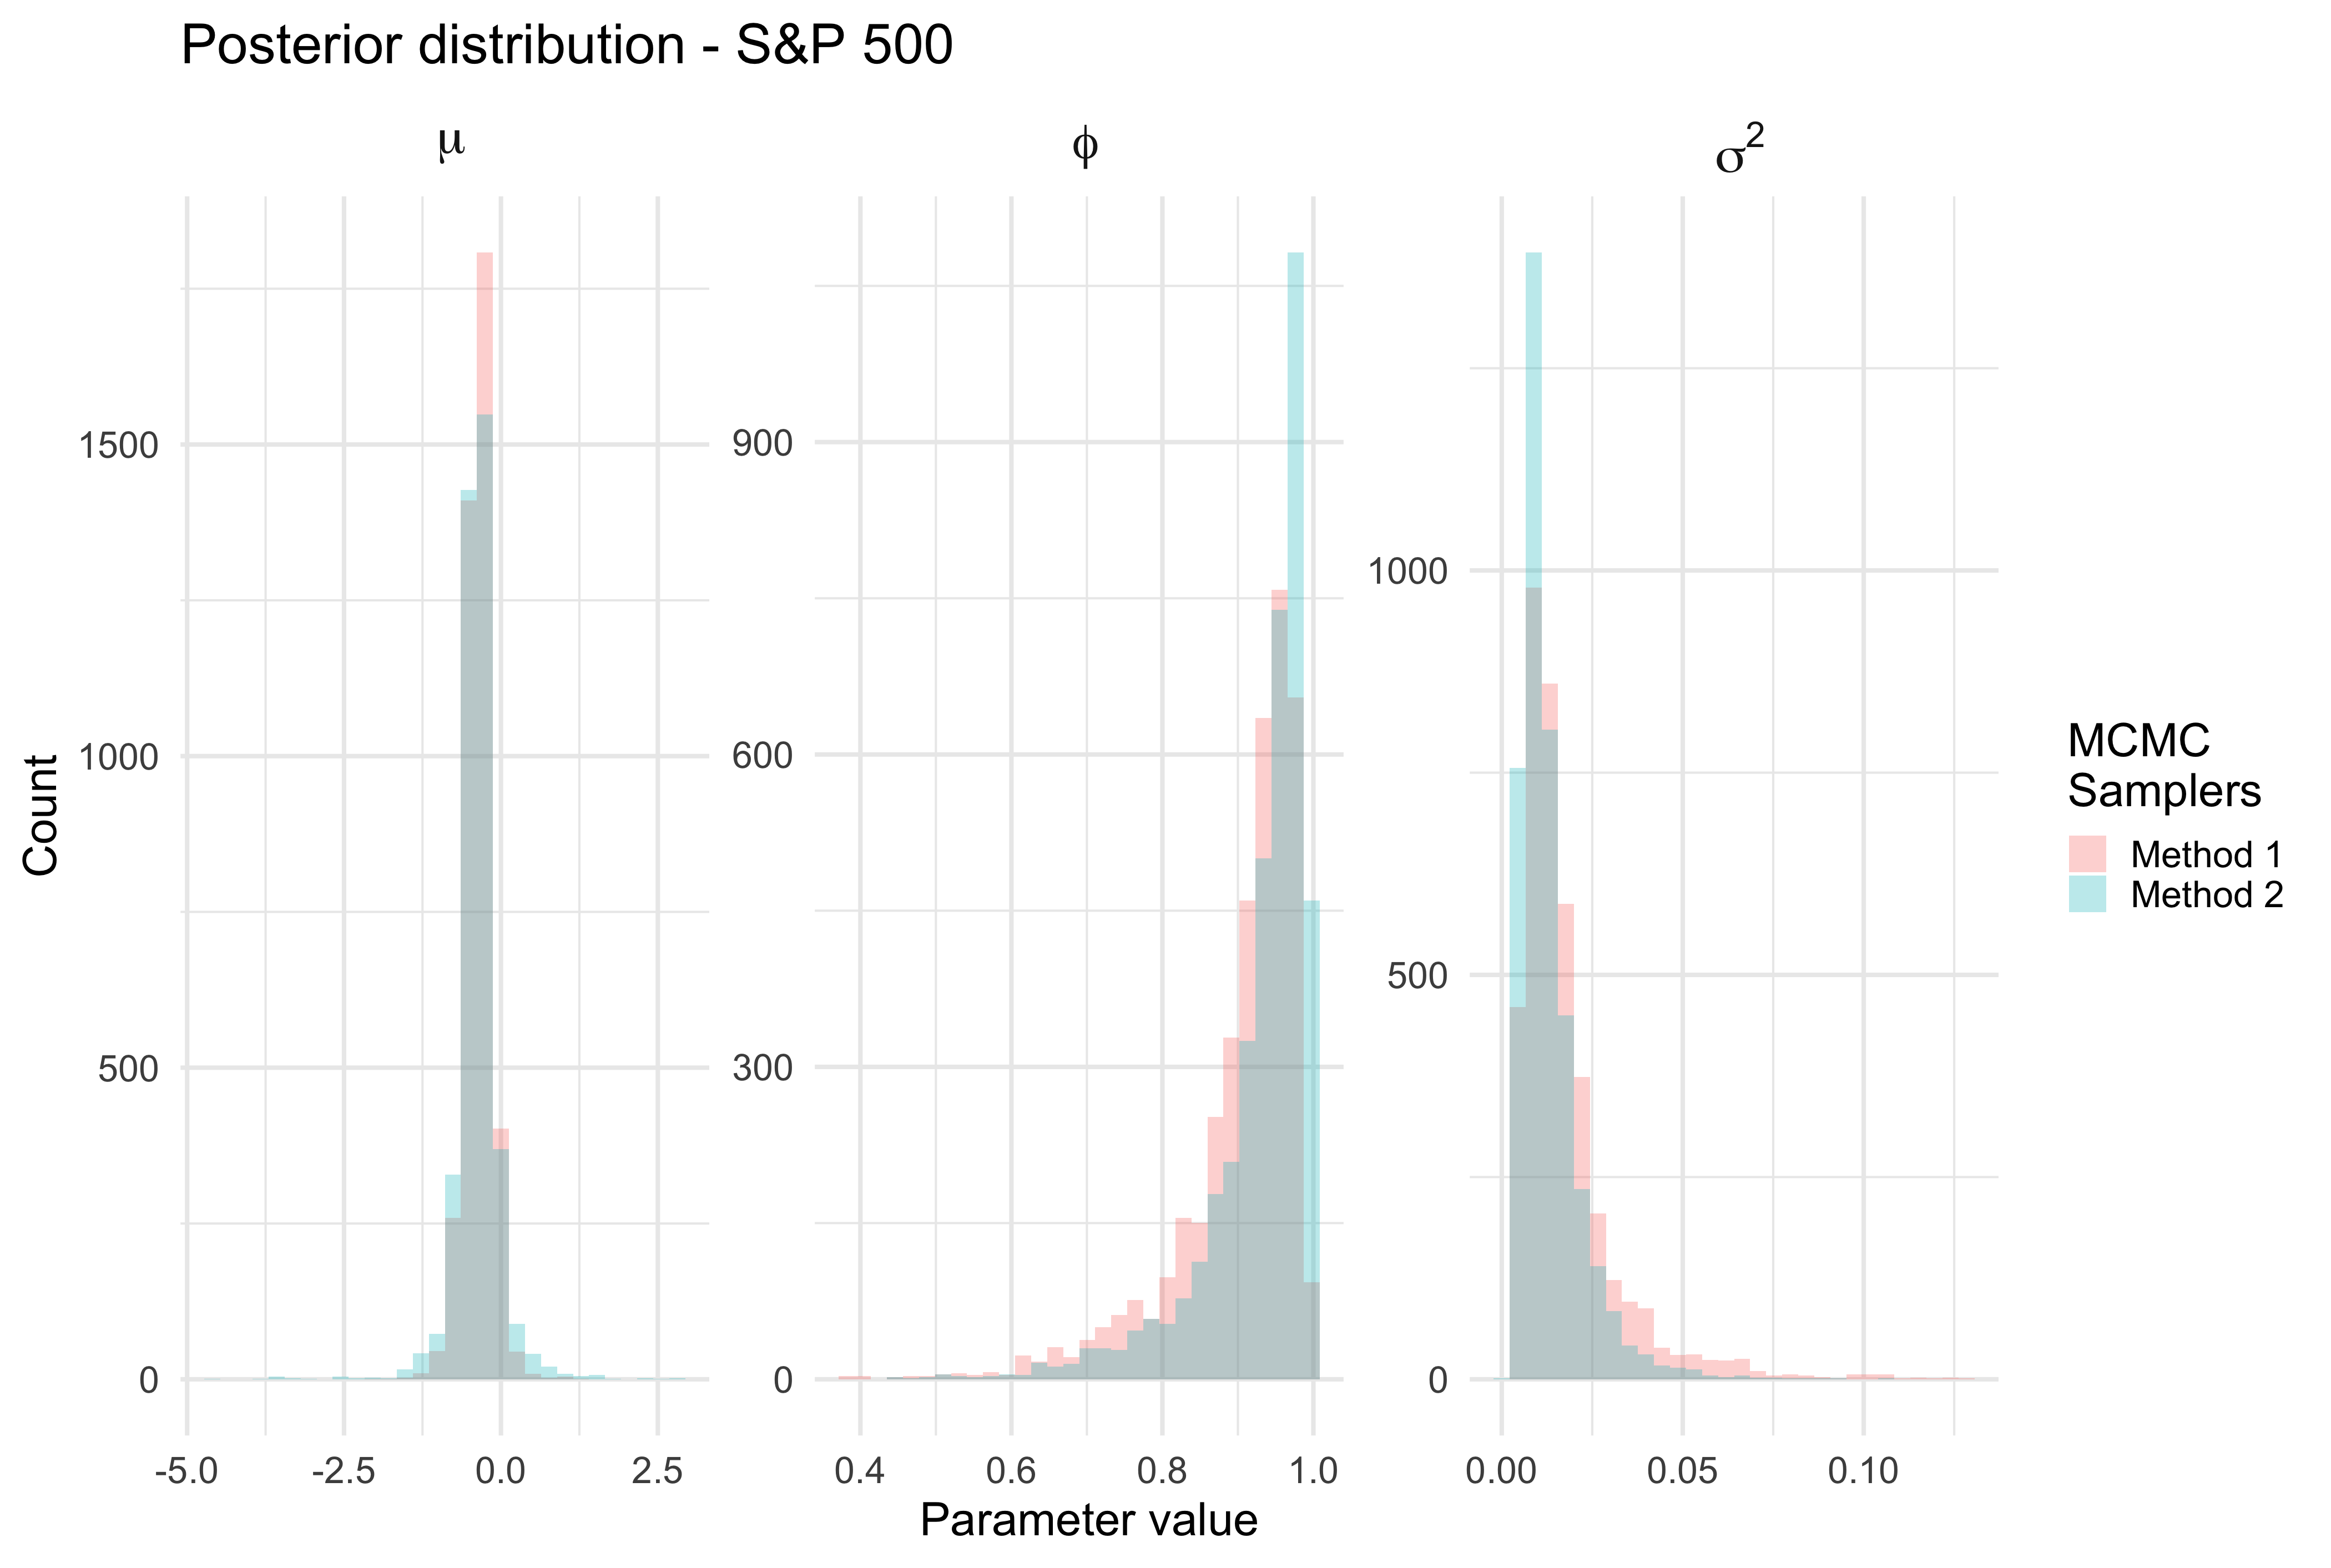
\includegraphics[scale=0.1]{motivating_example/real_data_ex.png}
        \caption{Posterior samples from two MCMC algorithms using S\&P 500 data. While the shape of the distributions are similar, the modes of method 2 is much higher and the tails of method 1 are fatter for $\phi$ and $\sigma^2$. Convergence diagnostics do not tell us which estimate is "more correct" since we don't observe the true model or true data generating process.}
    \end{figure}

    These estimates show the marginal posteriors of each parameter sharing similar shapes. $\phi$  has a fatter left tail for and $\sigma^2$ has heavier right tails for sampling method 1. Furthermore, sampling method 2 has higher peaks at their mode relative to method 1 with a tighter spread. Based on this information alone, there is no certainty in whether method 1 or method 2 is has a more correct estimate conditional on data and model. There are other methods for model or algorithmic selection in this context (for example, out of sample predictive performance), but for parameter estimation it is unclear which one should be selected. 

\subsection{Diagnostic limitations on a single simulation}
    Diagnosing computational problems on real data is difficult due to confounding factors. A strategy around this is to evaluate a model and algorithm on simulated data. One approach is to simulate data from the proposed model using known parameters. Then, fit the model on the simulated data and see if the model can recover the true parameters. This gives us the benefit of defining the true parameters of the data generating process to be estimated. If the model and algorithm cannot adequately capture the true parameter, then we cannot be confident that it will provide reliable estimates on real data.

    Furthermore, as discussed in \citet{gelman2020bayesian}, fitting models on simulated data is the only way we can check inference on latent variables. This is critical in Stochastic Volatility since the underlying framework is a state space model with latent log volatility parameters. Latent variables are unobserved in real data and are only estimated in the context of the model. Simulation gives control over the data generating process which reveals what the model can infer about the latent variables. 

    Simulations enable us to check whether our models and algorithms can estimate the true data generating process, however, there are limitations to what can be learned from a single simulation. There is always a small probability that the true parameter is in the tails of any estimated posterior distribution. Or put differently, there is a 1\% chance the true parameter or any random draw exists outside a 99\% credible interval. \cite{talts2018validating} make the point that a single simulation does not provide sufficient information about the inference made by an algorithm. As discussed in their paper, a single simulation may conclude "that an incorrectly coded analysis worked as desired, while a correctly coded analysis failed". 

    Figure 2 show the posterior distributions of a single simulation where data is generated and sampled from the stochastic volatility model with known parameters.

    \begin{figure}[h]
        \centering
        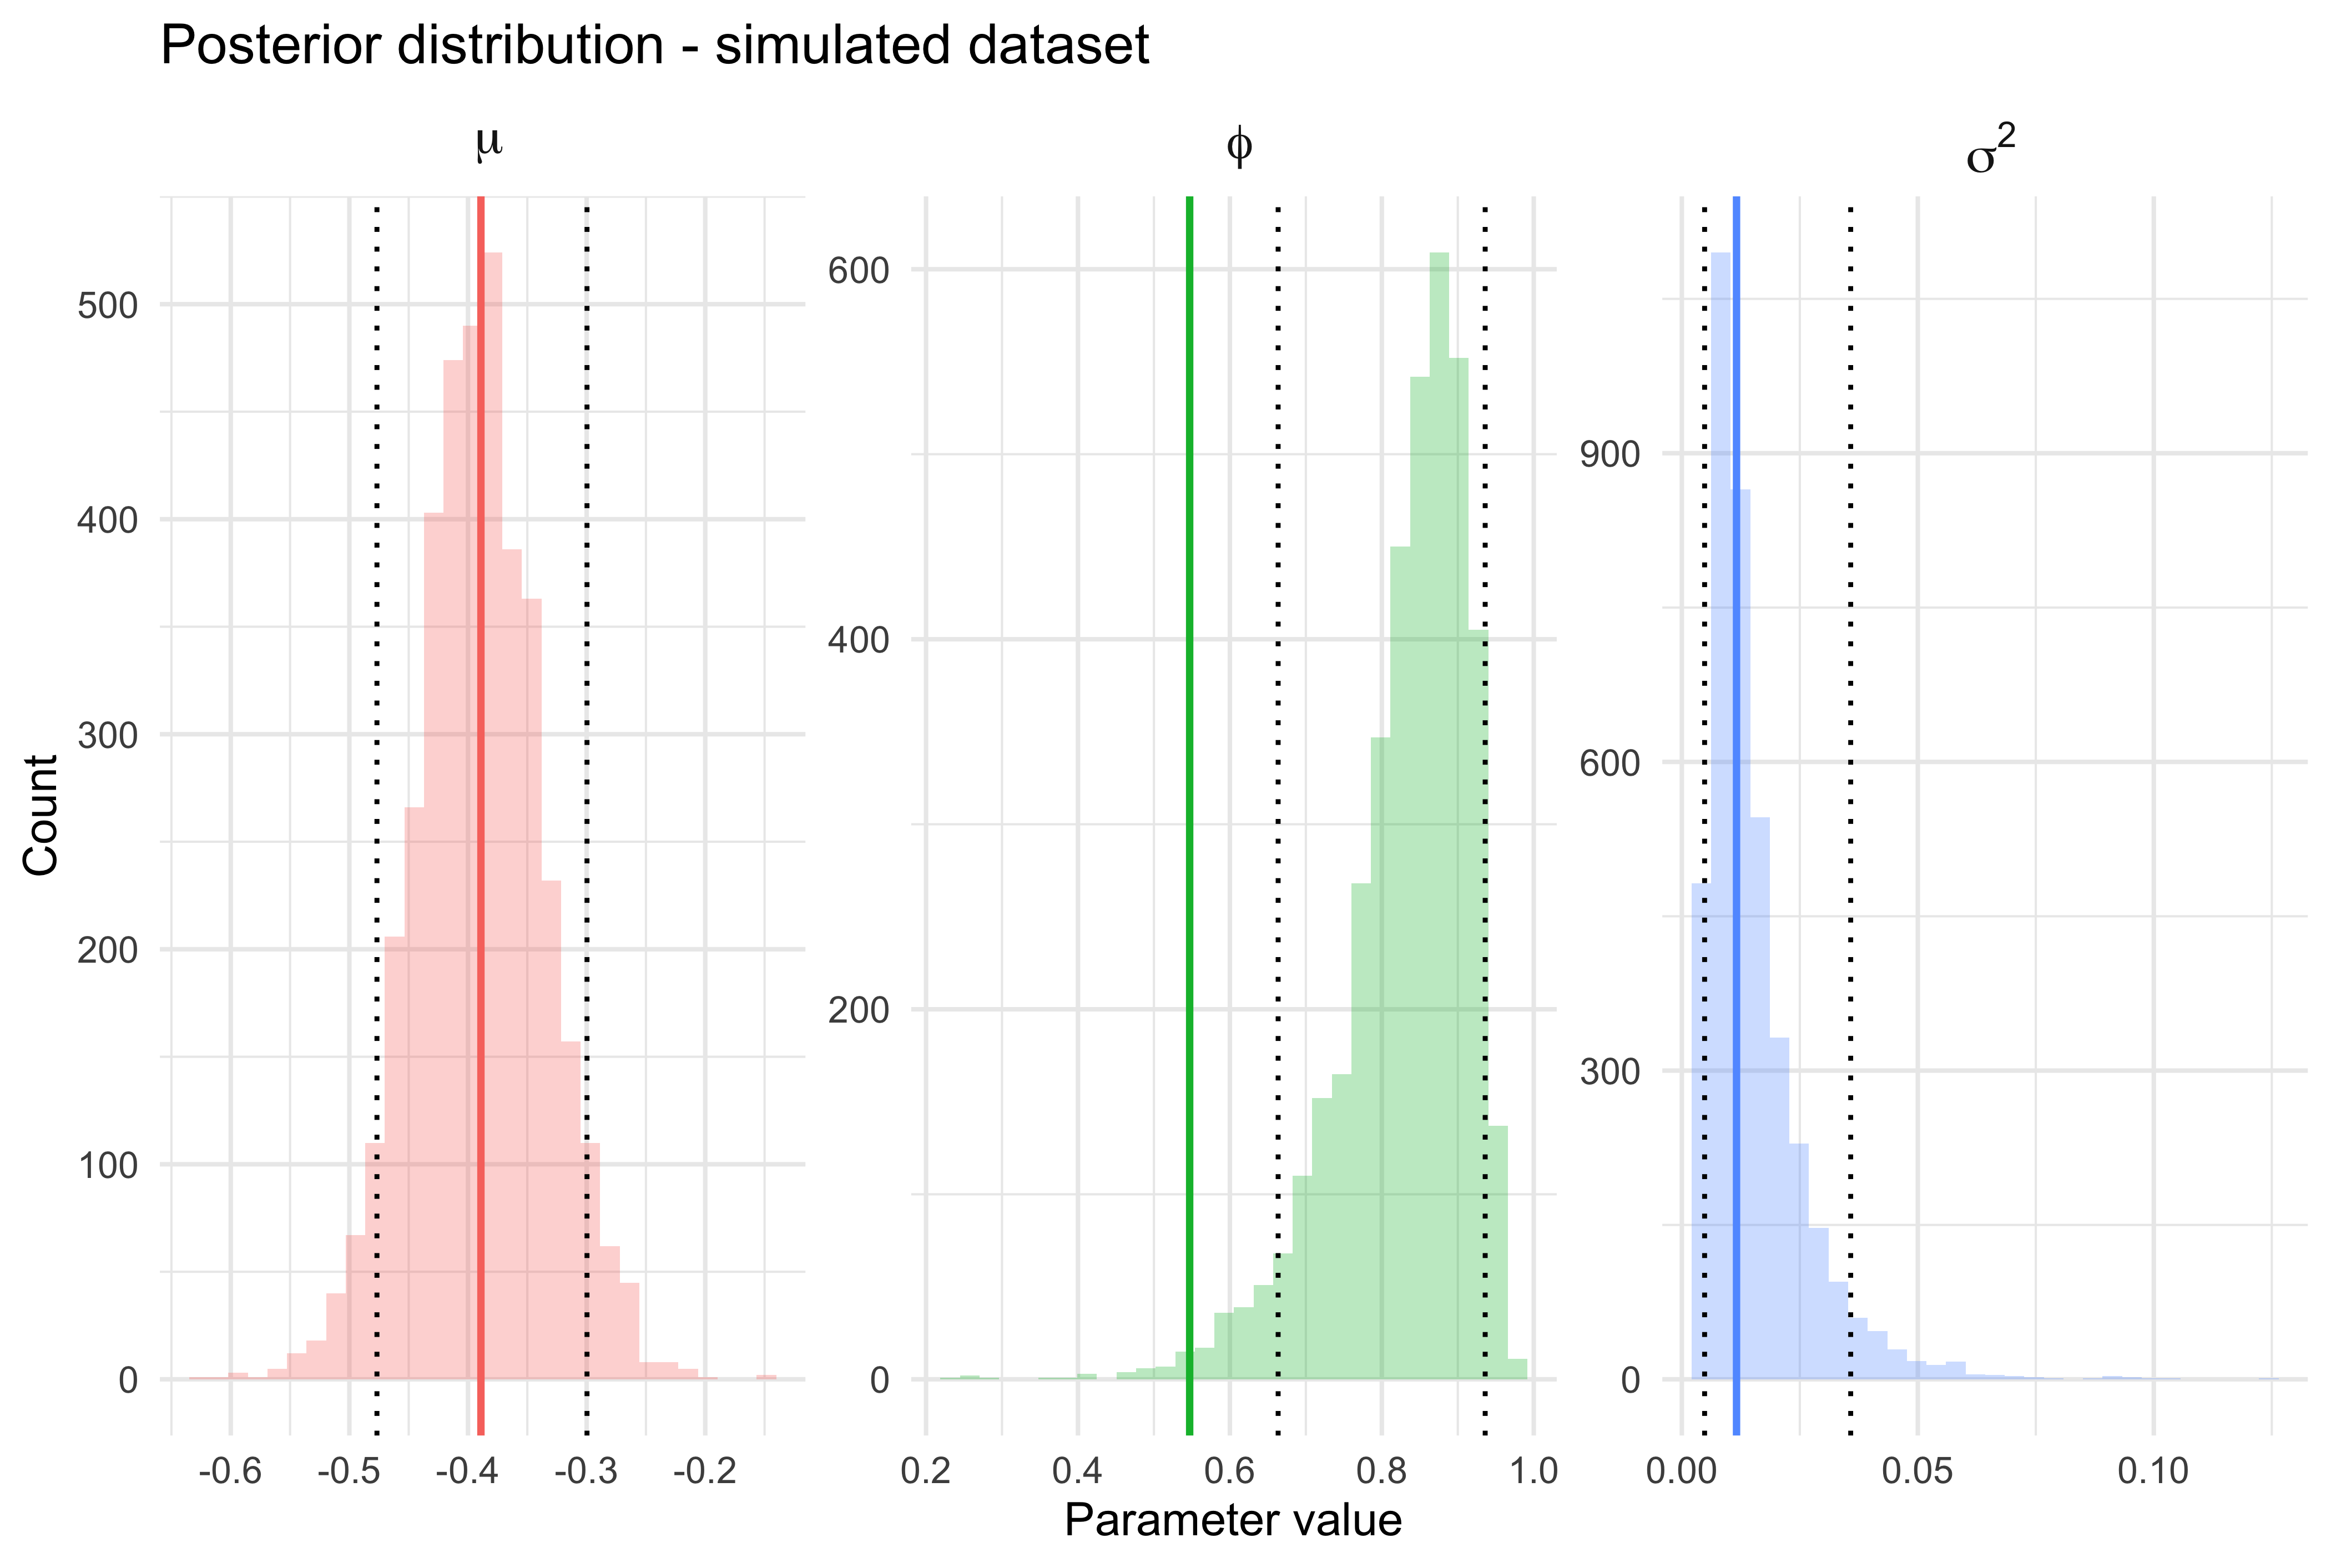
\includegraphics[scale=0.1]{motivating_example/single_sim.png}
        \caption{Posterior samples from known data genearting process. Vertical solid line represents true parameter and dotted lines are 95\% credible intervals around the mean. The parameter $\phi$ falls outside the credible interval whereas $\mu$ and $\sigma^2$ stay inside. In any one simulation conditional on the correct model, there is a 5\% probability that the true parameter falls outside this interval by chance.}
    \end{figure}

    The 95\% credible intervals for $\mu$ and $\sigma^2$ cover the true parameter. The true parameter for $\phi$ however, is in the tails and outside the interval. Such an analysis may incorrectly conclude that the model fails to adequatly estimate the $\phi$ parameter. However, it may be the case that the posterior distribution is correctly calculated using this algorithm and the results may be due to the features of this specific simulated dataset.

\subsection{Research Goal}
    The objective of this research is to design a simulation study to evaluate the calibration of algorithms used to sample Stochastic Volatility models. Indeed, there are limitations to evaluating MCMC algorithms based on fits to real data and single simulations. To check the calibration of an algorithm, simulations over multiple "true parameters" are required. This methodology is discussed in the next section. 

    Additionally, two sampling strategies will be assessed using the proposed simulation design as well as the performance of the samplers under different parameterisations of the stochastic volatility model. Not only will the calibration of any one algorithm be assessed, but also compared across sampling strategies to determine which MCMC approach is most suitable for estimating this model. 

\section{Methodology}

    \subsection{Simulation Design}
        Simulation Based Calibration (SBC) checks the calibration of posterior estimates generated by MCMC algorithms. SBC is conducted by comparing the distribution of rank statistics to the discrete uniform distribution which arises when an algorithm is correctly calibrated. The procedure starts by taking draws from the prior distribution and creating datasets implied by each draw. Rank statistics are then calculated on the posterior samples conditional on the simulated data. 

        To illustrate this procedure, let $\theta$ be a parameter and $y$ represent the dataset. Start with a single draw from the prior distribution:
        
        $$
        \begin{aligned}
        \theta^{sim} \sim \pi(\theta)
        \end{aligned}
        $$

        Generate a dataset given by the prior draw.

        $$
        \begin{aligned}
        y^{sim} \sim \pi (y|\theta^{sim})
        \end{aligned}
        $$

        Then take draws from the posterior distribution generated by a MCMC algorithm or estimation strategy (Hamiltonian Monte Carlo or KSC) conditional on this dataset.

        $$
        \begin{aligned}
        \{\theta_1,\dots , \theta_{L}\} \sim \pi (\theta | y^{sim})
        \end{aligned}
        $$

        A key result is that the posterior sample $\{\theta_1,\dots , \theta_{L}\}$ will share the same distribution as the prior samples $\theta^{sim}$. This is implied by the following expression:

        $$
        \begin{aligned}
        \pi(\theta) &= \int \pi(\theta|y^{sim}) \pi(y^{sim}|\theta^{sim}) \pi(\theta^{sim})dy^{sim} d\theta^{sim} \\
        &= \int \pi(\theta|y^{sim}) \pi(y^{sim},\theta^{sim}) dy^{sim} d\theta^{sim}
        \end{aligned}
        $$

        That is, the posterior averaged over the joint distribution follows the same distribution as the prior. The procedure of generating posterior samples implicitly performs this integral since the expression on the right of the integral is proportional to the prior density. Therefore, any deviation of the posterior samples from the prior distribution suggests that the sampling methodology is not producing the correct posteriors.

        If the posterior samples follows the prior distribution, the rank statistic for a given parameter follows a discrete uniform distribution\footnote{Proof of this result in \citet{talts2018validating}.}. The rank statistic is defined as:

        $$
        \begin{aligned}
        r = rank(\{\theta_1,\dots , \theta_{L}\}, \theta^{sim}) = \sum_{l=1}^{L}1[\theta_{l} < \theta^{sim}]
        \end{aligned}
        $$

        This completes one iteration of SBC. To complete the algorithm, multiple iterations are run and the rank statistics are calculated for each parameter. The resulting rank statistics are compared to the discrete uniform distribution to determine if any problematic features exist.

        If the computation is well calibrated and the rank statistics follow a discrete uniform distribution, then the posterior credible intervals have sufficient coverage. That is, one way to describe calibration is: for any percentage interval selected over the posterior samples (for example 90\%) then there is a 90\% chance that $\theta^{sim}$ falls within this interval. Another way of saying this is a Bayesian analysis is well calibrated if a 90\% credible interval contains the true parameter in 90\% of the SBC iterations. 

    \subsection{Evaluation Metrics}
        The key metrics and diagnostics to compare the performance of these methods are rank statistics, and chi-squared test statistics to measure calibration and the effective sample size (ESS) to measure effciency.

        \subsubsection{Rank statistics}
            As discussed in the SBC section, rank statistics are used to evaluate the calibration of the MCMC algorithm. If a posterior is well calibrated then it is expected that the distribution of rank statistics is uniform.

            The shape of the rank statistic distribution gives insight into how a MCMC may be miscalibrated. Specifically, it gives information about the type of bias in the posterior estimates for a given parameter. Figures \ref{fig:underestimation} and \ref{fig:underdispersed} are recreated from \citet{talts2018validating} for conveience which gives some examples of the posterior estimates which result in bias of the rank statistics.

            Figure \ref{fig:underestimation} shows a distribution of rank statistics with a large right peak. This is consistent with posterior samples underestimating the true parameter, where the estimated posterior distrubtion is biased to the left of the prior. The sum of indicator random variables is large since the majority of posterior draws are smaller than the true value. This results in a large rank statistic and a bias on the right side of the histogram. The coverse is true if the peak of the histogram is on the left hand side (i.e the posterior is biased towards the right hand side of the prior). 

            Figure \ref{fig:underdispersed} has large peaks on both ends of the histogram. The sampler is disproportionately over and under estimating the true parameter. \citet{talts2018validating} describe this bias as underdispersion of the posterior relative to the prior distribuion. The estimated posterior is too narrow relative to the spread of the prior resulting in bias on both ends of the rank statistics distribution. 

            % \begin{figure}[H]
            %     \centering
            %     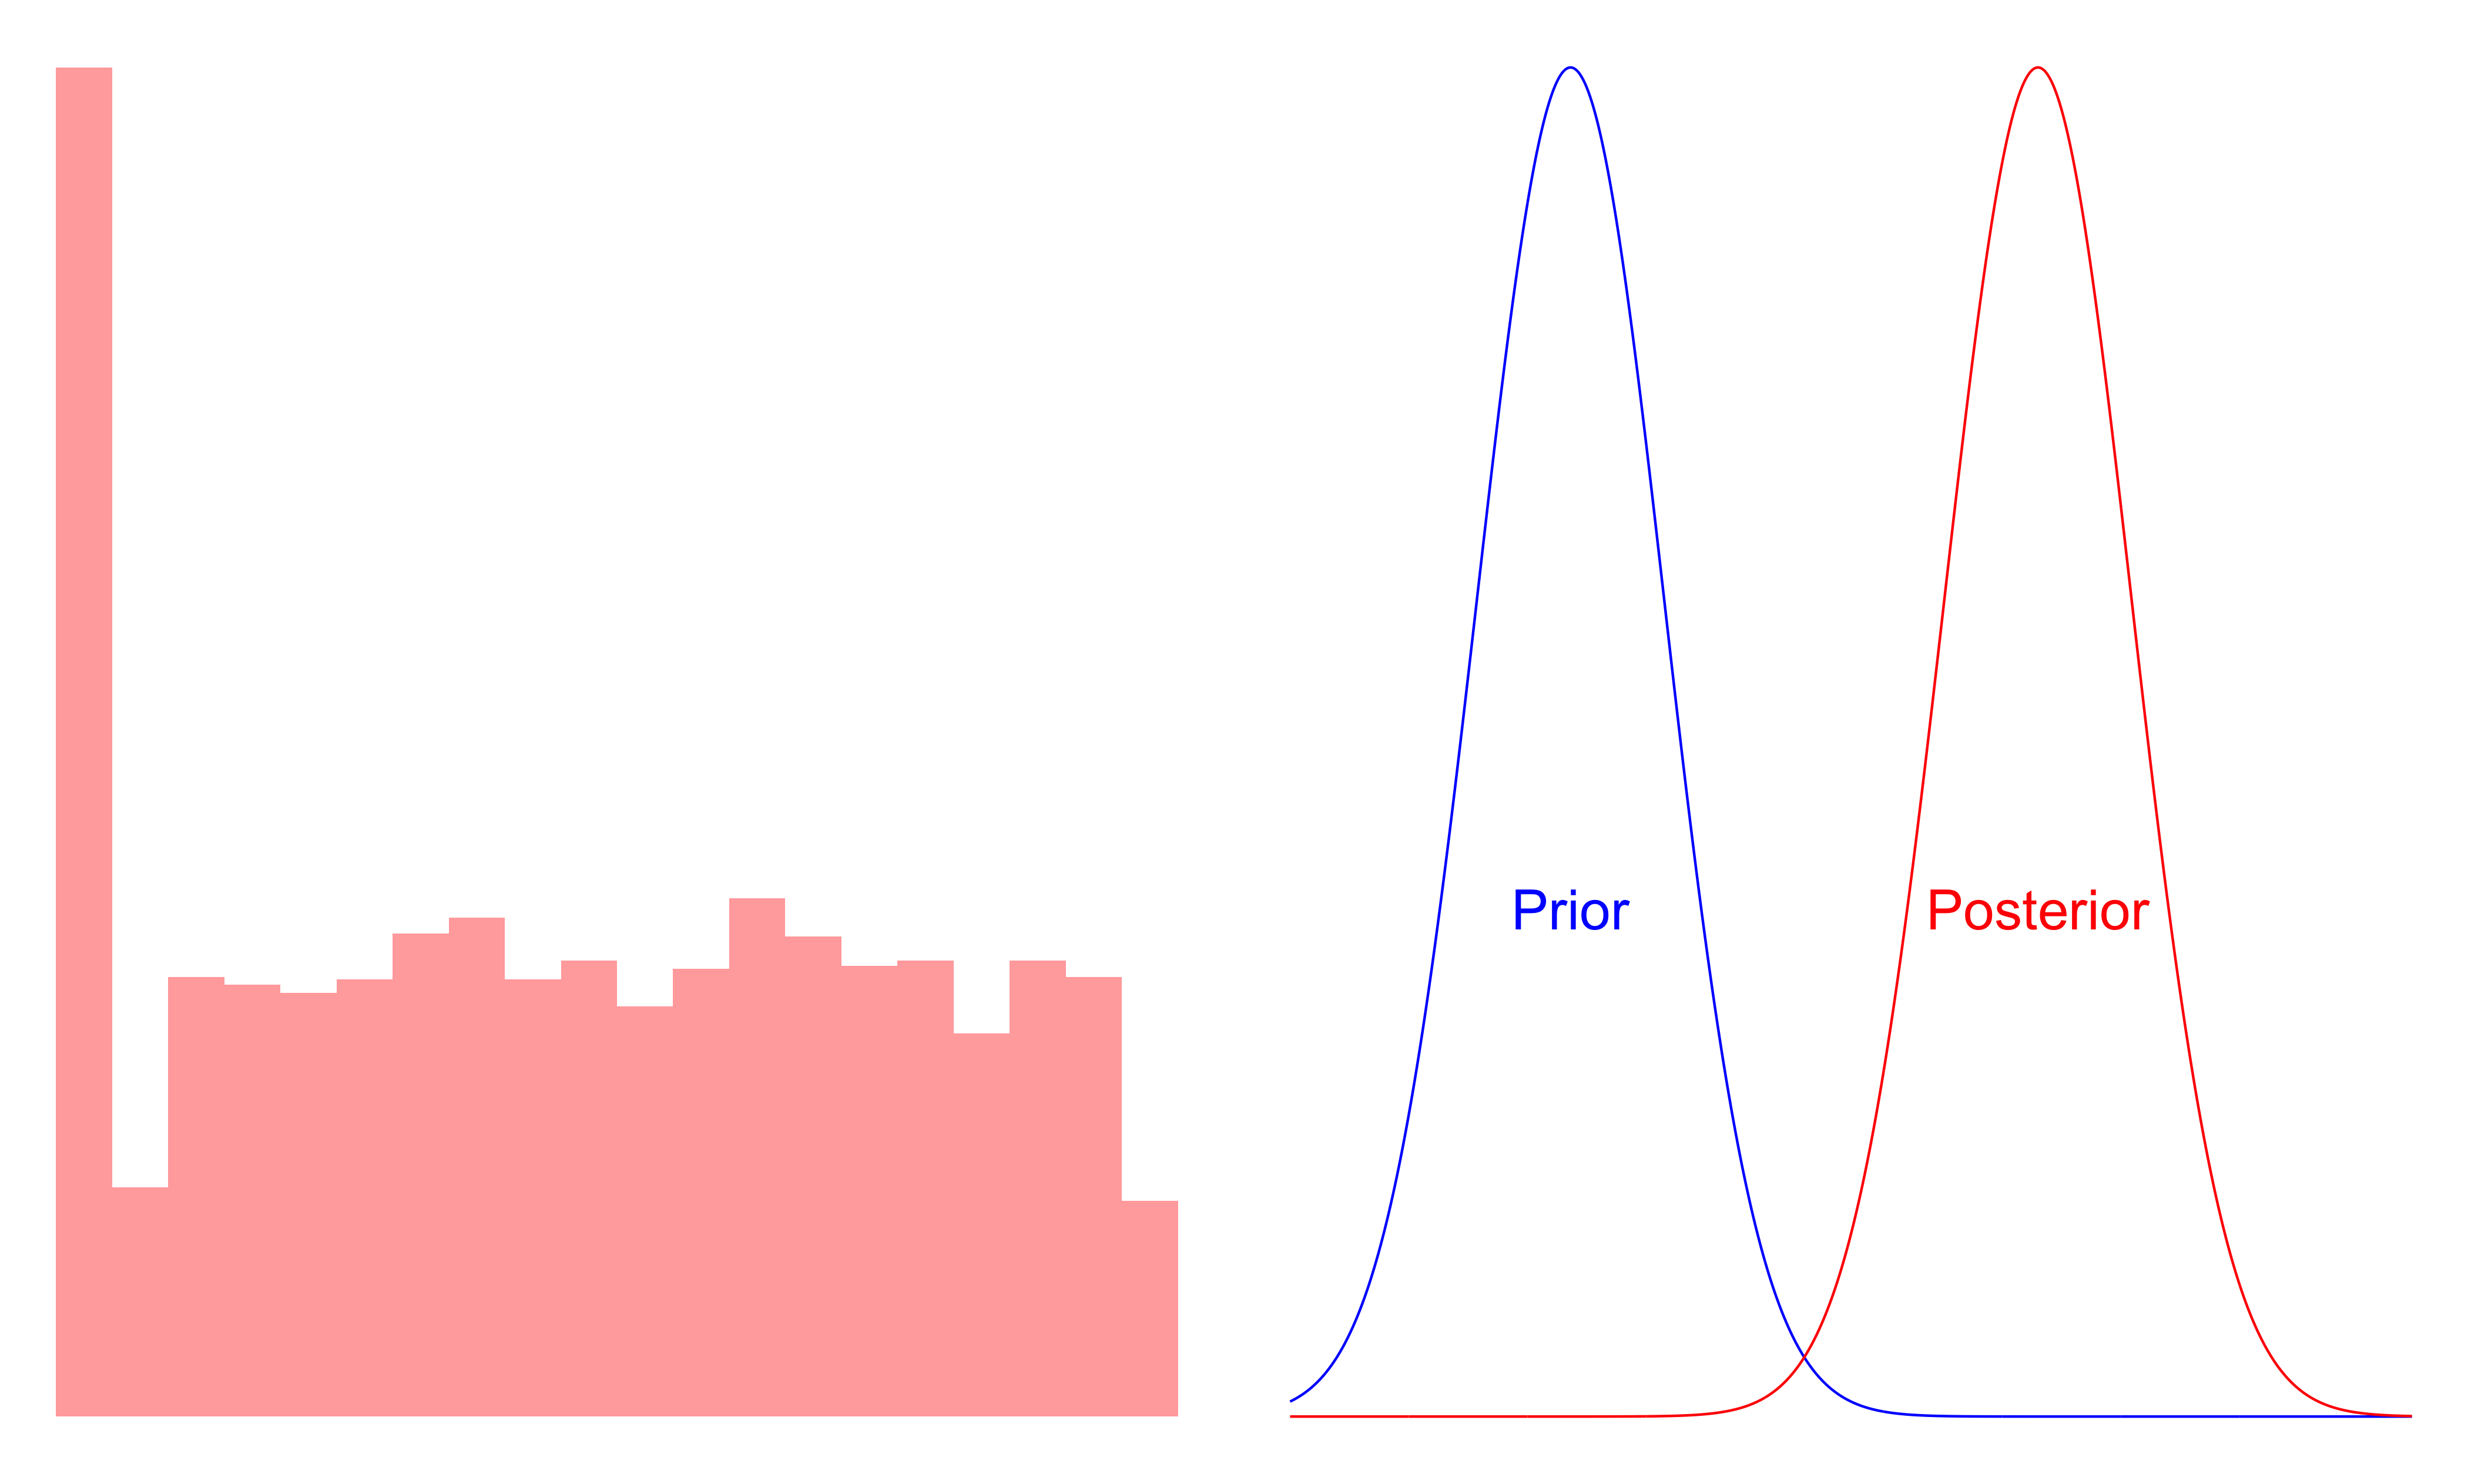
\includegraphics[scale=0.07]{methodology/lhs.png}
            %     \caption{Left: Non uniform rank statistics with peak on the left side. Right: Posterior distribution vertical line representing true parameter. Bias in rank statistics distribution comes from disproportionate number of SBC iterations overestimating the true parameter.}
            %     \label{fig:overestimate}
            % \end{figure}
        
            \begin{figure}[H]
                \centering
                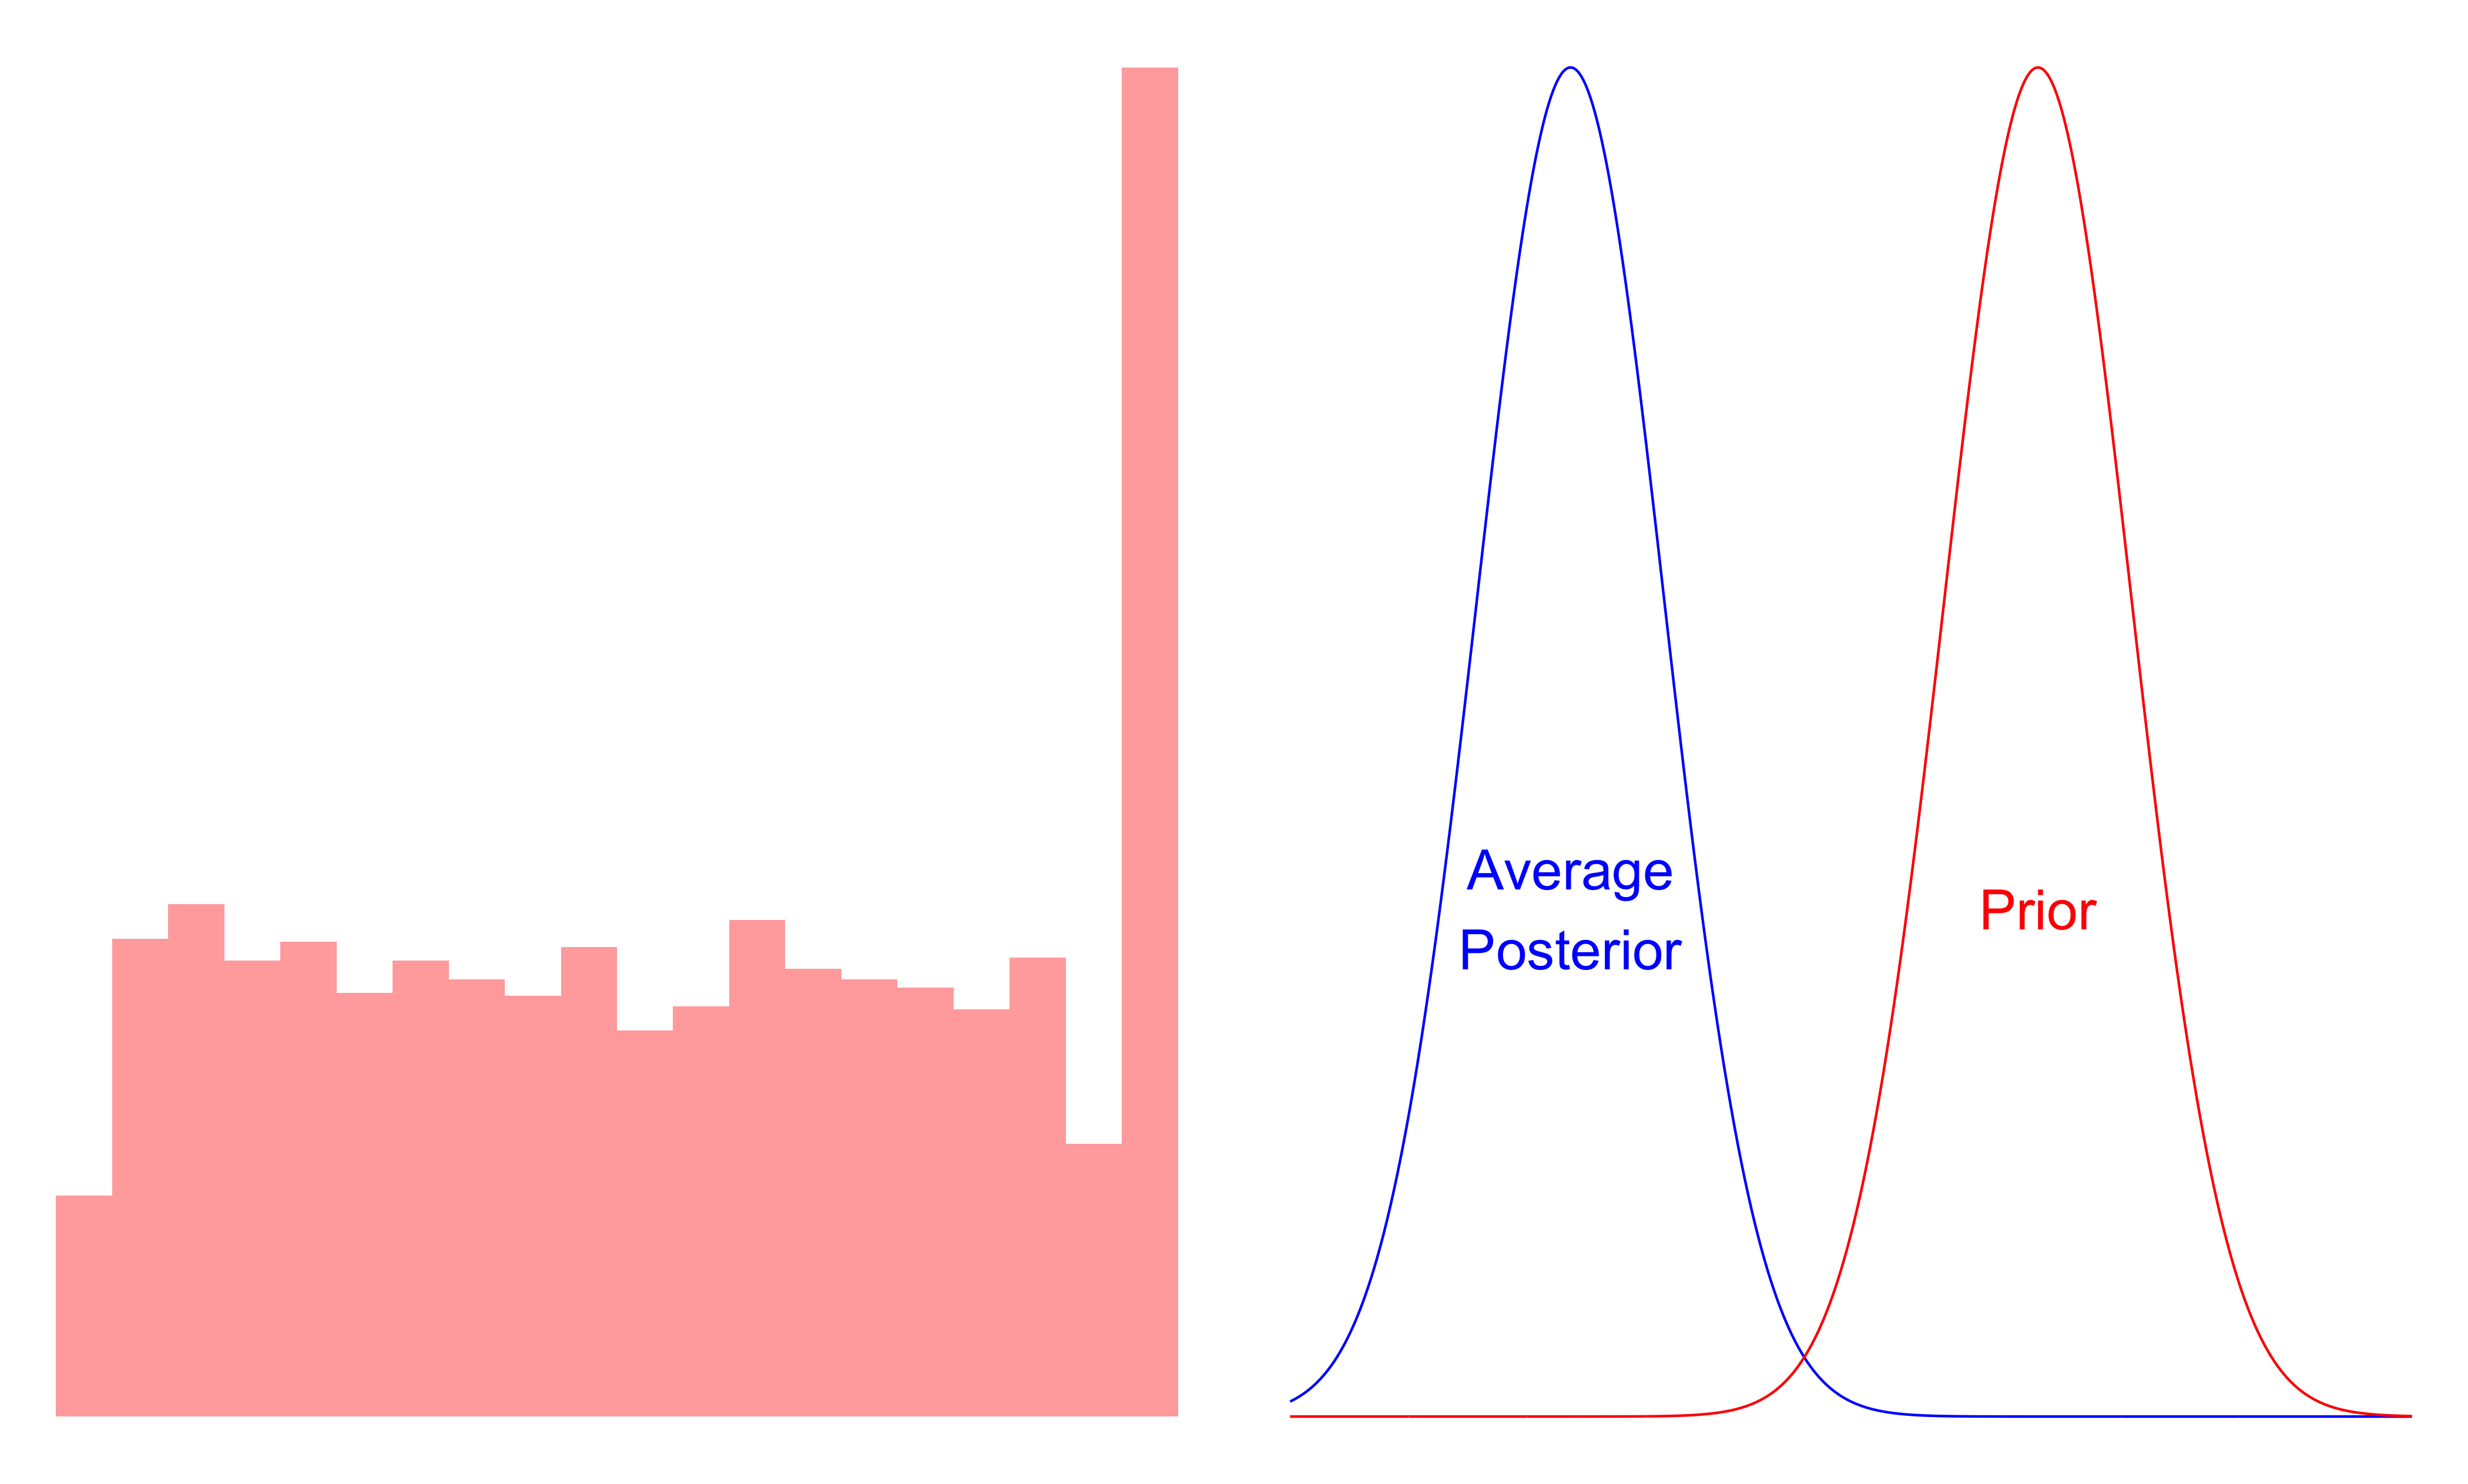
\includegraphics[scale=0.07]{methodology/rhs.png}
                \caption{Left: Non uniform rank statistics with peak on the right side. Right: Posterior distribution vertical line representing true parameter. Bias in rank statistics distribution comes from disproportionate number of SBC iterations underestimating the true parameter.}
                \label{fig:underestimation}
            \end{figure}        

            \begin{figure}[H]
                \centering
                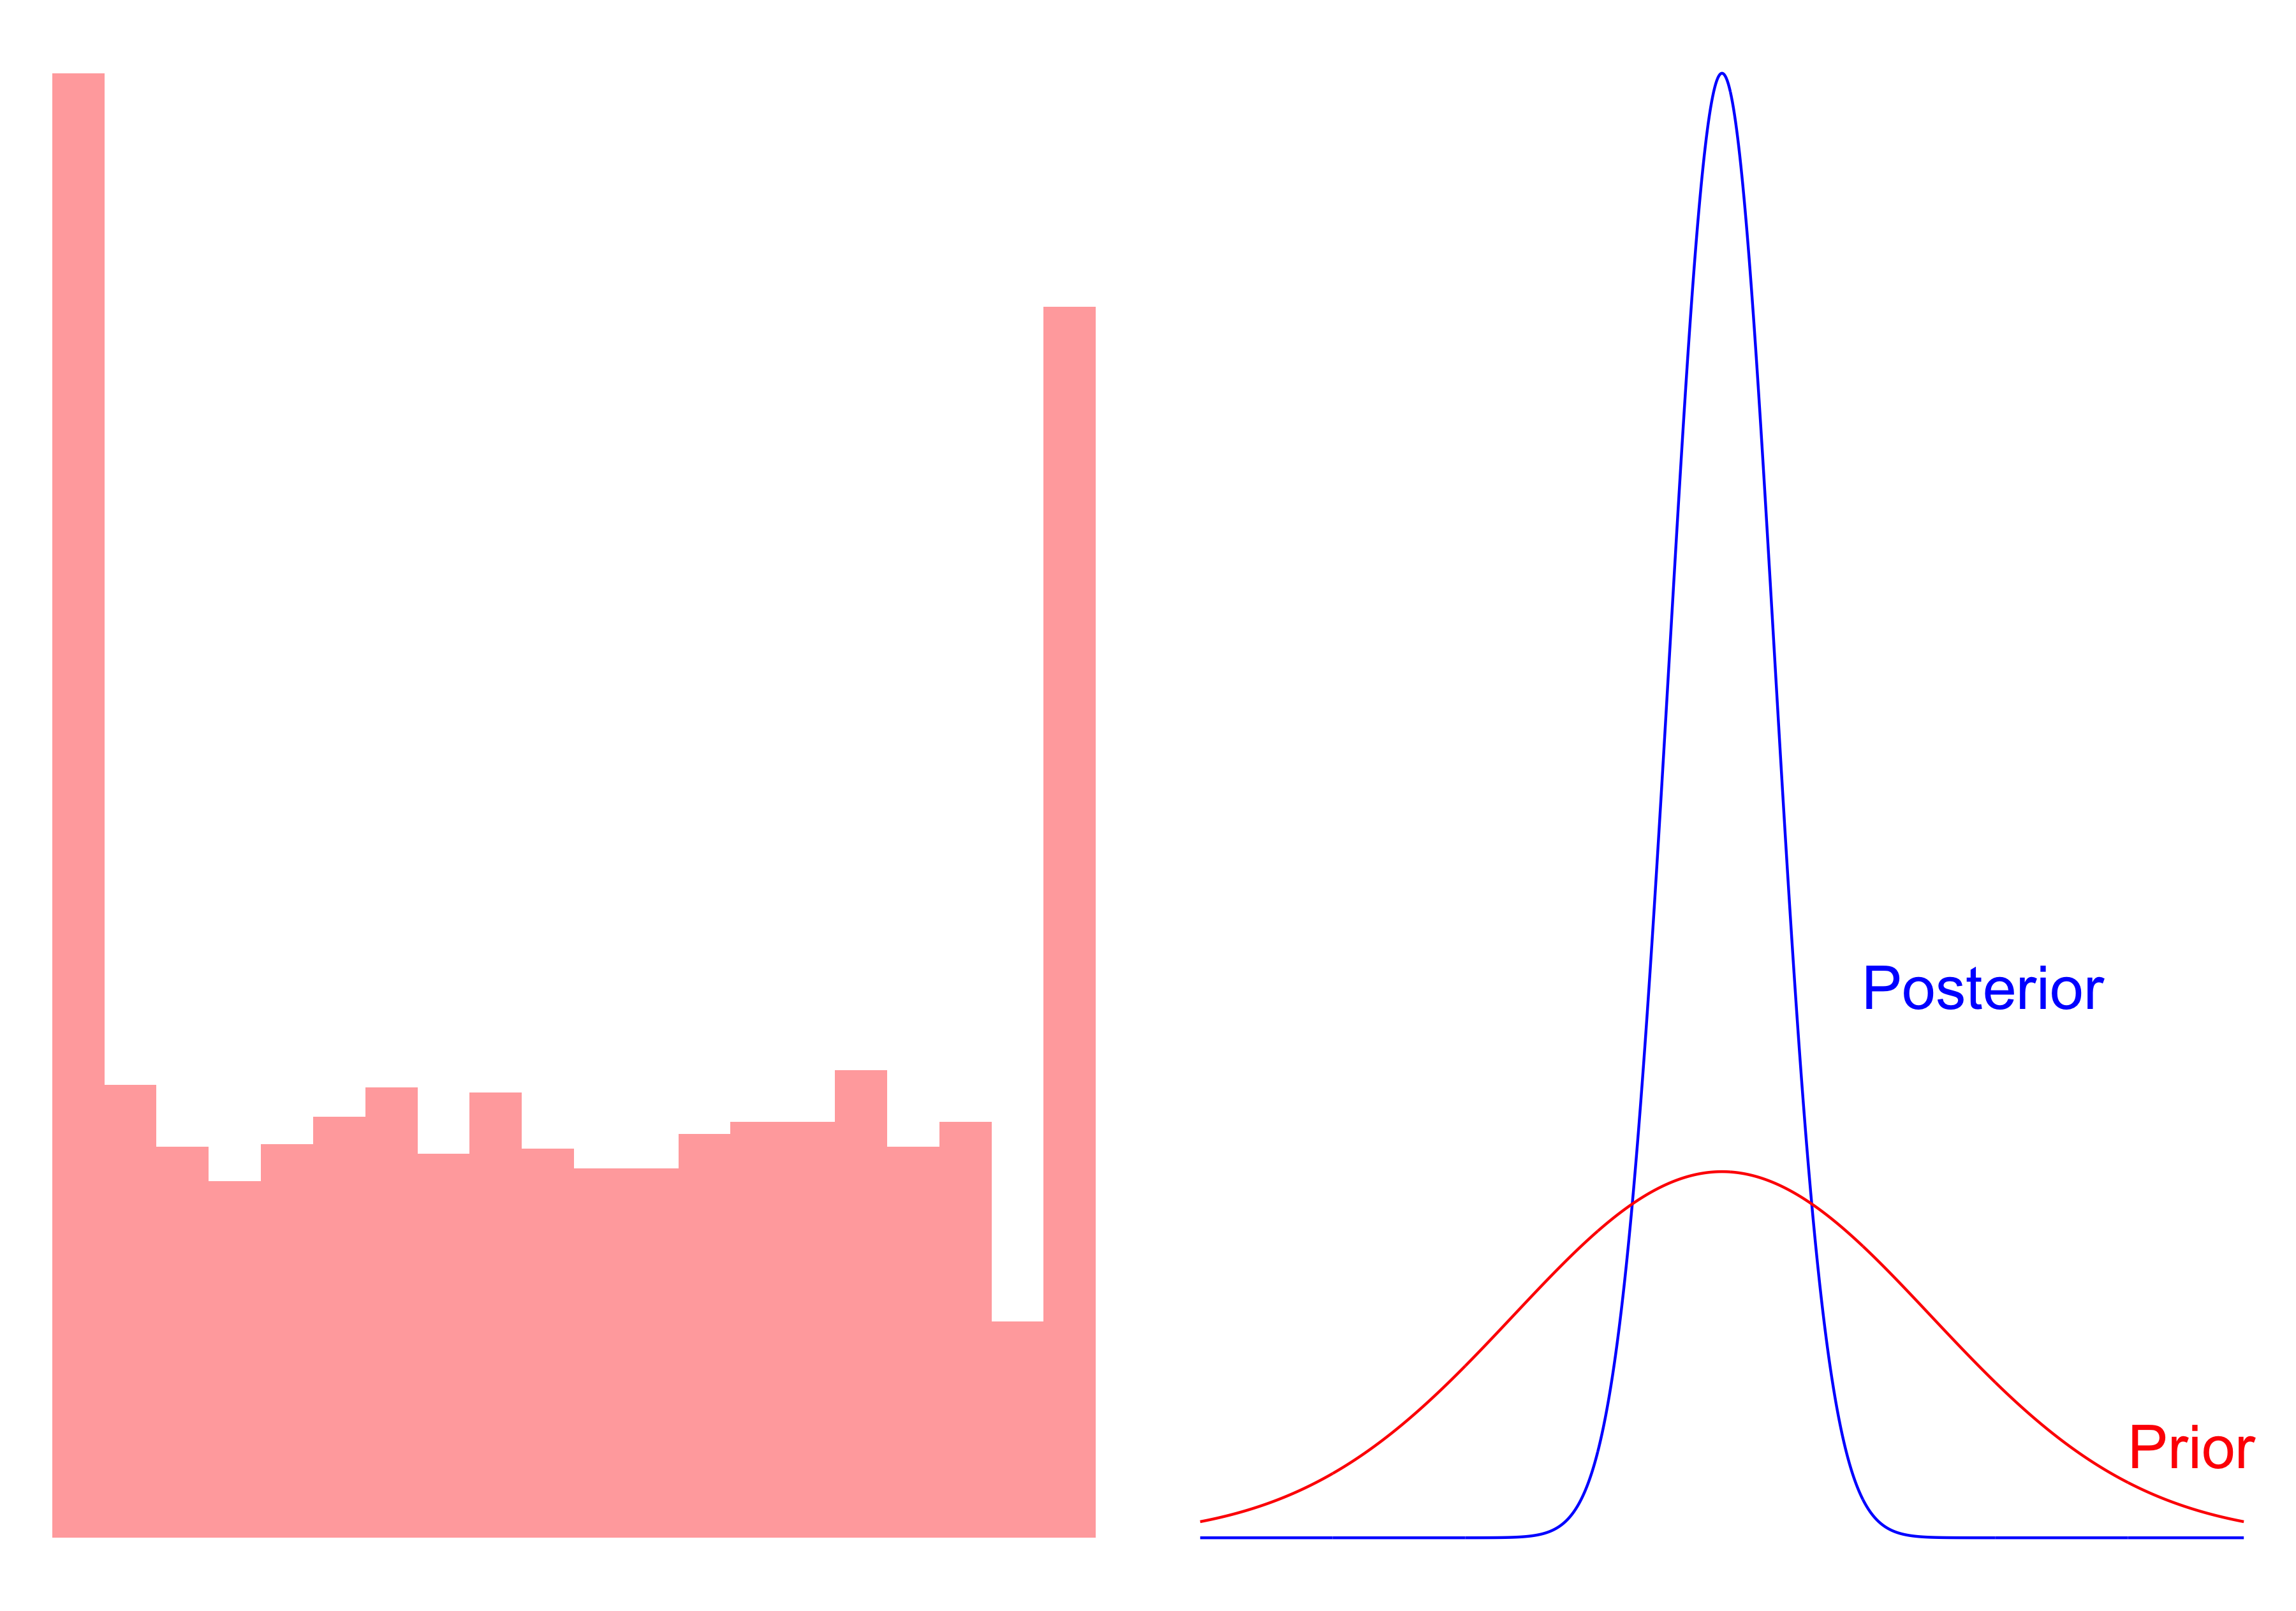
\includegraphics[scale=0.07]{methodology/underdispersed.png}
                \caption{Left: Non uniform rank statistics with peaks on both ends. Right: Overlayed posterior and prior distributions for the same arbitrary parameter. Bias in ranks comes from underdispersed posterior distribution relative to prior.}
                \label{fig:underdispersed}
            \end{figure}

            \subsubsection{Chi squared statistics}
            A drawback from visualising the rank statistic distributions is there are more parameters (1003 parameters) than data points in this model. An alternative to visually checking for uniformity of all the parameters is to calculate the chi squared statistics for the counts in each histogram bin. Let $b_j$ be the number of counts and $e_j$ the expected count in bin $j$. Then the chi squared statistic is given by:
            
            $$
            \begin{aligned}
            \chi^2 = \sum_{j=1}^J \frac{(b_{j} - e_{j})^2}{e_j}
            \end{aligned}
            $$
            
            A perfectly discrete uniform distribution will return a $\chi^2$ statistic of zero. That is, the number of rank statistics in each bin is equal to the expected number conditional on the number of bins and observations. Instead of performing multiple hypothesis tests for each parameter, the distribution of $\chi^2$ statistics is compared across all parameters and simulations. This will give a high level summary of calibration and overall performance of the algorithms.

            \subsubsection{Effective sample size}
            ESS measures the efficiency of the MCMC sampler. It calculates the number of effectively independent draws generated by a MCMC to estimate a target parameter. A poor ESS can arise from high autocorrelation in the Markov chain which leads to highly dependent samples. An efficient MCMC algorithm takes less resources (for example, time and number of draws) to get a representative sample of the target distribution. If a MCMC algorithm possesses higher ESS for the majority of its parameters (relative to another strategy), then there is evidence that this method is a more efficient sampler.
            
            The ESS is defined as $n_{eff}$ and is a function of the number of chains $M$, the number of samples per chain $N$ and the autocorrelation at lag t $\rho_t$. $T$ is a trunction lag chosen such that the sum of any two consecutive autocorrelation lags is negative. This truncation (or some kind of downweighting) is required because a large number of lags leads to noiser autocorrelation estimates. More details about this and the calculation of the autocorrelation can be found in \citep{vehtari2021rank} and \citet{geyer1992practical}.

            $$
            \begin{aligned}
                n_{eff} = \frac{NM}{1+2 \sum_{t=1}^T \hat{\rho}_t}
            \end{aligned}
            $$

\section{MCMC Strategies}

    \subsection{Sampling method 1}
        (KSC) sample the posteriors of the stochastic volatility model using a mix of conjugate posterior distributions, Metropolis Hastings and the Kalman Filter and smoother\footnote{In this research the exact software to apply the simulation smoother is unavailable, so a more recent simulation smoother is used which is based on the software written by the same author.} \citep{dejong1995}.

        The standard Kalman Filter and smoother is used to compute the posterior distribution over the latent states. This requires the state and measurement equations to be linear and conditionally Gaussian. Since the relationship between $y_t$ and $h_t$ in the measurement equation is not linear, a transformation is applied by squaring and taking the log of $y_t$.

        $$
        \begin{aligned}
        y_t^{*} &= log(y_t^2) \\ 
        &= log((\epsilon_t exp(h_t/2))^2) \\
        &=  log(exp(h_t)) + log(\epsilon_t^2) \\
        &= h_t + log(\epsilon_t^2)  \\
        &= h_t + z_t \\
        \end{aligned}
        $$

        Where $z_t = log(\epsilon_t^2)$ follows a log chi-squared distribution with mean -1.2704 and variance 4.93. The relationship between $y_t$ and $h_t$ is now linear; however, the error is not Gaussian. Since it is not simple to sample from this parameterisation of the model, KSC use a mixture of Gaussians to **approximate** the first 4 moments of the log chi squared distribution. This is defined by:

        $$
        \begin{aligned}
        f(z_t) = \sum_{i=1}^{K} q_if_N(z_i|m_i-1.2704, \nu_i^2)
        \end{aligned}
        $$

        Where K is the mixture of normal densities $f_N$, component probabilities $q_i$, mean $m_i-1.2704$ and variance $\nu_i^2$. These parameters were selected using moment matching where they found 7 normal densities with varying mean and variance parameters best approximated the log chi squared moments. These parameters and weights can be found in Appendix A.

        The model can be sampled via the Kalman Filter and simulation smoother since the model is now linear and conditionally gaussian. The static parameters $\mu$ and $\sigma^2$ are sampled directly from their conjugate posterior distributions whereas $\phi$ is sampled via a Metropolis Hastings accept/reject procedure. The details can be around in Appendix B. 

    \subsection{Sampling method 2}
    % Need much more detail here about how it works
        Since the paper was written, new MCMC algorithms have been developed and enabled the estimation of richer and more complicated models. Specifically, Hamiltonian Monte Carlo is a MCMC algorithm which has become widely available for efficiently sampling from sophisticated models. Hamiltonian Monte Carlo, originally called Hybrid Monte Carlo, was developed in the physics literature \citep{duane1987hybrid} before being applied in the statistics literature by Radford Neal through his works in Bayesian Neural Networks \citep{neal1995bayesian} and statistical computing \citep{neal2011mcmc}. The algorithm has since become widely available through open source development projects such as Stan \citep{stan} and PyMC \citep{pymc2023}.

        The key innovation of Hamiltonian Monte Carlo is using the gradients of the target posterior distribution to generate an efficient path for the sampler to explore. Unlike Random Walk Metropolis Hastings, it takes advantage of the geometry of the posterior to determine its next proposal step. A comprehensive explanation of the sampler is beyond the scope of this research and can be found in the above references. 

        The Stan programming language's implementation of Hamiltonian Monte Carlo will be used for this study. Stan's default algorithm, the No-U-Turn Sampler \citep{hoffman2014no}, allows for direct sampling of the specified stochastic volatility model. Hamiltonian Monte Carlo allows for sampling of the generative model and can flexibly handle complicated likelihood functions. This approach will also use the same priors as specified in the Gaussian mixture approximation.

    \subsection{Model Parameterisation}

        The parameterisation of a model can affect the performance of a MCMC algorithm when sampling from models with complex posterior geometries. An example of this is Neal's funnel \citep{neal2003slice} where the Hamiltonian Monte Carlo sampler encounters performance issues in hierarchical models and produces biased samples. Efficiency improvements of MCMC algorithms for state space models under different parameterisations are also explored \citet{strickland2008parameterisation}.

        The stochastic volatility model as described in section 2.1 is follows a "centered" parameterisation. This describes the central location of the latent state parameters which are centered around the mean and lag of the log volatility $\mu +\phi(h_t - \mu)$. A model can be reparameterised such that the states are sampled on a distribution centered on 0 (i.e "non centered") which are later transformed to have the correct mean. The following re-parameterisations are explored as part of the simulation study.
        
        \subsubsection{Non centered Hamiltonian Monte Carlo}
        First sample from a standard normal distribuition and multiply by the variance of the log volatility. The state variable is sampled with mean centered on zero and variance equal to $\sigma_{\eta}^2$

        $$
        \begin{aligned}
        h_{std} \sim& \space normal(0,1) \\
        h =& h_{std} \times \sigma_{\eta} \\ 
        h \sim& normal(0, \sigma_{\eta}^2)
        \end{aligned}
        $$
        
        Then apply the appropriate rescaling to get samples from log volatility. 
        
        $$
        \begin{aligned}
        h_1 =& \space \frac{h_{std, 1}\times \sigma_{\eta}} {\sqrt{1 - \phi^2}} + \mu \\
        h_{t+1} =& \space h_{std, t+1}\times \sigma_{\eta} + \mu  + \phi(h_{t} - \mu),\space t\neq 1
        \end{aligned}
        $$
        
        This returns log volatility as desired.
        
        $$
        \begin{aligned}
        h_1 \sim& \space normal \left(\mu, \frac{\sigma_{\eta}^2}{1-\phi^2}\right) \\
        h_{t+1} \sim& \space normal(\mu +\phi(h_t - \mu) , \sigma_{\eta}^2), \space\space t\neq 1\\ 
        \end{aligned}
        $$

        \subsubsection{Non centered Gaussian Mixture}
        The non centered model for the Gaussian approximation is expressed slightly differently due to the use of the Kalman Filter. Non centered HMC samples from the joint posterior directly with state vectors centered at zero and transformed to return the correct log volatility estimates. Applying the Kalman Filter requires the state equation to be a function of the state variable with the average log volatility parameter $\mu$ entering the measurement equation.
        
        Starting with the log chi squared model:

        $$
        \begin{aligned}
        y^{\ast}_t =& h_t + z_t \\
        h_{t+1} =& \space \mu +\phi(h_t - \mu) + \sigma_{\eta} \eta_t
        \end{aligned}
        $$
        

        Let $g$ be the demeaned state variable. Rewrite the demeaned state equation $g_{t+1}$ to be non centered in location by subtracting average volatility $\mu$.

        $$
        \begin{aligned}
        g_t =& h_t - \mu \\
        g_{t+1} =& \phi g_t + \sigma_{\eta}\eta_{t}
        \end{aligned}
        $$

        Return average volatility into measurement equation and rewrite as a function of the non centered state equation:

        $$
        \begin{aligned}
        y^{\ast}_t =& g_t + \mu + z_t \\
        g_{t+1} =& \phi g_t + \sigma_{\eta}\eta_{t}
        \end{aligned}
        $$

        The mean of the log volatility is now inside the measurement equation and de-meaned from the state equation.
    
    \subsubsection{Prior Predictive check}
        It is worth noting that the centered and non-centered parameteristions are the same stochastic volatility model. Different parameteristions express the same mathematical models in ways that make it easier or harder for a given algorithm to sample. 

        To demonstrate this, a prior predictive simulation of the second state parameter is performed for both a centered and non centered model (using the paramterisation described in section 3.3.1). This is the same as the first two steps of SBC, except instead of generating a dataset, generate the parameters implied by the prior draw. Let $\boldsymbol{\theta}$ be a vector of static parameters.

        $$
        \begin{aligned}
        \boldsymbol{\theta}^{sim} \sim \pi(\boldsymbol{\theta})
        \end{aligned}
        $$

        Generate a the second state parameter implied by the joint prior.

        $$
        \begin{aligned}
        h_2^{sim} \sim \pi (h_2|h_1, \boldsymbol{\theta}^{sim})
        \end{aligned}
        $$

        Generating 1000 samples of $h_2^{sim}$ from both centered and non-centered models gives samples from the same data generating process as shown in figure 3. 


        \begin{figure}[h]
            \centering
            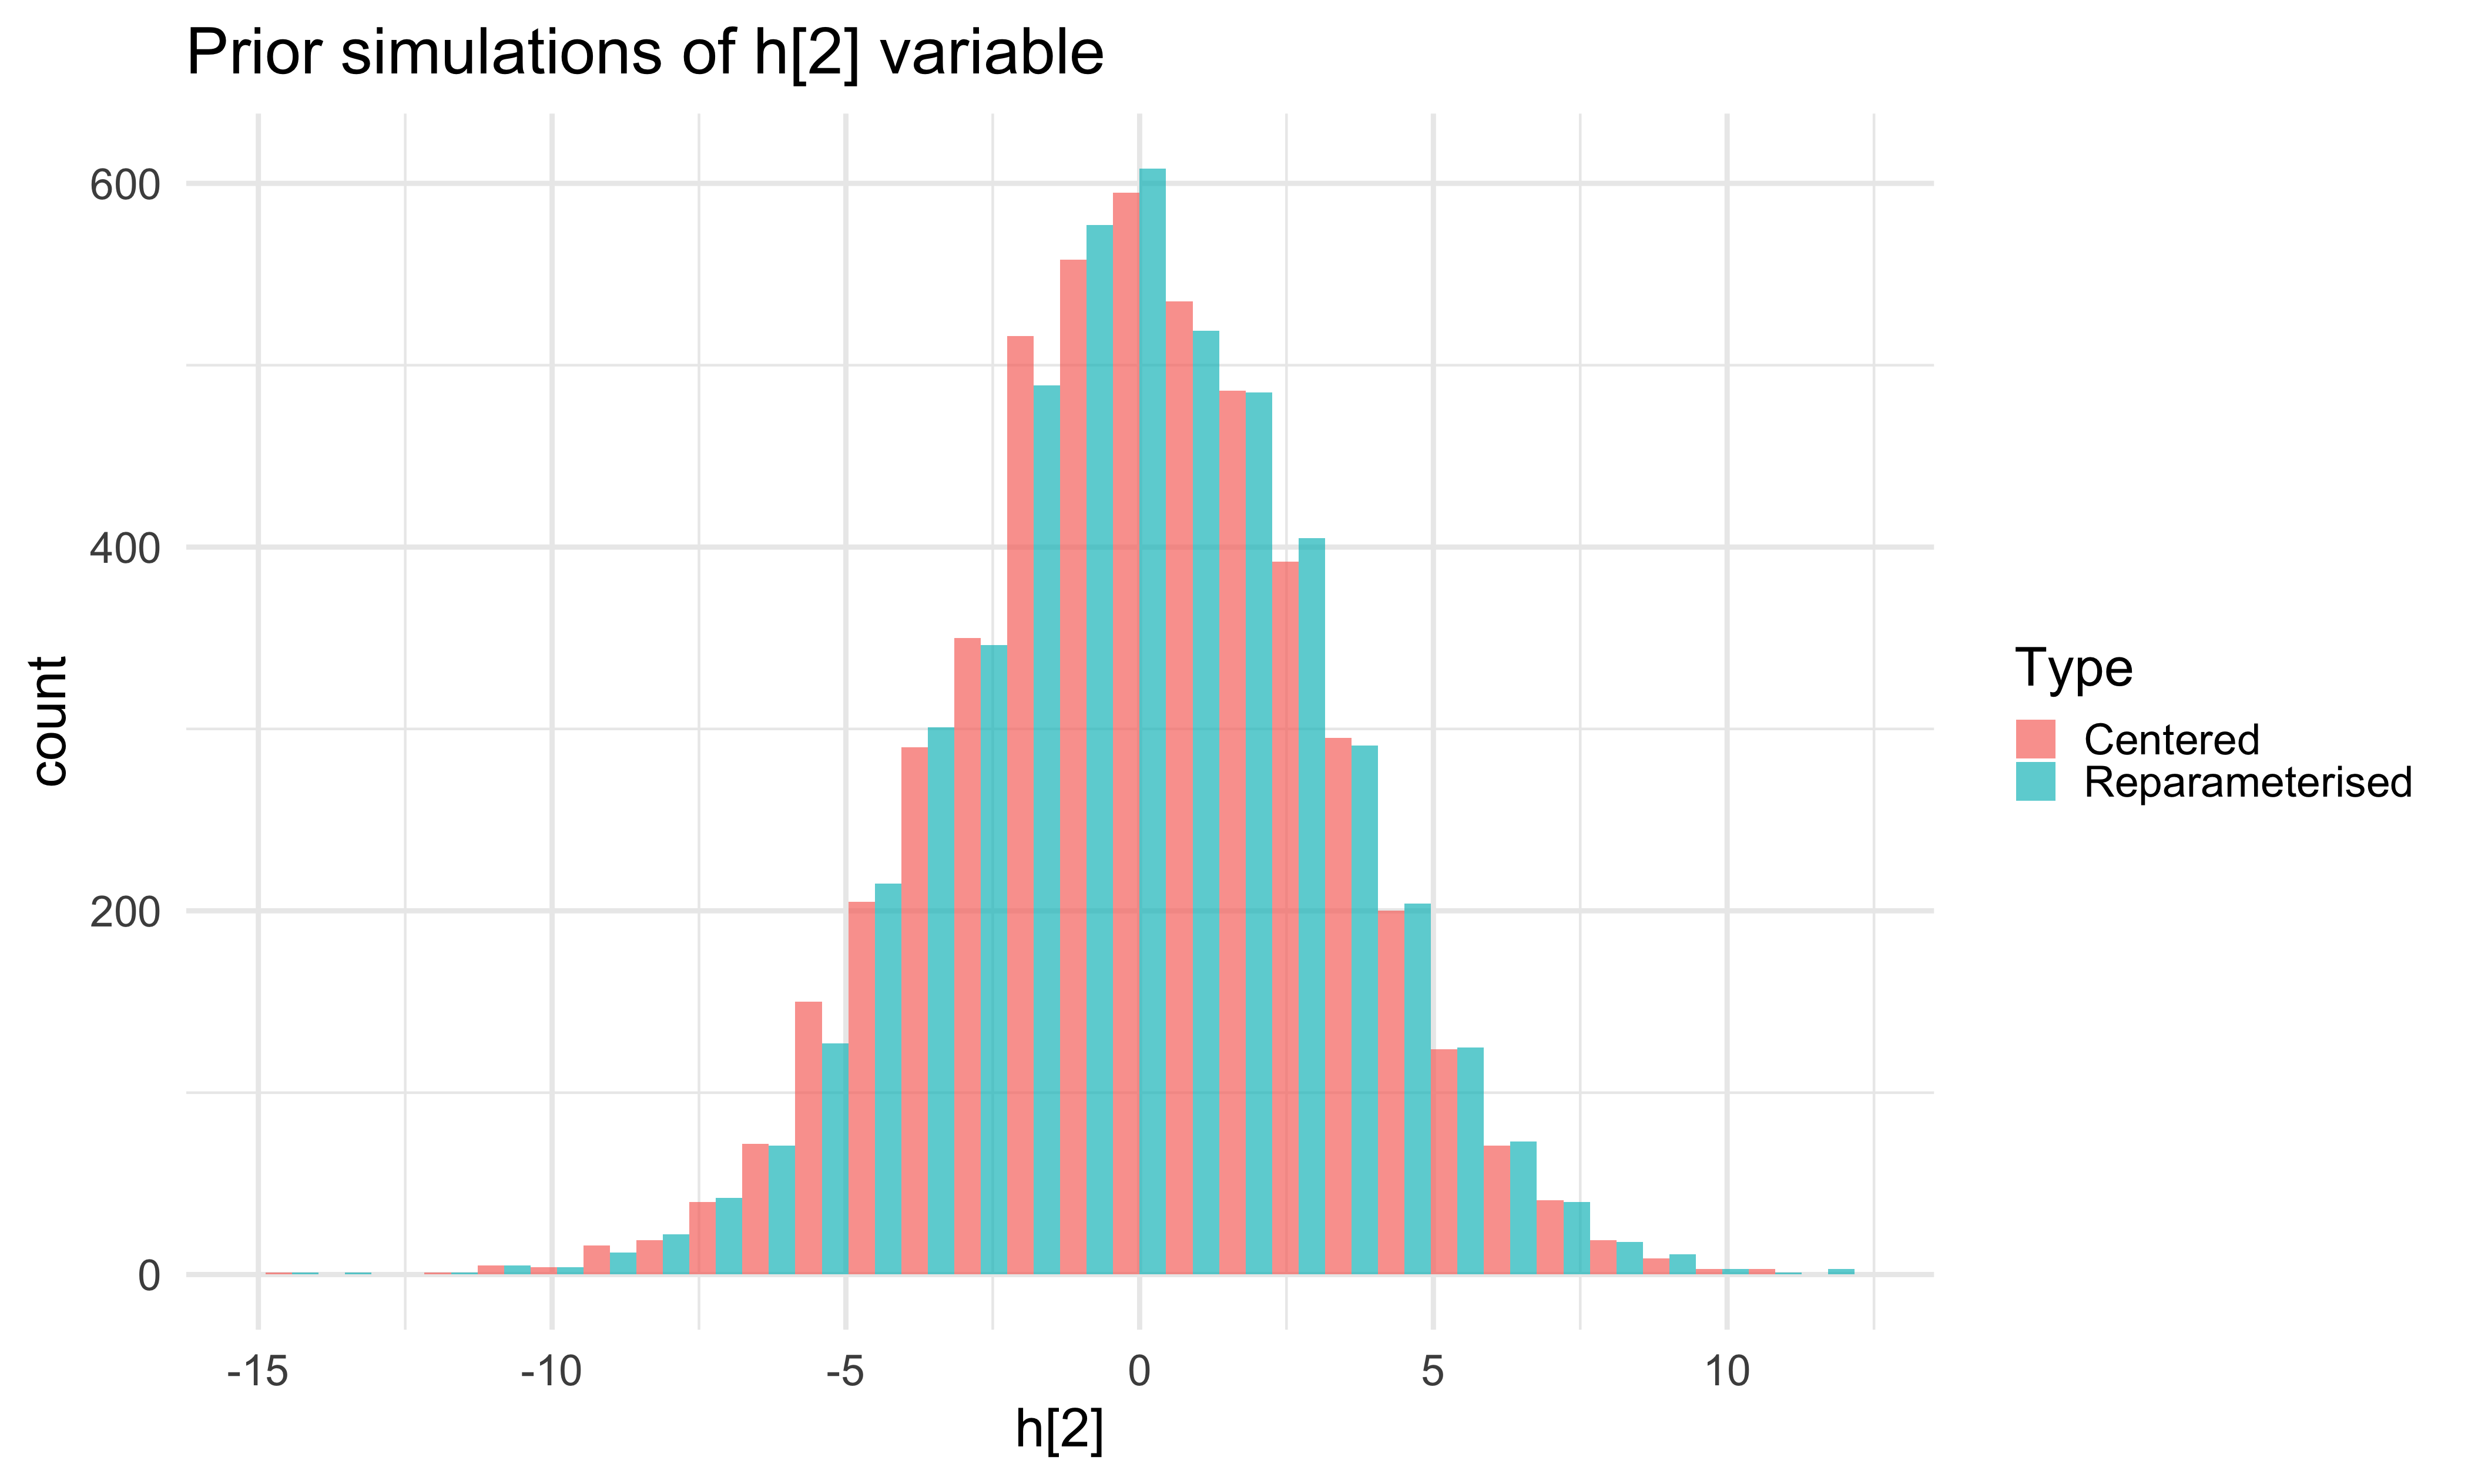
\includegraphics[scale=0.1]{figures/ppc_h2.png}
            \caption{Prior predictive samples of second state variable}
        \end{figure}
        
        % Emphasise here that different paramterisations of the models are the same model
        % Use a prior predictive check from both paramterisations show that the results are
        % the same


\section{Results}
    1000 and 5000 SBC iterations are run for centered and reparameterised versions of the stocashtic volatility model. Rank statistics histograms are presented for the static parameters and the 1st, 500th and 1000th latent state parameters with 20 bins constructed for each parameter. The black horizontal line represents uniformity conditional on the number of bins and SBC iterations. The $\chi^2$ statistic is used to summarise the deviations from uniformity for all parameters since it is unrealistic to visually inspect all the histograms. The SBC algorithm is summarised below:

    1) for sim in 1000 iterations:
        2) Draw from prior: $\theta^{sim}\sim\pi (\theta)$
        3) Simulate dataset with 1000 observations: $y^{sim} \sim p(y|\theta^{sim})$
        4) Draw 999 posterior samples (post warmup) $\{\theta_1,\dots , \theta_{L}\} \sim p(\theta | y^{sim})$
        5) Compute rank statistics $r = rank(\{\theta_1,\dots , \theta_{L}\}, \theta^{sim})$
        
    \subsection{Hamiltonian Monte Carlo}
    Figure \ref{fig:cphmc1k} and Figure \ref{fig:ncphmc1k} show the SBC results for the centered and reparameterisd model for HMC respectively. Both sets of results display relatively noisy rank statistic estimates with variation around the discrete uniform distribution.

    The centered parameterisation in particular displays a lack of uniformity for $\phi$ and $\sigma^2$. Rank statistics for $\sigma^2$ show two peaks of either end of the histogram and a left peak for $phi$. Posterior estimates of $\sigma^2$ are \textit{underdispersed} relative to the true parameter $\sigma^2_{sim}$ generated by the prior distribution. On the other hand, the posterior samples of $\phi$ are \textit{over estimating} the true parameter generated by the prior. This suggests the posterior geometry for these parameters (at least) are difficult to sample for the HMC algorithm.

    \begin{figure}[H]
        \centering
        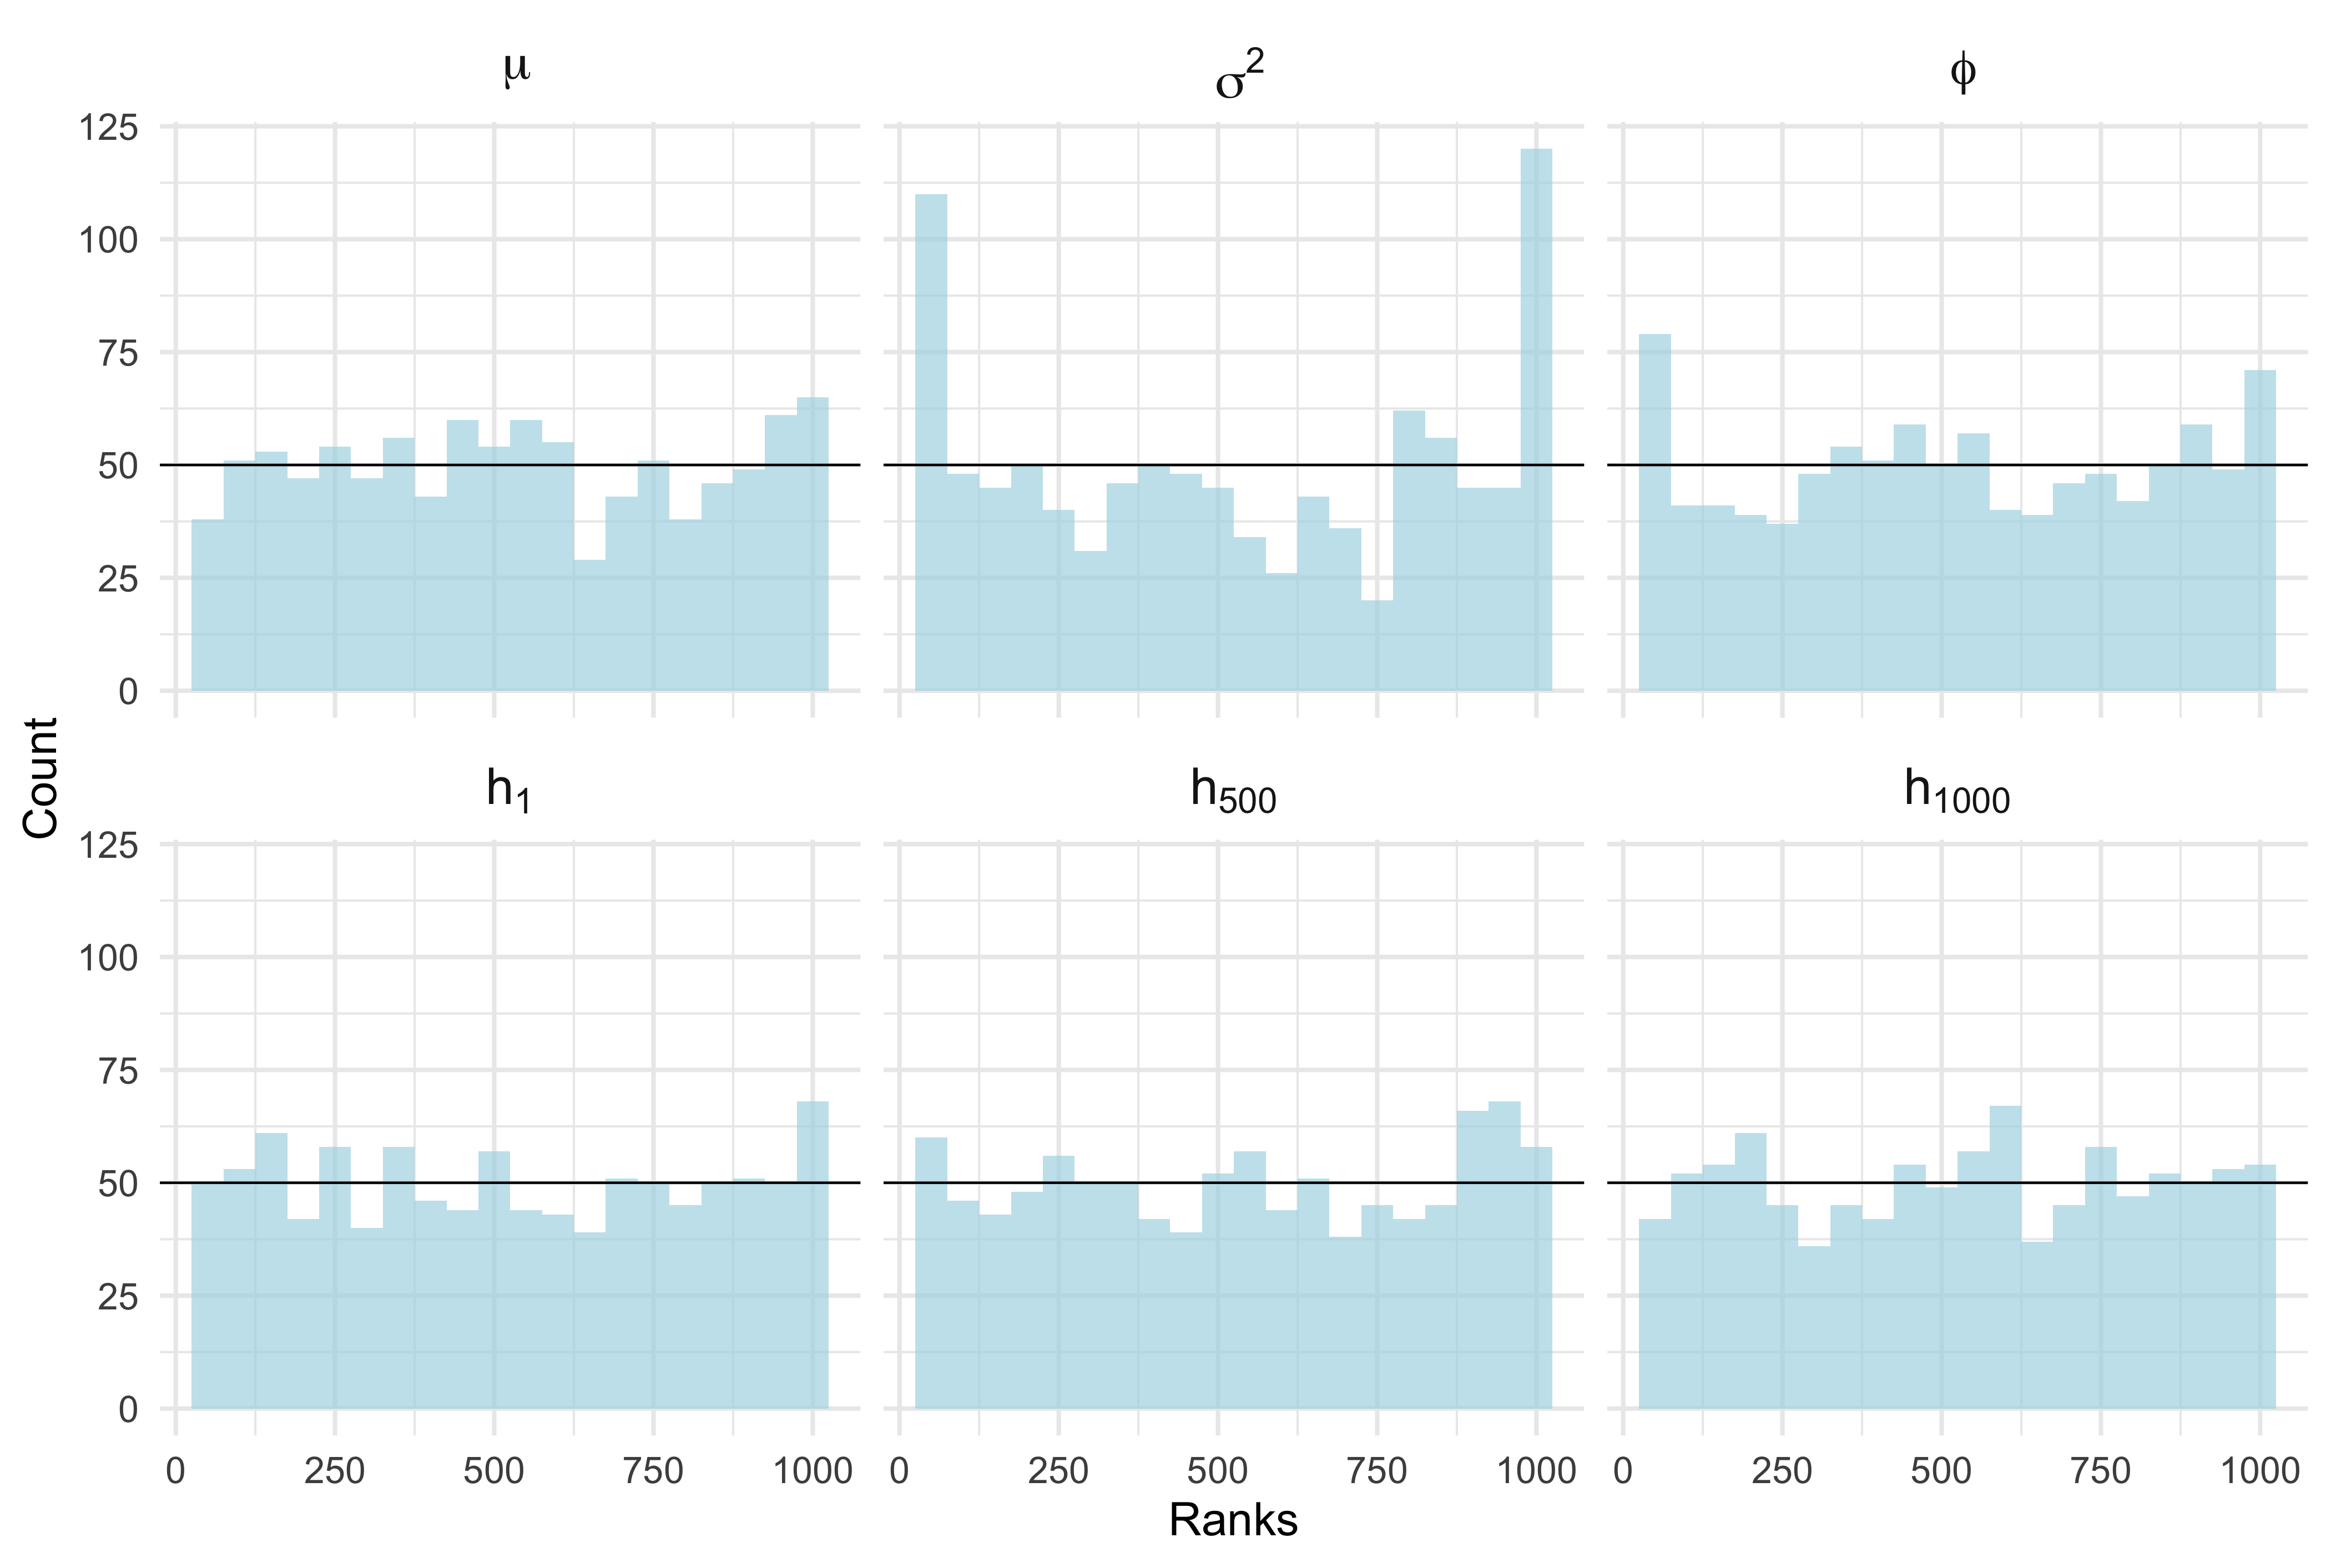
\includegraphics[scale=0.09]{results/hmc_cp_1k.png}
        \caption{1000 SBC iterations for centered model using Hamiltoninan Monte Carlo. Histograms show noisy estimates around uniform distribution. In particular, $\sigma^2$ displays peaks on both ends of the histogram and $\phi$ shows a major on the left hand side. This suggests that the posterior samples of $\sigma^2$ are underdispersed relative to the prior distribution and posterior samples of $\phi$ are over estimating the true parameter.}
        \label{fig:cphmc1k}
    \end{figure}

    Estimates of $\sigma^2$ and $\phi$ are more uniform under the reparameterised model. Instead, we observe a peak on the left side for the 500th state parameter $h_{500}$. Overall the estimates for non centered parameterisation are more favourable. 

    \begin{figure}[H]
        \centering
        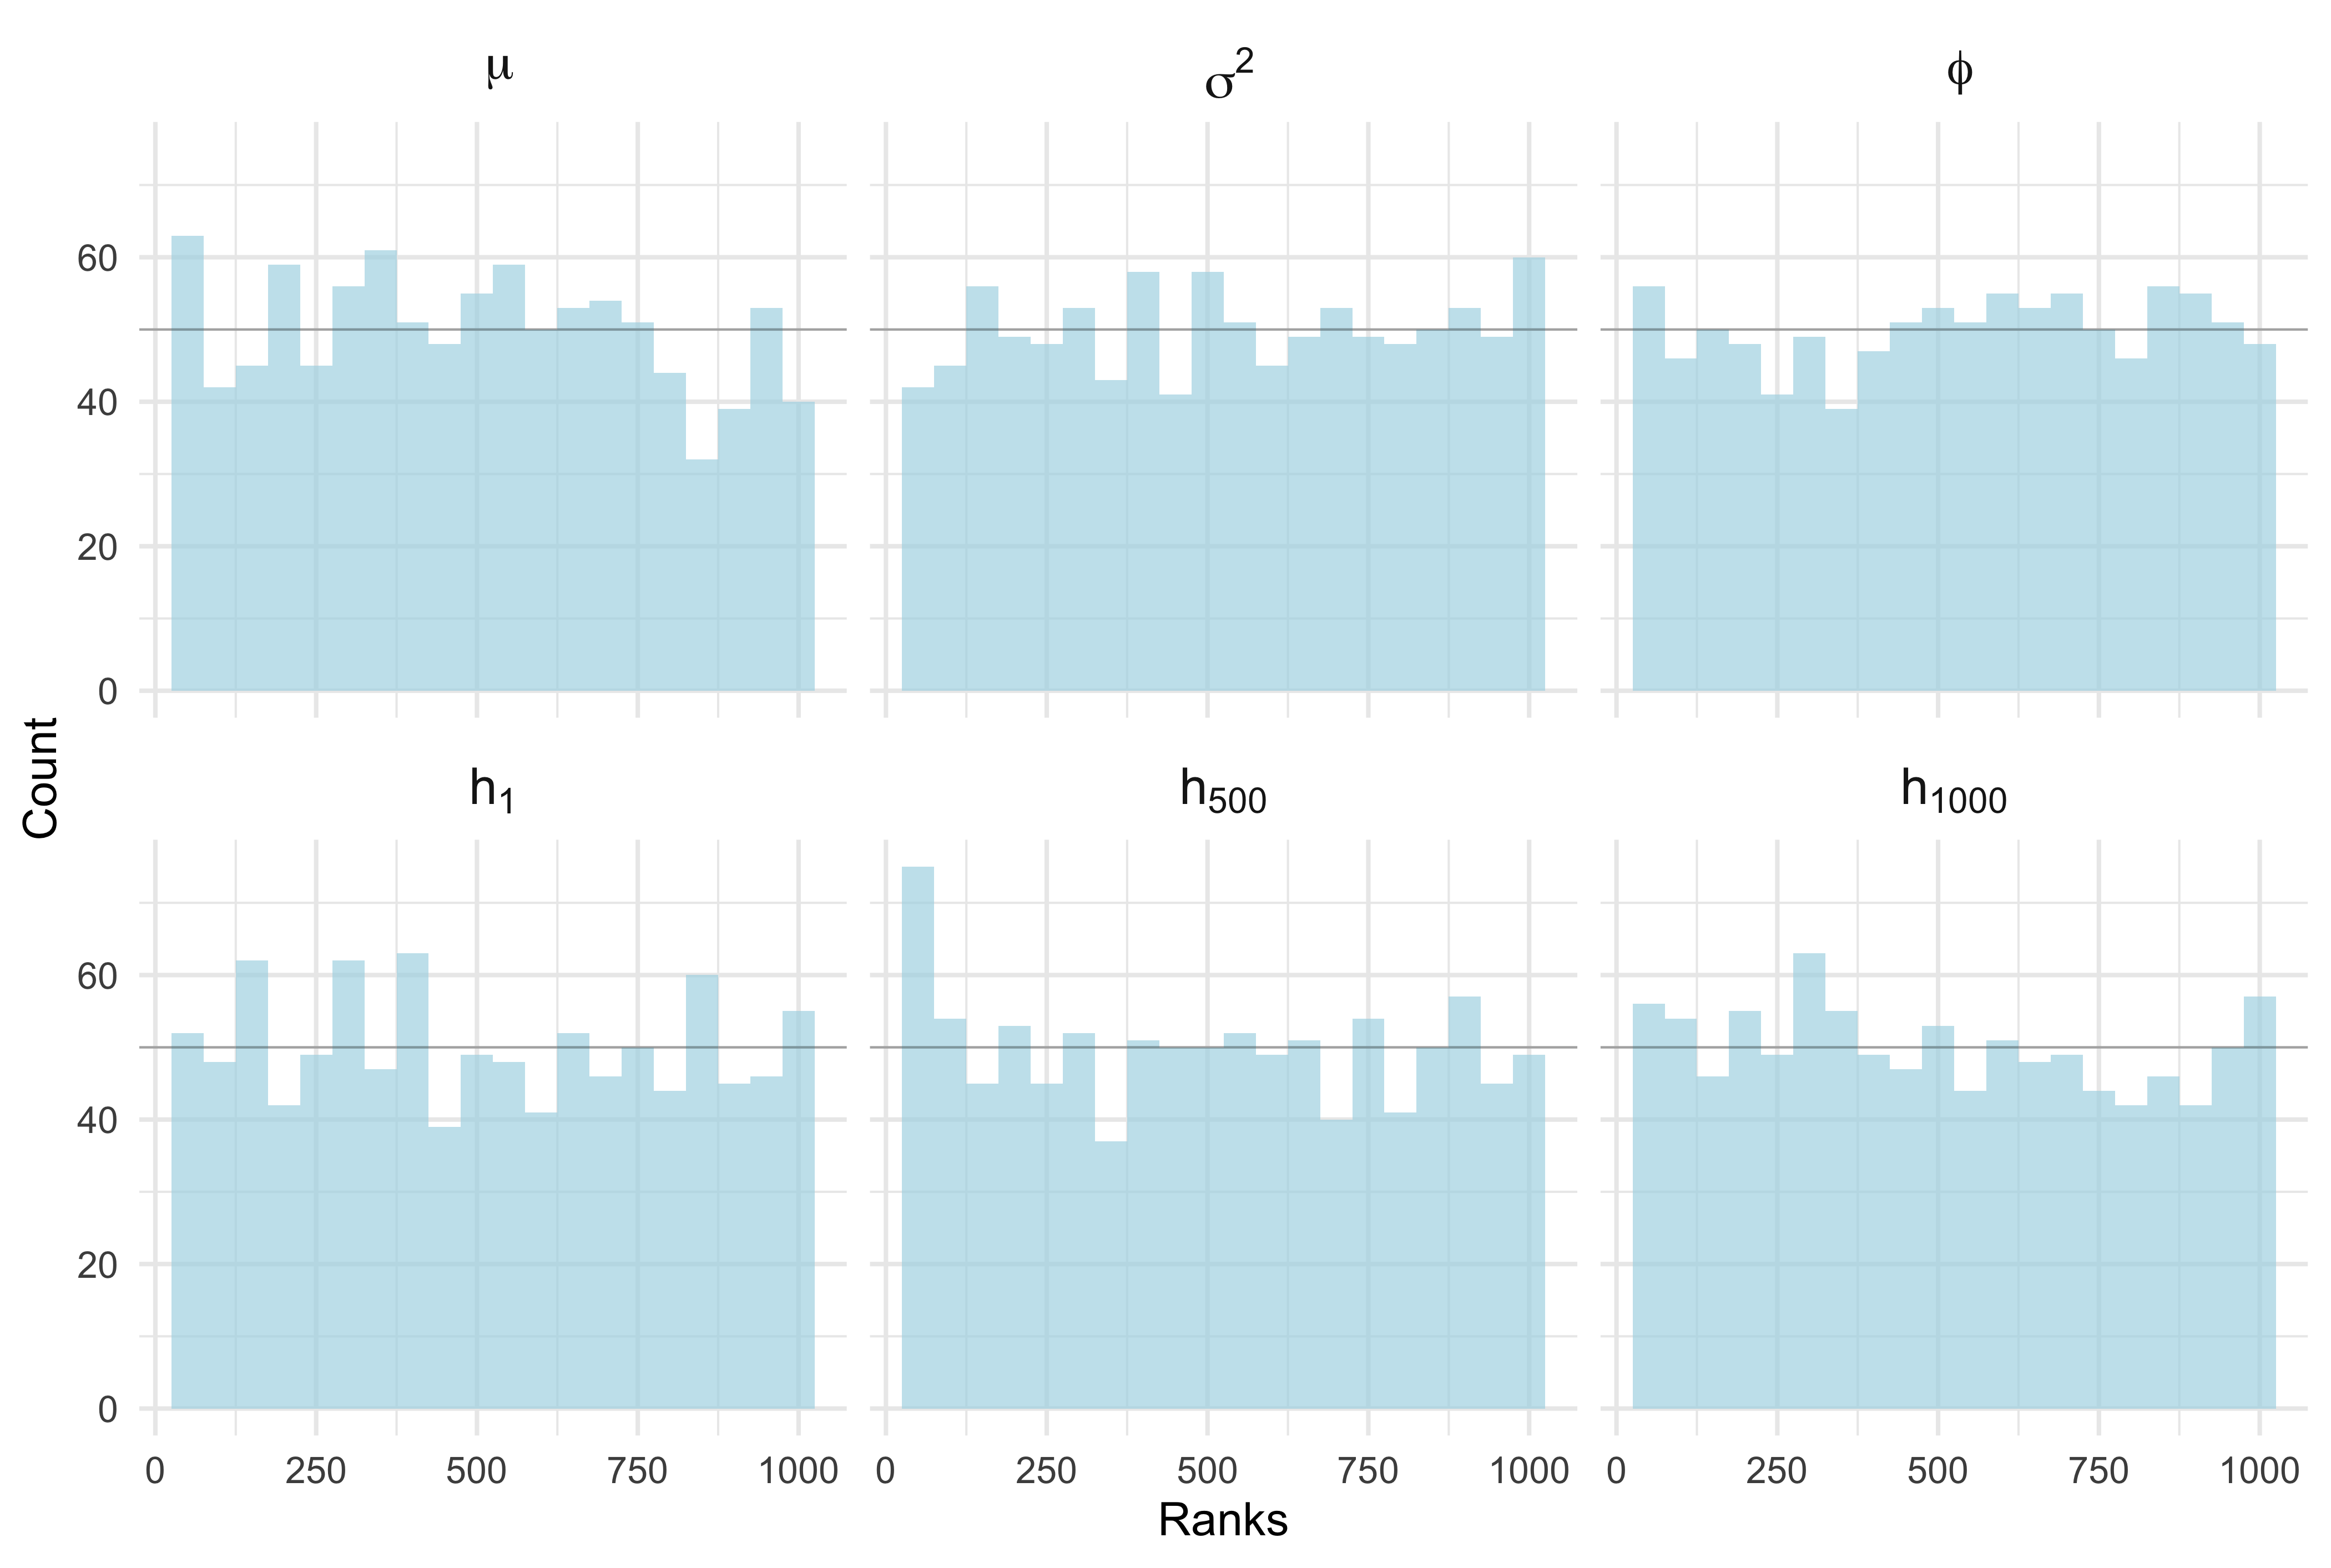
\includegraphics[scale=0.09]{results/hmc_ncp_1k.png}
        \caption{1000 SBC iterations for non centered model using Hamiltonian Monte Carlo. The rank statistic distributions for $\sigma^2$ and $\phi$ have improved. There is some evidence of over estimation of the 500th state parameter.}
        \label{fig:ncphmc1k}
    \end{figure}

    The noisy histogram estimates can be improved by increasing the number of SBC iterations. Figure \ref{fig:cphmc5k} and Figure \ref{fig:ncphmc5k} show the results of the same parameters with 5000 SBC iterations. There is an improvement to the reparameterised model with all histograms looking approximately uniform with much smaller variation around the true uniform value. 
    
    Centered parameteristion posess similar improvement for $\mu$ and the state parameters. However, there are still major peaks at both ends of $\sigma^2$ and $\phi$ suggesting underdispersion of the posterior estimates relative to the prior distribution.

    These results suggests that HMC overall struggles to sample from the centered parameteristion of the stochastic volatility model. The reparameterised model results in much better and consistent inference for this sampling strategy, conditional on the model. 

    \begin{figure}[H]
        \centering
        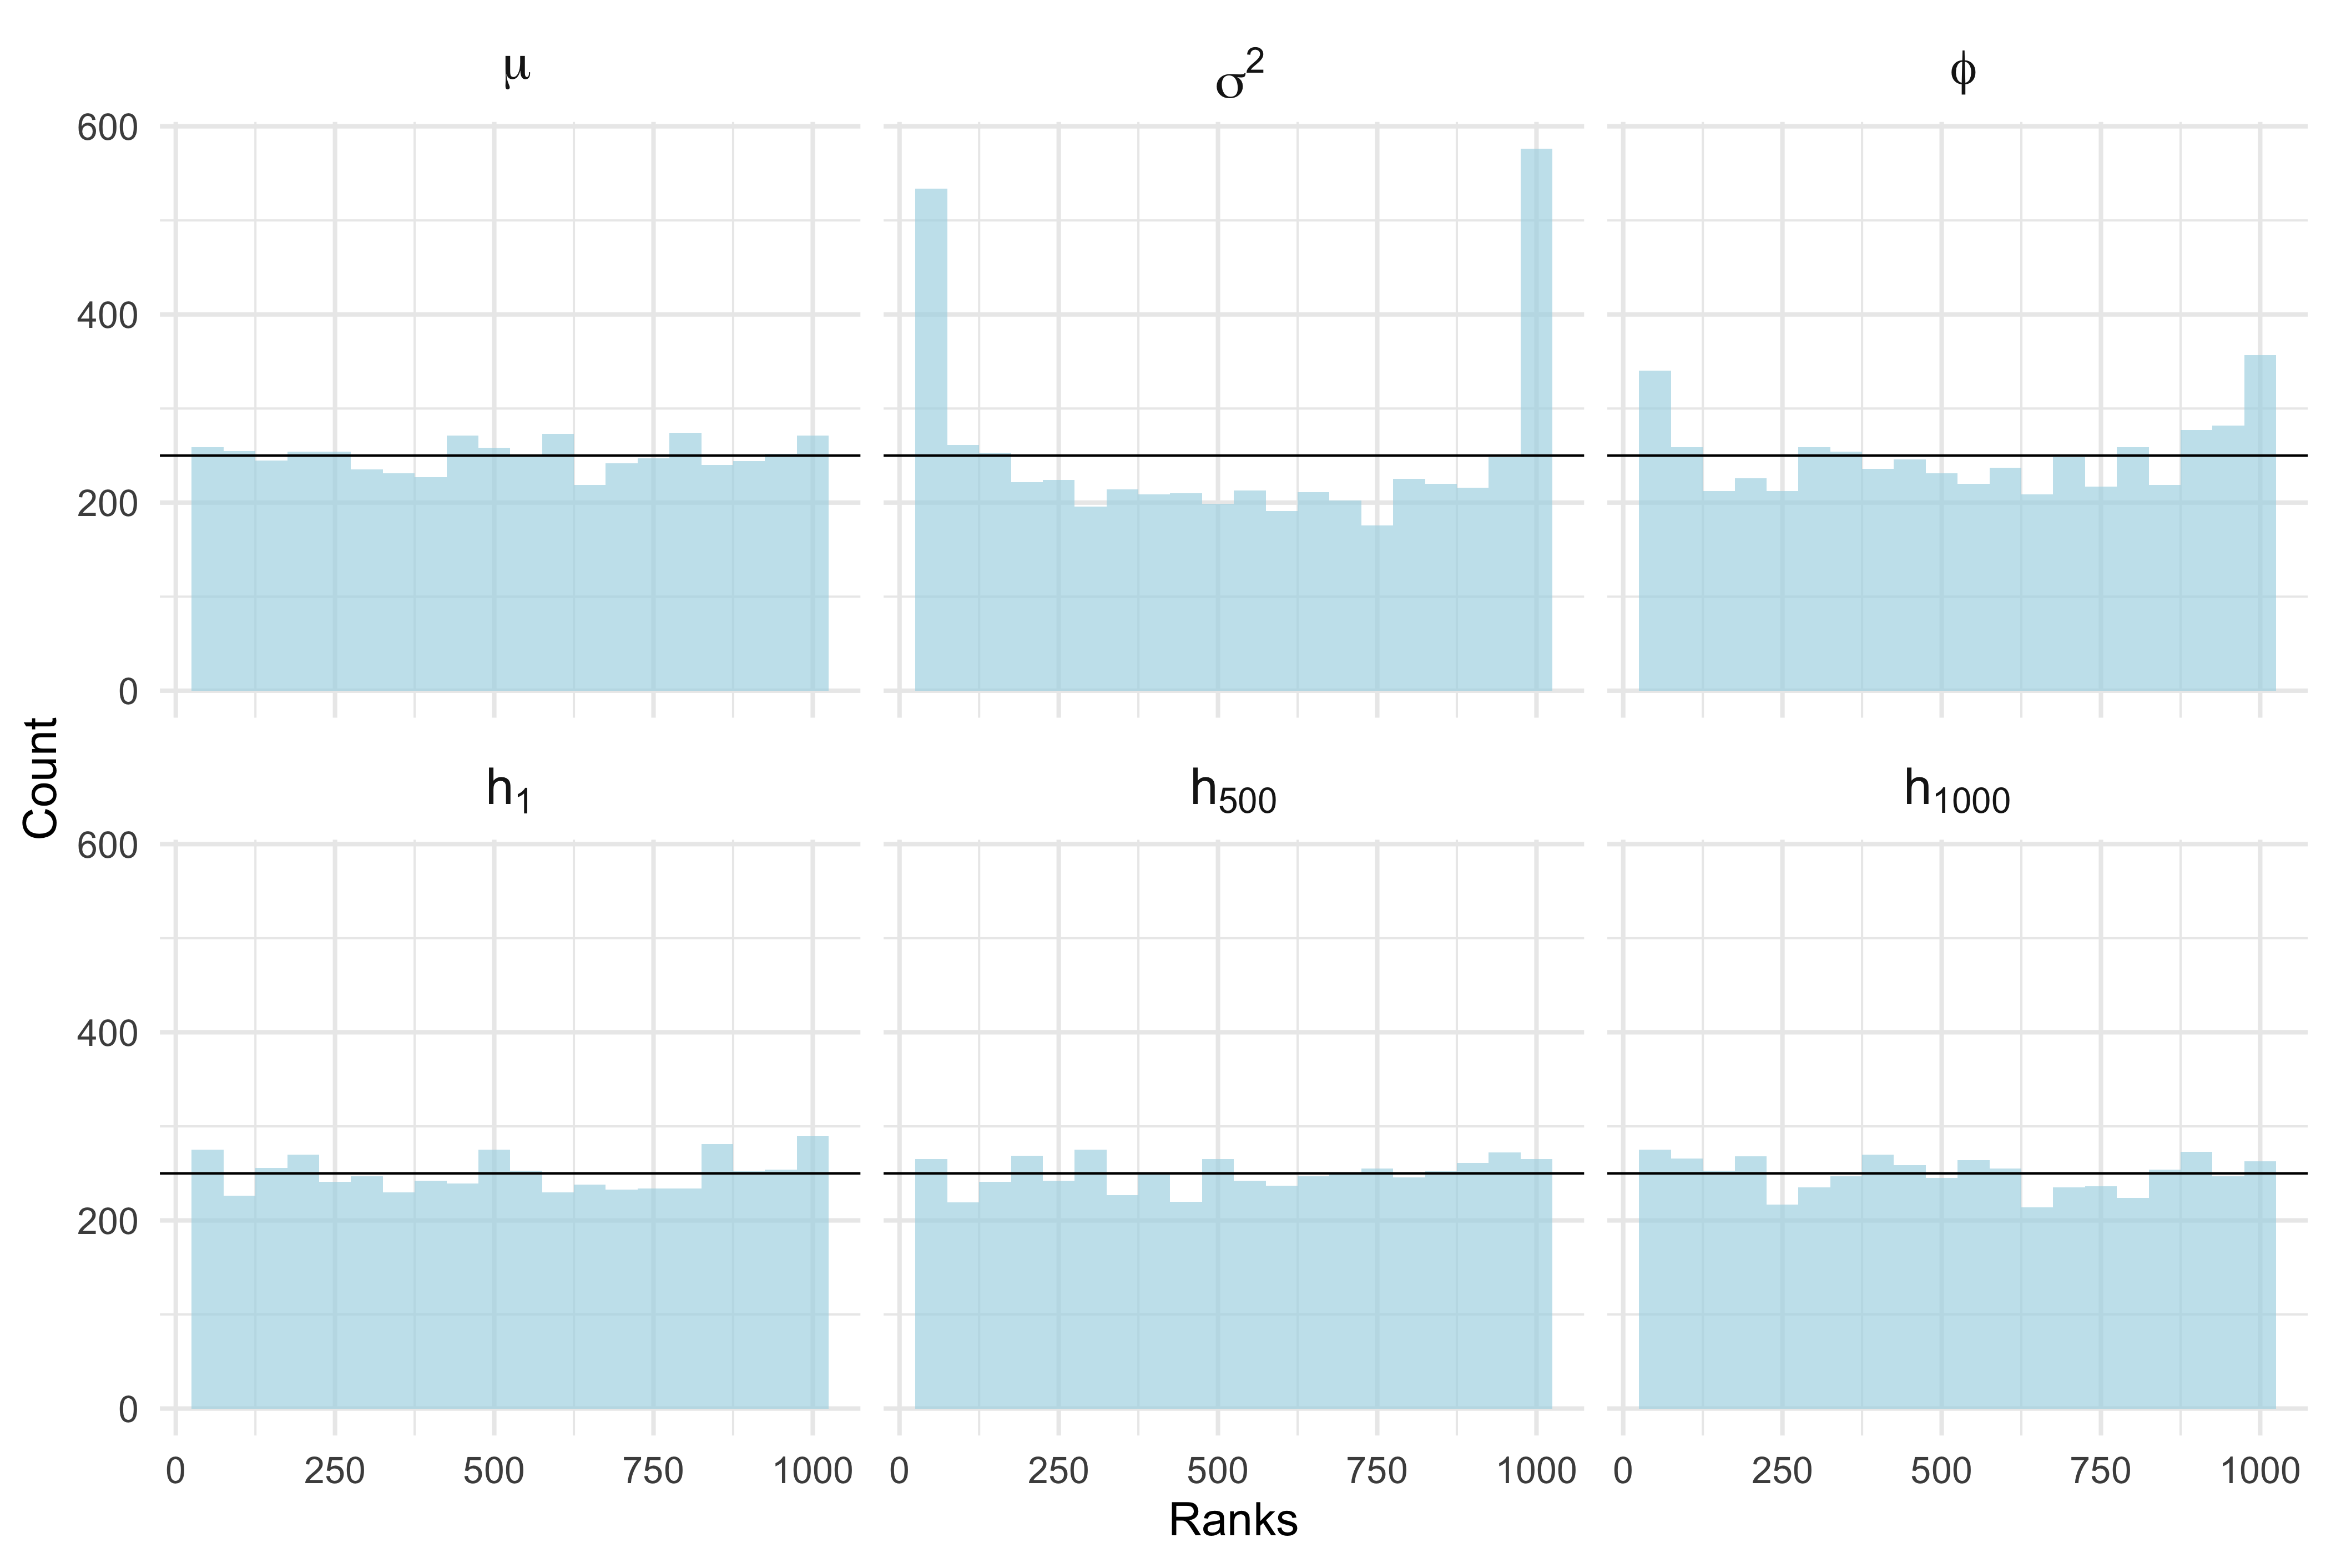
\includegraphics[scale=0.09]{results/hmc_cp_5k.png}
        \caption{5000 SBC iterations for centered model using Hamiltoninan Monte Carlo. $\mu$ and the state parameters look approximately uniform. $\sigma^2$ still has major peaks on both the left and right hand side indicating underdispersion relative to the prior distribution. $\phi$ exhibits a similar shape to $\sigma^2$ although the peaks are much smaller.}
        \label{fig:cphmc5k}
    \end{figure}

    \begin{figure}[H]
        \centering
        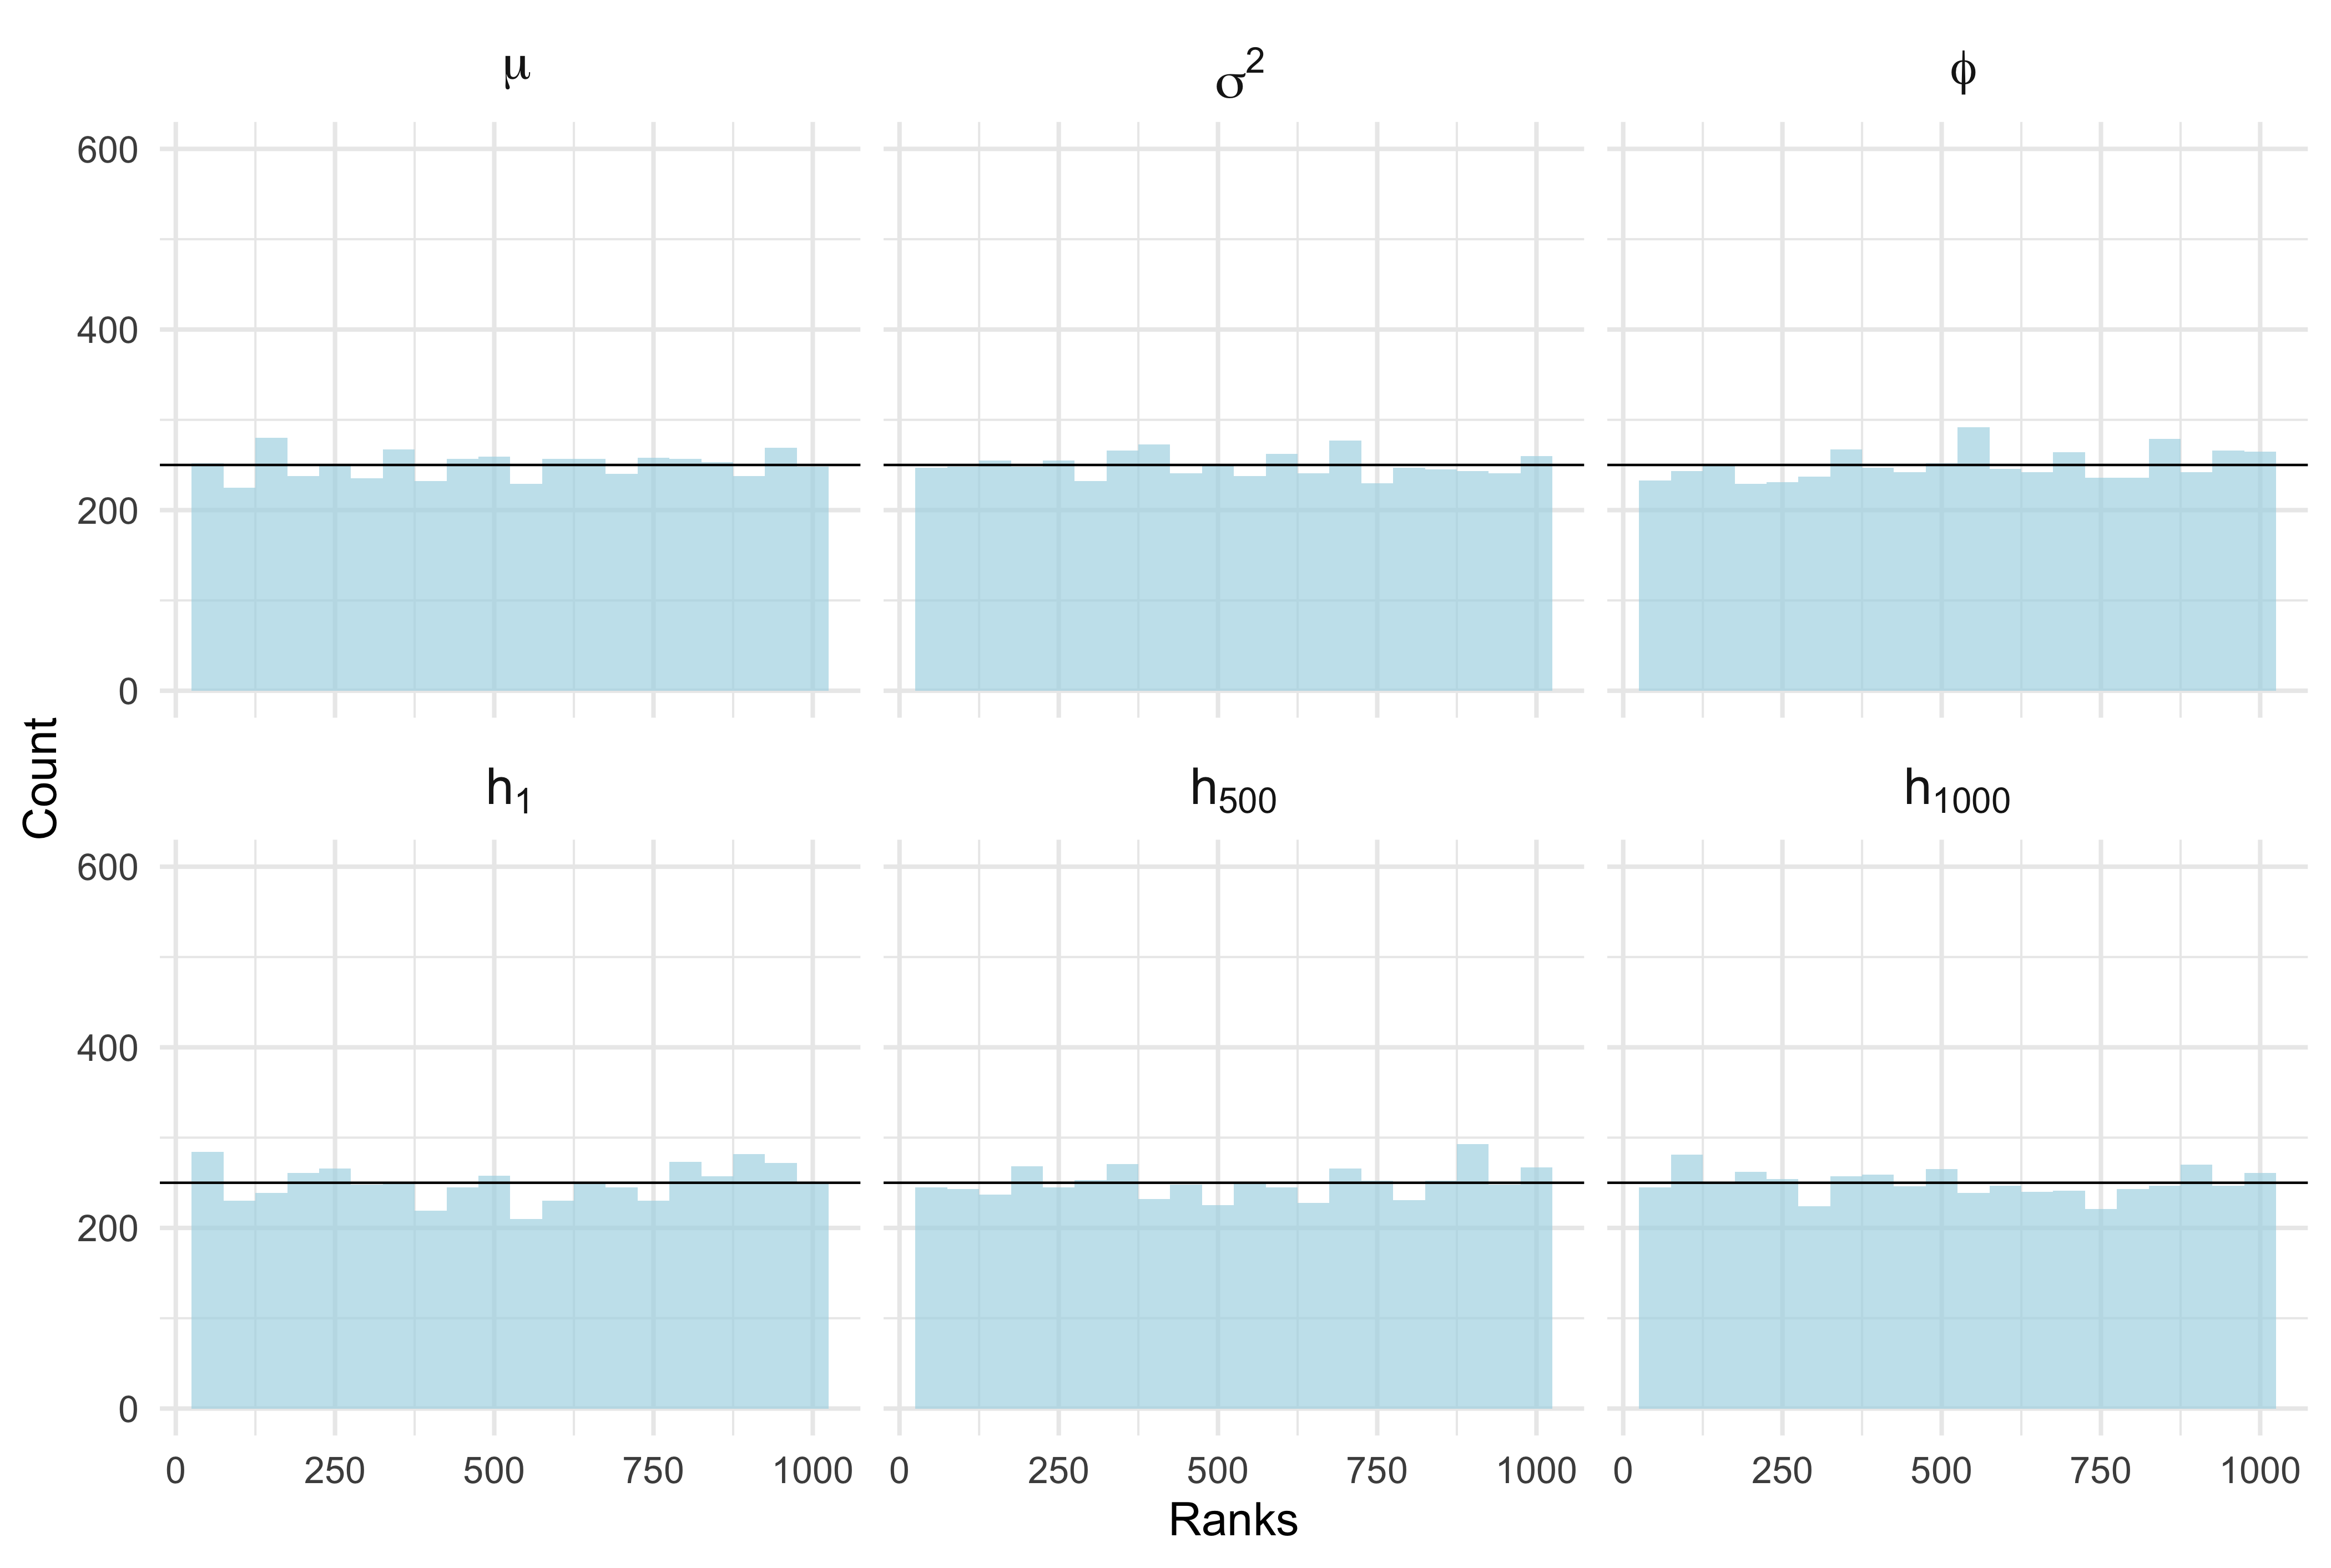
\includegraphics[scale=0.09]{results/hmc_ncp_5k.png}
        \caption{5000 SBC iterations for reparameterised model using Hamiltoninan Monte Carlo. Parameters display uniformity with less noise around the true uniform value. This suggests that the HMC algorithm is returning the correct posterior estimates for the selected parameters.}
        \label{fig:ncphmc5k}
    \end{figure}

    Further to calibration, the HMC algorithm struggles to efficiently generate posterior samples from the centered parameterisation of stochastic volatility. Figure \ref{fig:hmcess} visualises the distribution of ESS for the static parameters after 5000 SBC iterations. The non centered model appears to generate independent samples much more efficiently than the centered model. This is consistent with HMC struggliing to sample overall from the posteriors of $\sigma^2$ and $\phi$.

    \begin{figure}[H]
        \centering
        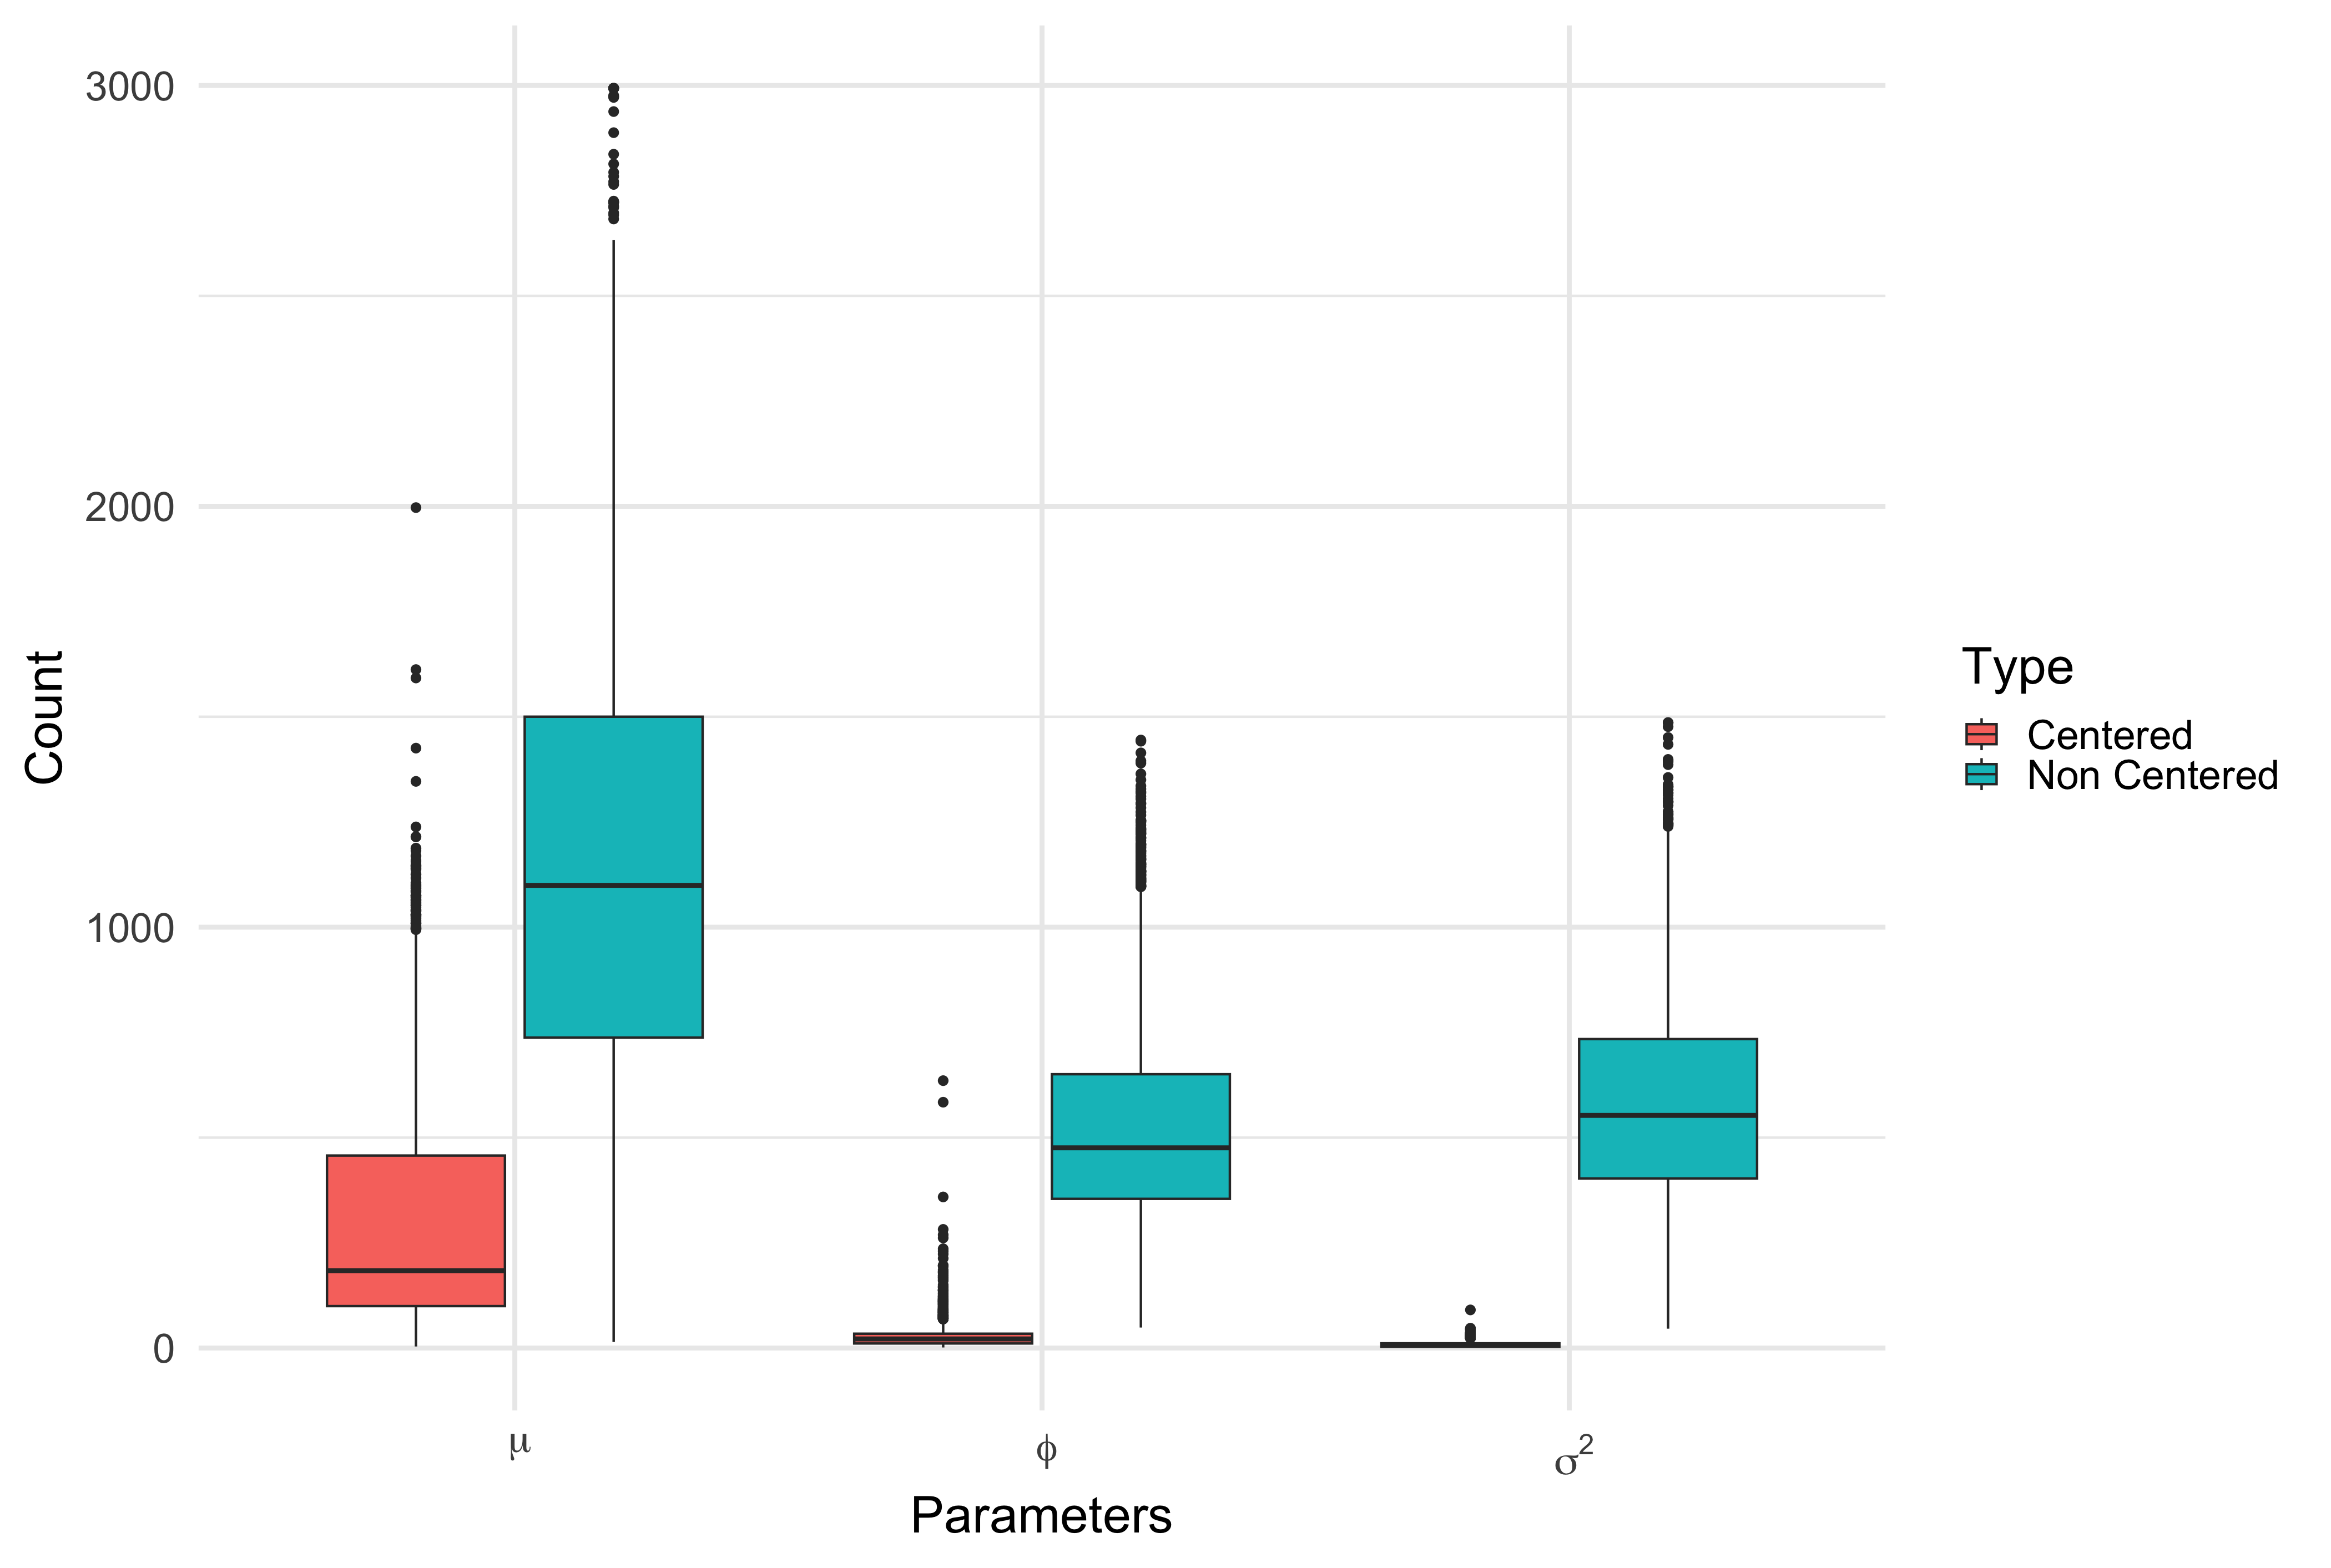
\includegraphics[scale=0.09]{results/hmc_ess.png}
        \caption{Effective sample sizes for static parameters after 5000 iterations of SBC and 1000 post warmup samples for Hamiltoninan Monte Carlo. The centered parameterisation struggles to generate independent samples for $\sigma^2$ and $\phi$. Non parameterisation demonstrates much more efficient sampling behaviour.}
        \label{fig:hmcess}
    \end{figure}

    \subsection{Gaussian Mixture Approximation}
    The Gaussian Mixture Approximation is run for 1000 and 5000 SBC iterations with the first 10,000 samples discarded as burnin (consistent with \citet{kim1998stochastic}). However, unlike KSC who take 750,000 posterior draws from the model, the number of posterior samples taken as part of the SBC procedure is 9,999. Taking 750,000 draws from the Gaussian mixture approximation would lead to issues given the disk space and compute time required from run SBC. Furthermore, the number of posterior samples is larger than the 999 taken for the SBC experiment run for Hamiltonian Monte Carlo. Earlier experiments attempted 999 post burn in draws for the Gaussian approximation, however there are concerns that such a short chain would not have converged onto the target posterior distribution. Therefore 9,999 draws was chosen as a compromise under both constraints. 

    The centered Gaussian mixture approximation contains issues with calibration. Figure \ref{fig:cpksc1k} presents the results from SBC where there is a lack of uniformity across all parameters. In particular, there is a large peak on the left hand side for $\mu$ and the right hand hand side of $\phi$. This suggests over estimation and under estimation of the true parameter respectively. All other parameters do not have any key features worth noting beyond noisy estimates around the true discrete uniform value. 

    \begin{figure}[H]
        \centering
        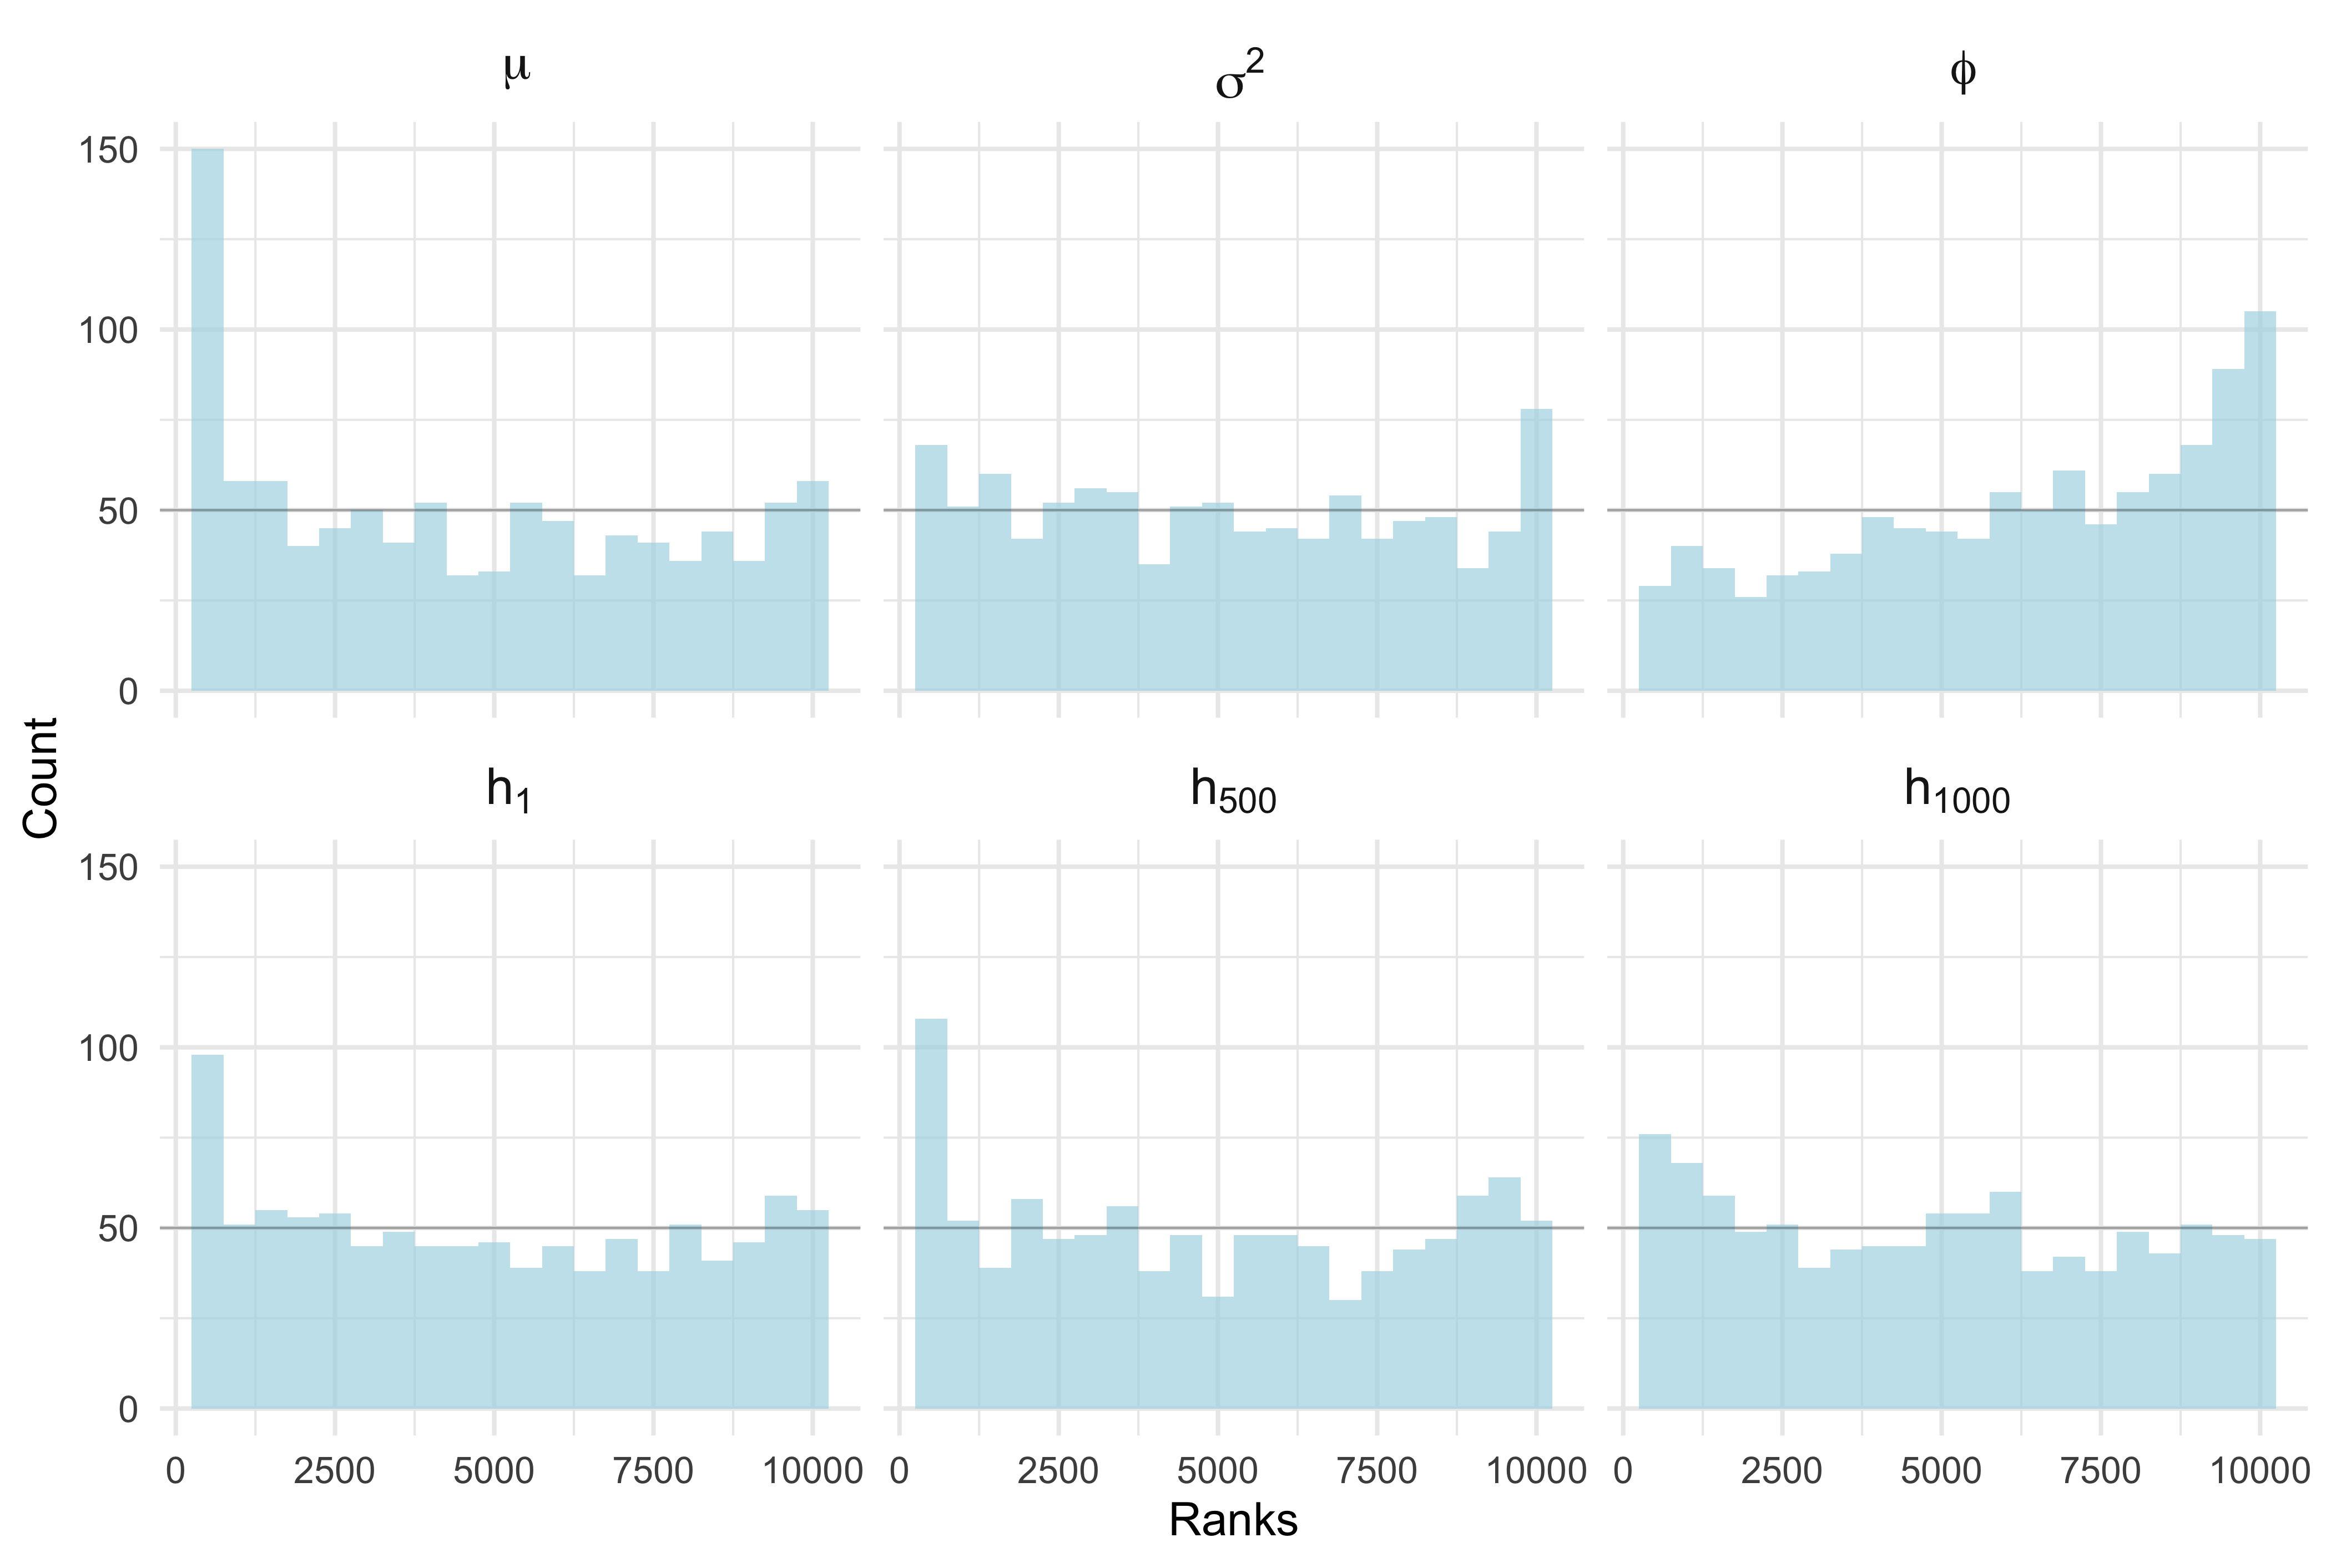
\includegraphics[scale=0.1]{results/ksc_cp_1k.png}
        \caption{1000 SBC iterations for centered Gaussian mixture approximation model. The rank statistics for all the selected parameters display a lack of uniformity. $\mu$ has a large left peak suggesting the algorithm is over estimating the true parameter. The converse can be said about $\phi$ which possesses a peak on the right hand side which implies underestimation of the true parameter.}
        \label{fig:cpksc1k}
    \end{figure}

    Increasing the SBC iterations to 5000 does not improve the results. $\sigma^2$ and the state parameters contain arguably less noisy estimates around the uniform distribution. However, the skewed shapes of $\mu$ and $\phi$ adds further evidence that the sampling strategy is not returning the correct posterior estimates. This can be seen in Figure \ref{fig:cpksc5k}.

    \begin{figure}[H]
        \centering
        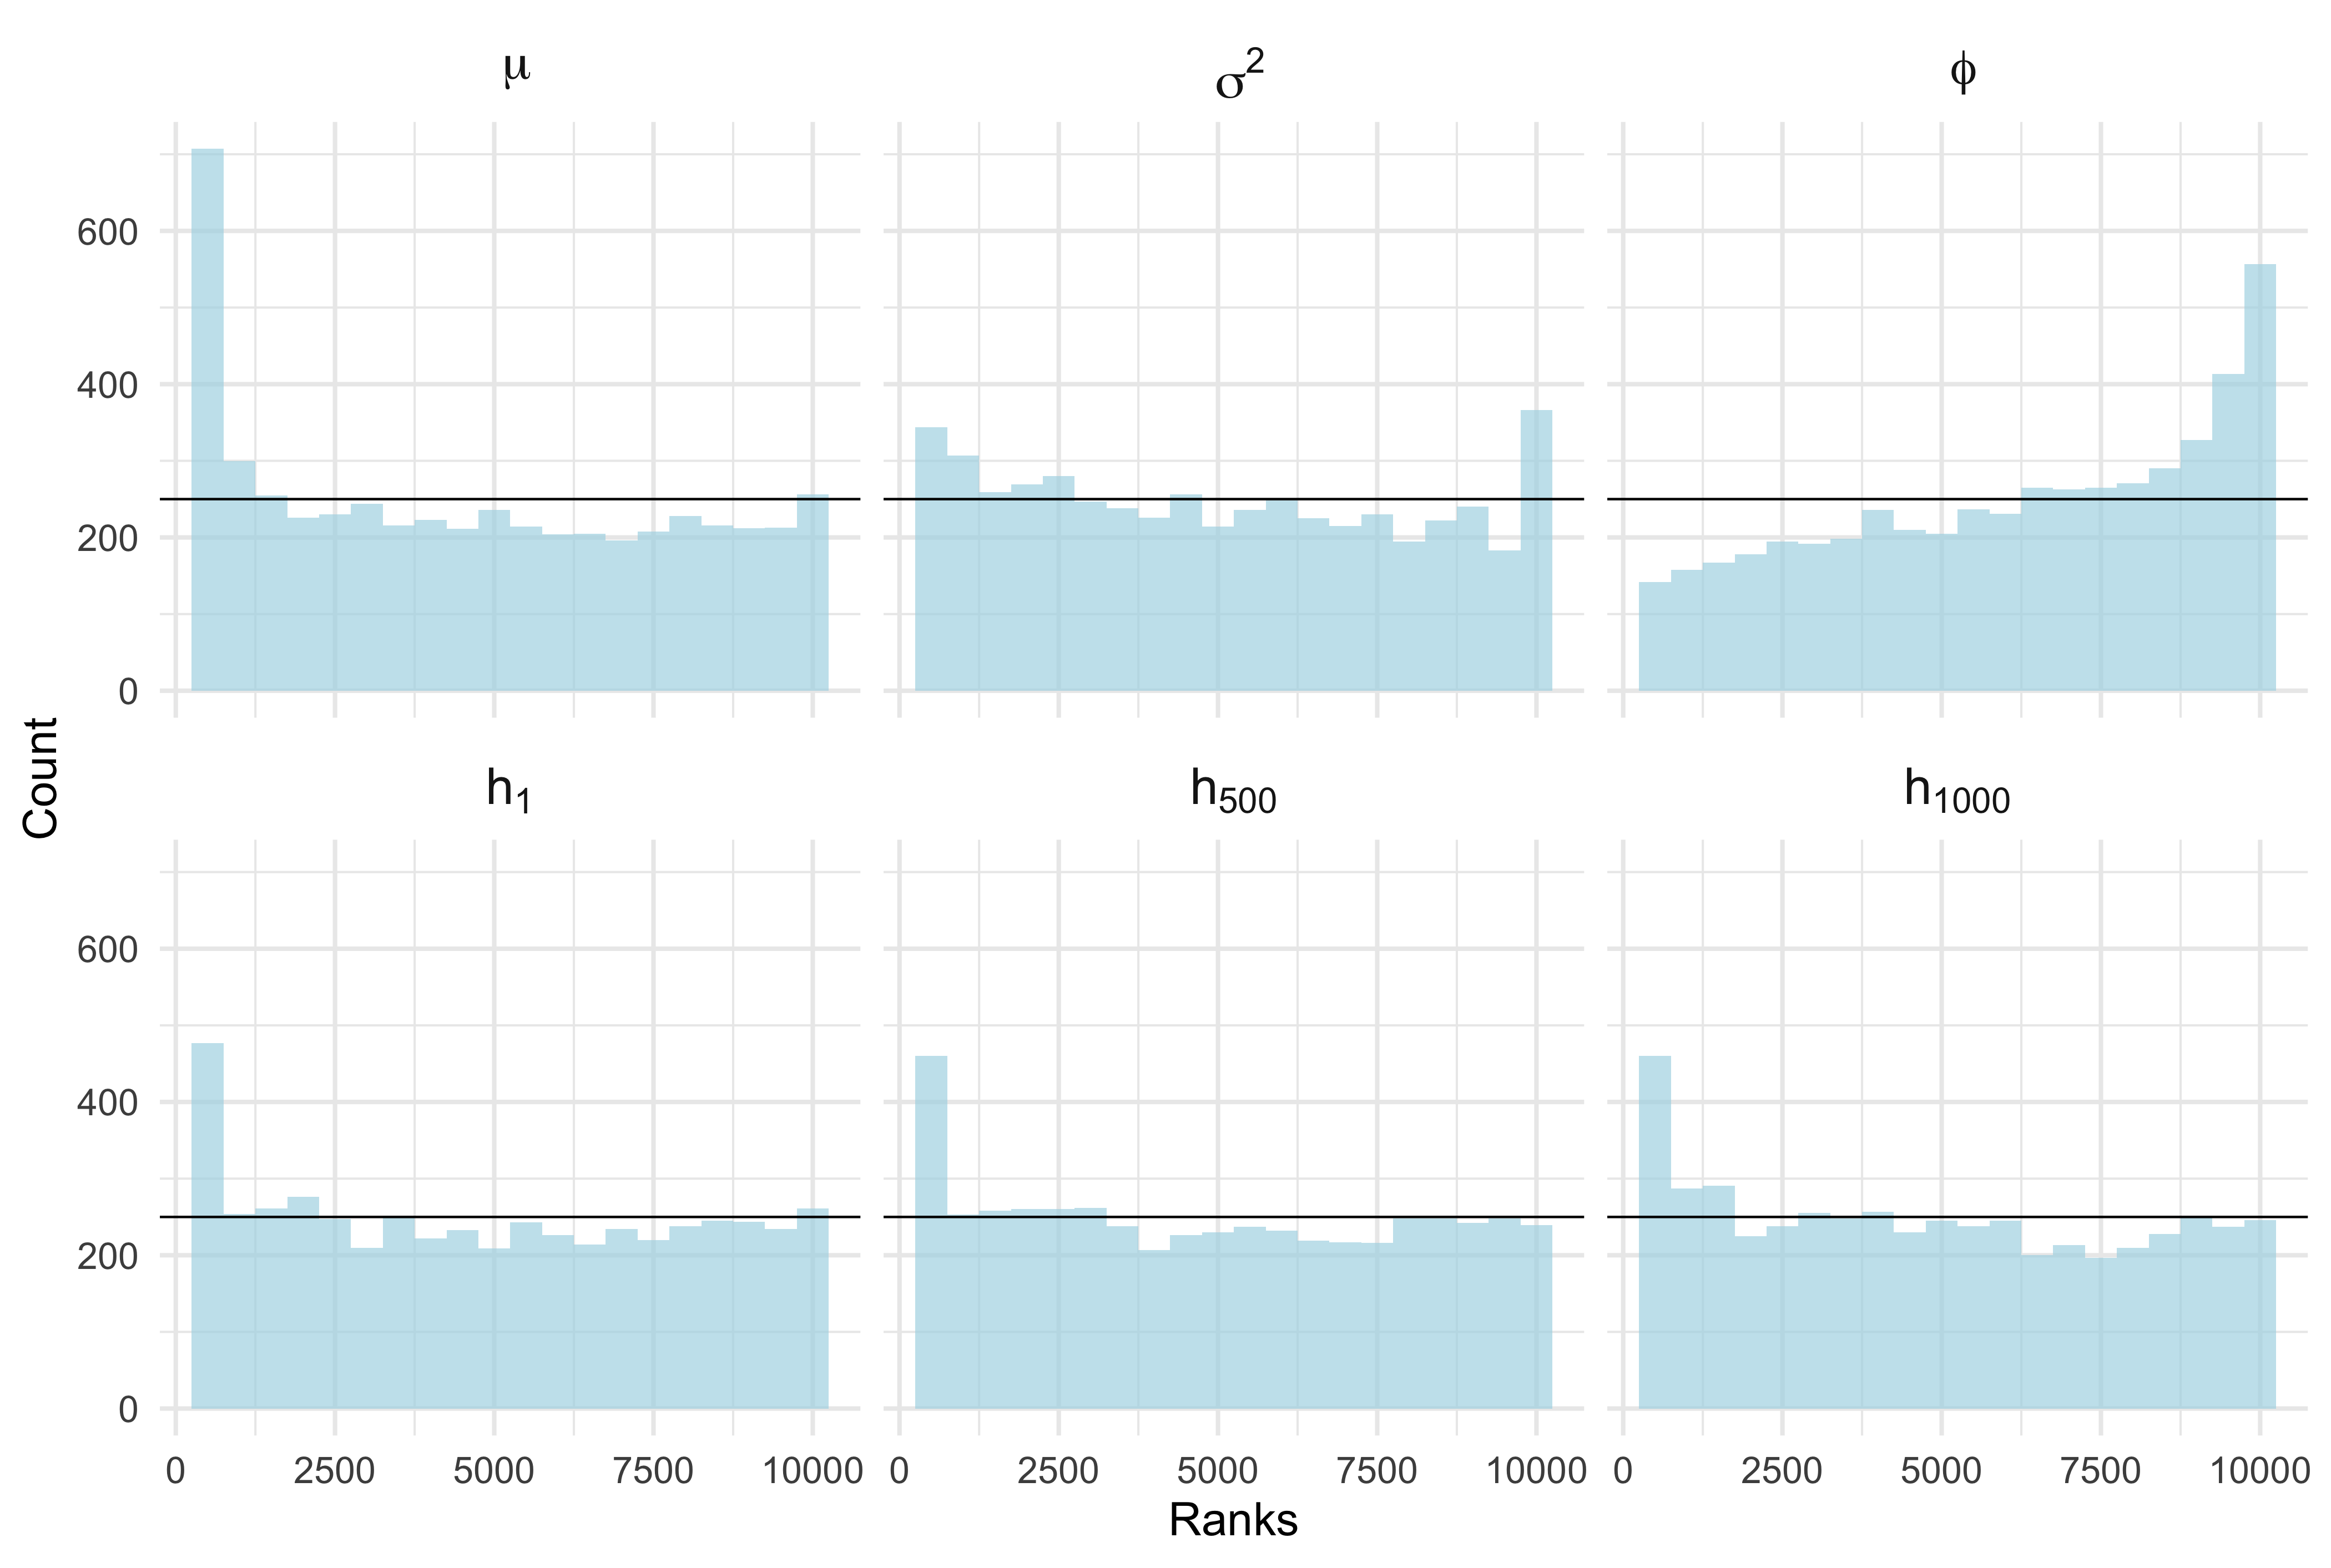
\includegraphics[scale=0.1]{results/ksc_cp_5k.png}
        \caption{5000 SBC iterations for centered Gaussian mixture approximation model. Estimates for $\sigma^2$ and the state parameters have marginally improved around the uniformity. However, there is no improvement in $\mu$ or $\phi$, suggesting a lack of calibration from the MCMC algorithm.}
        \label{fig:cpksc5k}
    \end{figure}

    Furthermore, the ESS estimates for this model indicate a high degree of autocorrelation and difficulty in generating independent samples from the posterior distribution. The median ESS for $\mu$, $\phi$ and $\sigma^2$ are 559, 103, 39.5 respectively for 10,000 post burn in draws. Despite having 10 times the number of draws, the number of effectively independent samples is much smaller relative to HMC, suggesting that this bespoke sampling strategy is highly inefficient. 

    \begin{figure}[H]
        \centering
        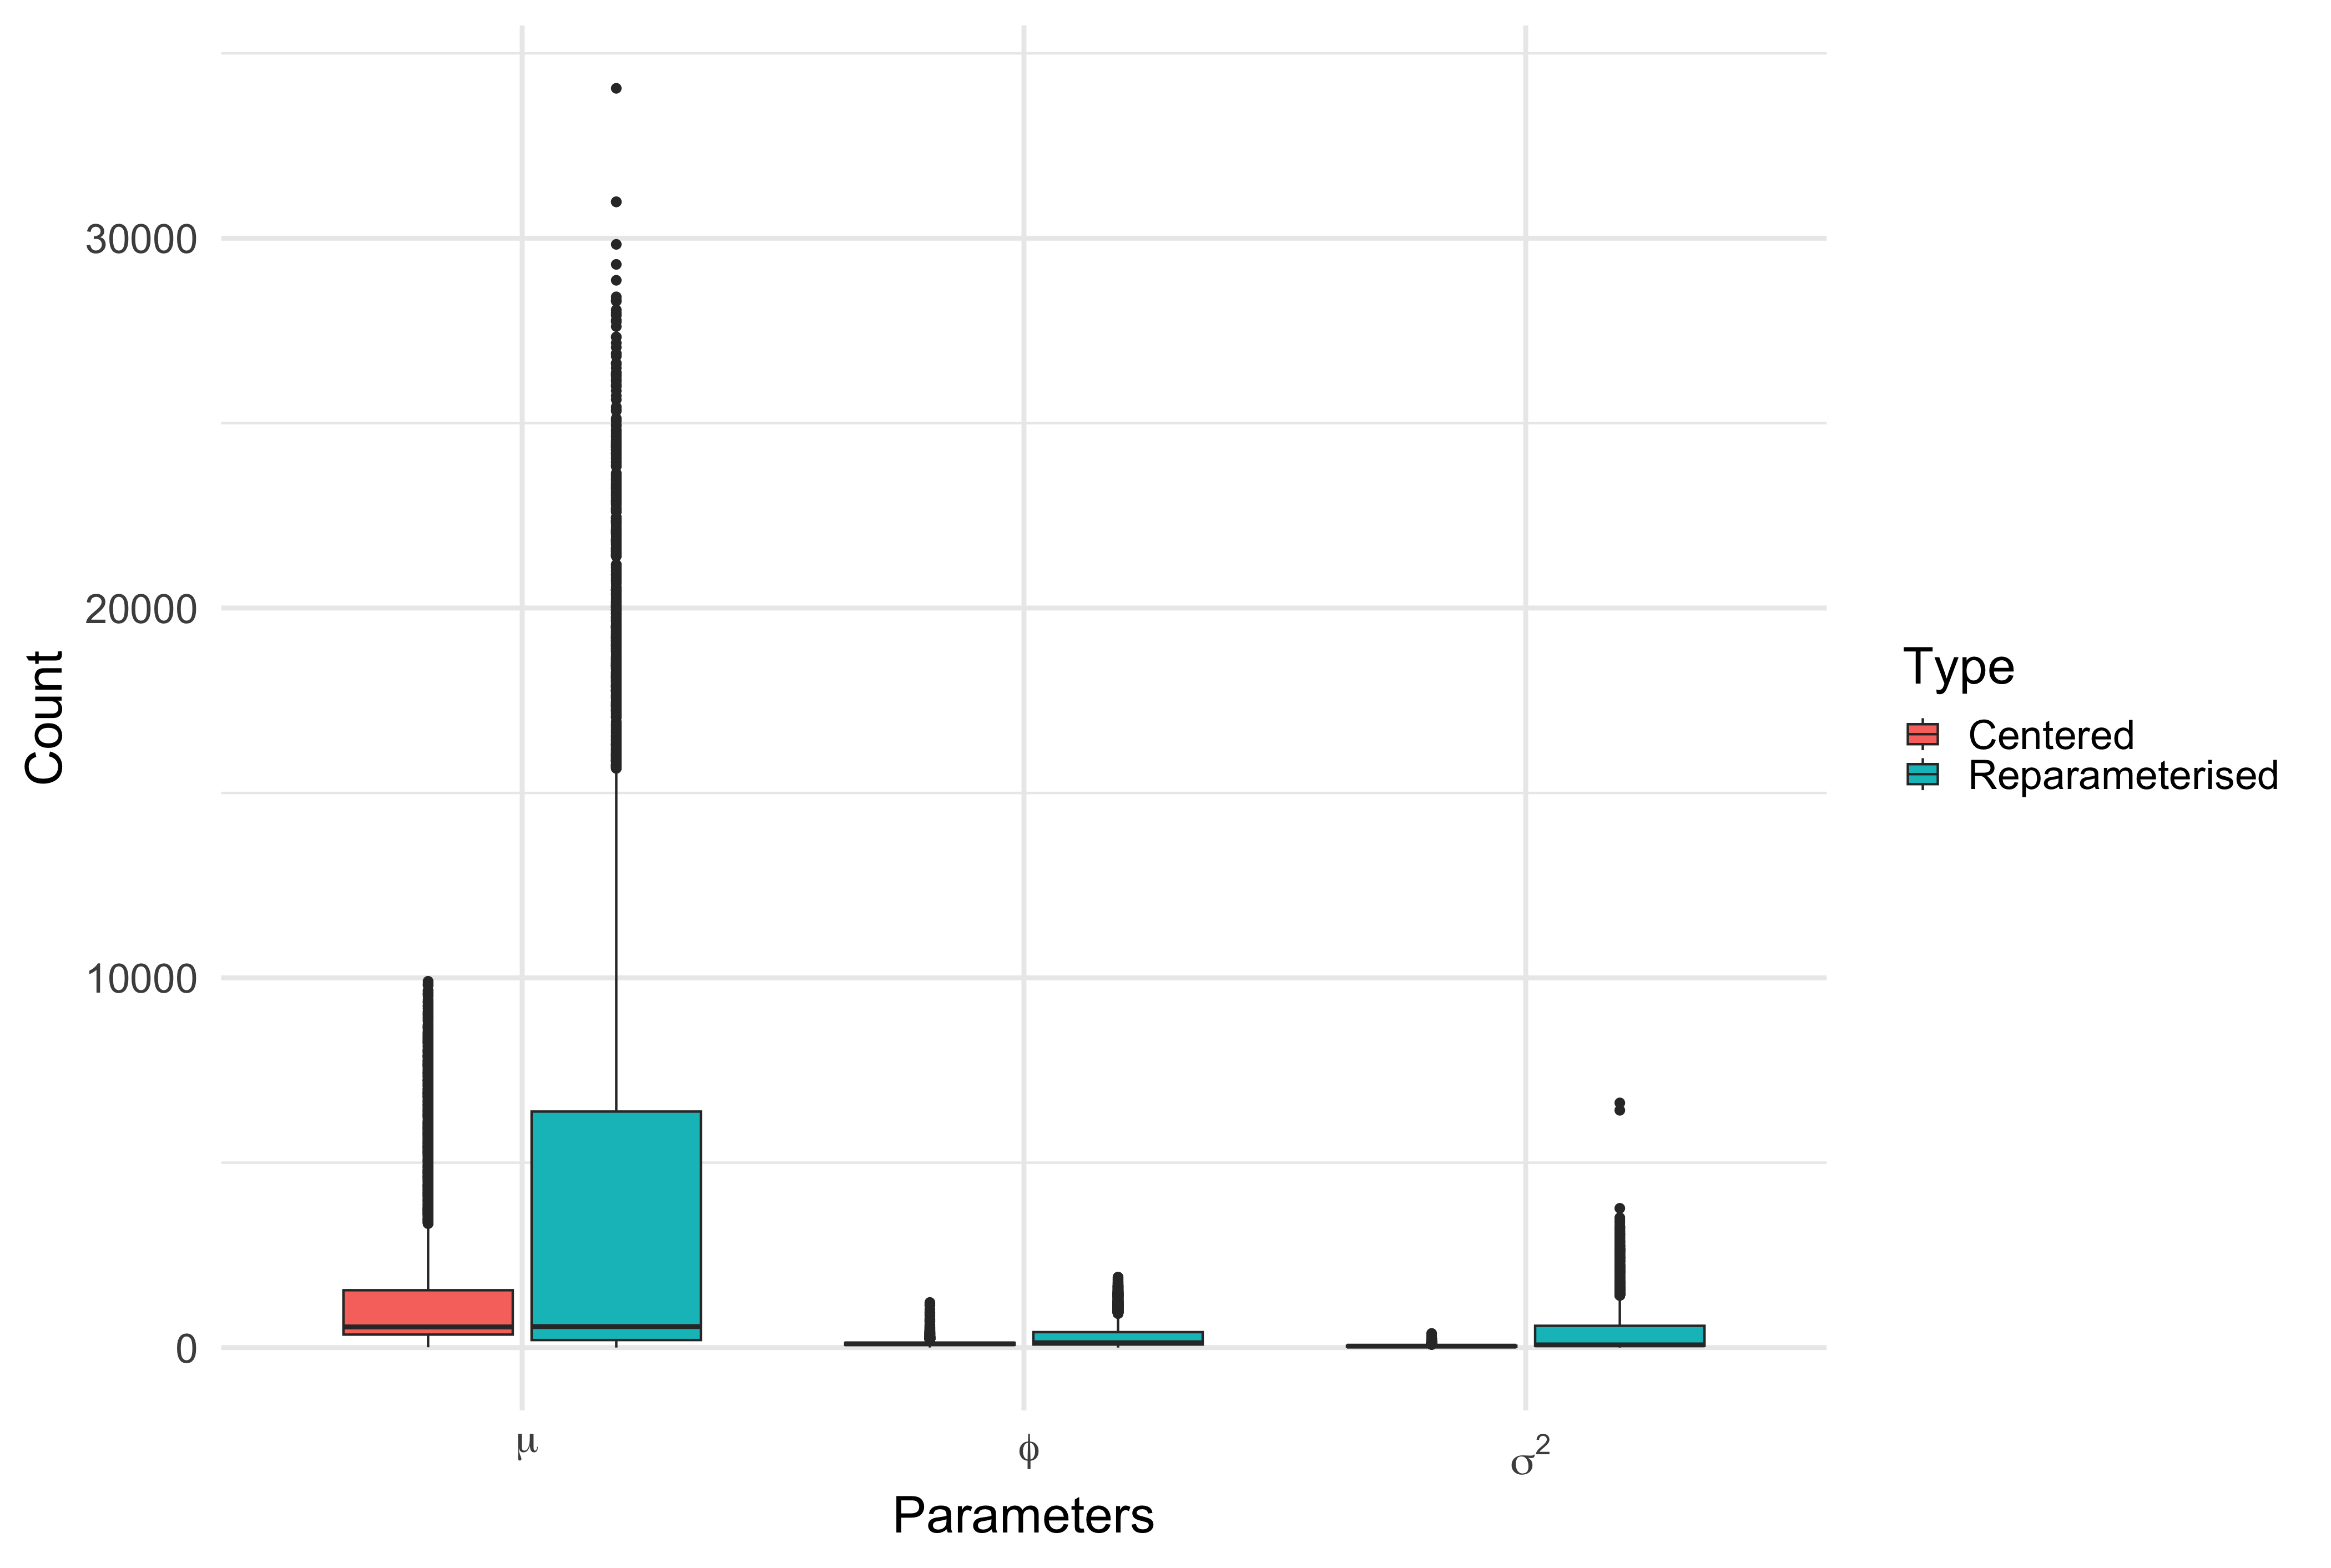
\includegraphics[scale=0.1]{results/ksc_ess.png}
        \caption{Effective sample sizes for static parameters after 5000 iterations of SBC and 1000 post burnin samples for the Gaussian Mixture model. The bespoke sampling strategy struggles to generate independent samples for all static parameters, suggesting a high degree of autocorrelation in the Markkov Chain.}
        \label{fig:kscess}
    \end{figure}

    The reparameterised model using the bespoke sampling strategy fails to generate sufficient results due to numerical errors and highly nonstationary chains. Figure X shows the traceplot from one simulation from the reparamterised model. The chain for $\phi$ is stuck to a value very close to 1 (unit root) and $\mu$ and $\sigma^2$ continuously increases in value until a numerical error is reached. Note that this occurs during the burnin phase of the markov chain. As a result, SBC is unable to be performed on this parameterisation of the model. 

    There are a variety of reasons why this may happen. Perhaps the underlying software used to perform the sampling and kalman filter is not suitable for this paramterisation, or perhaps more broadly the MCMC strategy does not perform well with this parameterisation of the model. More work is required to diagnose the cause of this problem. Other avenues to improve the sampling of this model could be to rewrite the sampler from scratch or consider a different sampling method. Note that this is only one kind of reparamterisation and further research could explore other reparamterisations, such as non centered in scale. 

    \subsection{Reweigthing rank statistics of Gaussian Mixture}
    \citet{kim1998stochastic} correct for approximation error in their method by using importance sampling weights. The reweighting procedure ensures that samples are drawn from the correct posterior density. This is applied to the calculation of the expected value of the posterior density to get a weighted mean estimate from the samples drawn from the Gaussian mixture approximation. The rank statistic can be written as a function of the expected value, so the reweighting step can be applied to the calculation of the rank statistics to see if this correction improves the calibration of the sampling approach.

    Let $v(\theta, h)$ be the log weights defined as the log difference between the posterior densities of the true model with log chi squared errors $log\: g(\theta, h | y^{\ast}_t)$ and the Gaussian mixture model $log\:  k(\theta, h_t | y^{\ast}_t)$.

    $$
    \begin{aligned}
        v(\theta, h) = log\: g(\theta, h | y^{\ast}_t) - log\:  k(\theta, h_t | y^{\ast}_t) = const + log\: g(y|h) - log\: k(y^{\ast} | h)
    \end{aligned}
    $$

    Take the exponential and normalise the weights for the $l^{th}$ posterior draw (note the constants cancel out):
    
    $$
    \begin{aligned}
    w^l = \frac{exp(v(\theta, h)_l)}{\sum_i exp(v(\theta, h)_i)}
    \end{aligned}
    $$

    This gives the importance sampling weight. The expectation for any function of the posterior samples can be written as a function of the weights.

    $$
    \begin{aligned}
    S(\theta) &= 1[\theta_l < \theta^{sim}] \\
    E[S(\theta) | y] &= \int s(\theta) g(\theta | y) d\theta\\ 
    &= \frac{\int s(\theta)\times exp(v(\theta, h)) * k(\theta, h_t | y^{\ast}_t)d\theta d h}{\int exp(v(\theta, h)) * k(\theta, h_t | y^{\ast}_t)d\theta d h} 
    \end{aligned}
    $$

    Therefore, the expectation of the reweighted posterior samples is given by:

    $$
    \begin{aligned}
    E[S(\hat{\theta}) | y^{\ast}] = \sum_l^L S(\hat{\theta}_l)w_l
    \end{aligned}
    $$

    The rank statistic can be rewritten as a function of the expectation and weights. This gives us the reweighted rank statistics.

    $$
    \begin{aligned}
    r = \sum_{l=1}^{L}1[\theta_{l} < \theta^{sim}] \approx  L\times E[S(\hat{\theta})] = L\times \sum_l^L S(\theta_l)w_l
    \end{aligned}
    $$

    The results from applying this reweighting step to the rank statistics are given on Figure \ref{fig:reweight1k}. There are no major improvements to the uniformity of rank statistics. Increasing the SBC iterations to 5000 as seen in Figure \ref{fig:reweight5k} also results in no major improvements. The shape of both sets of histograms is consistent with the shape of the unweighted rank statistics. 

    \begin{figure}[H]
        \centering
        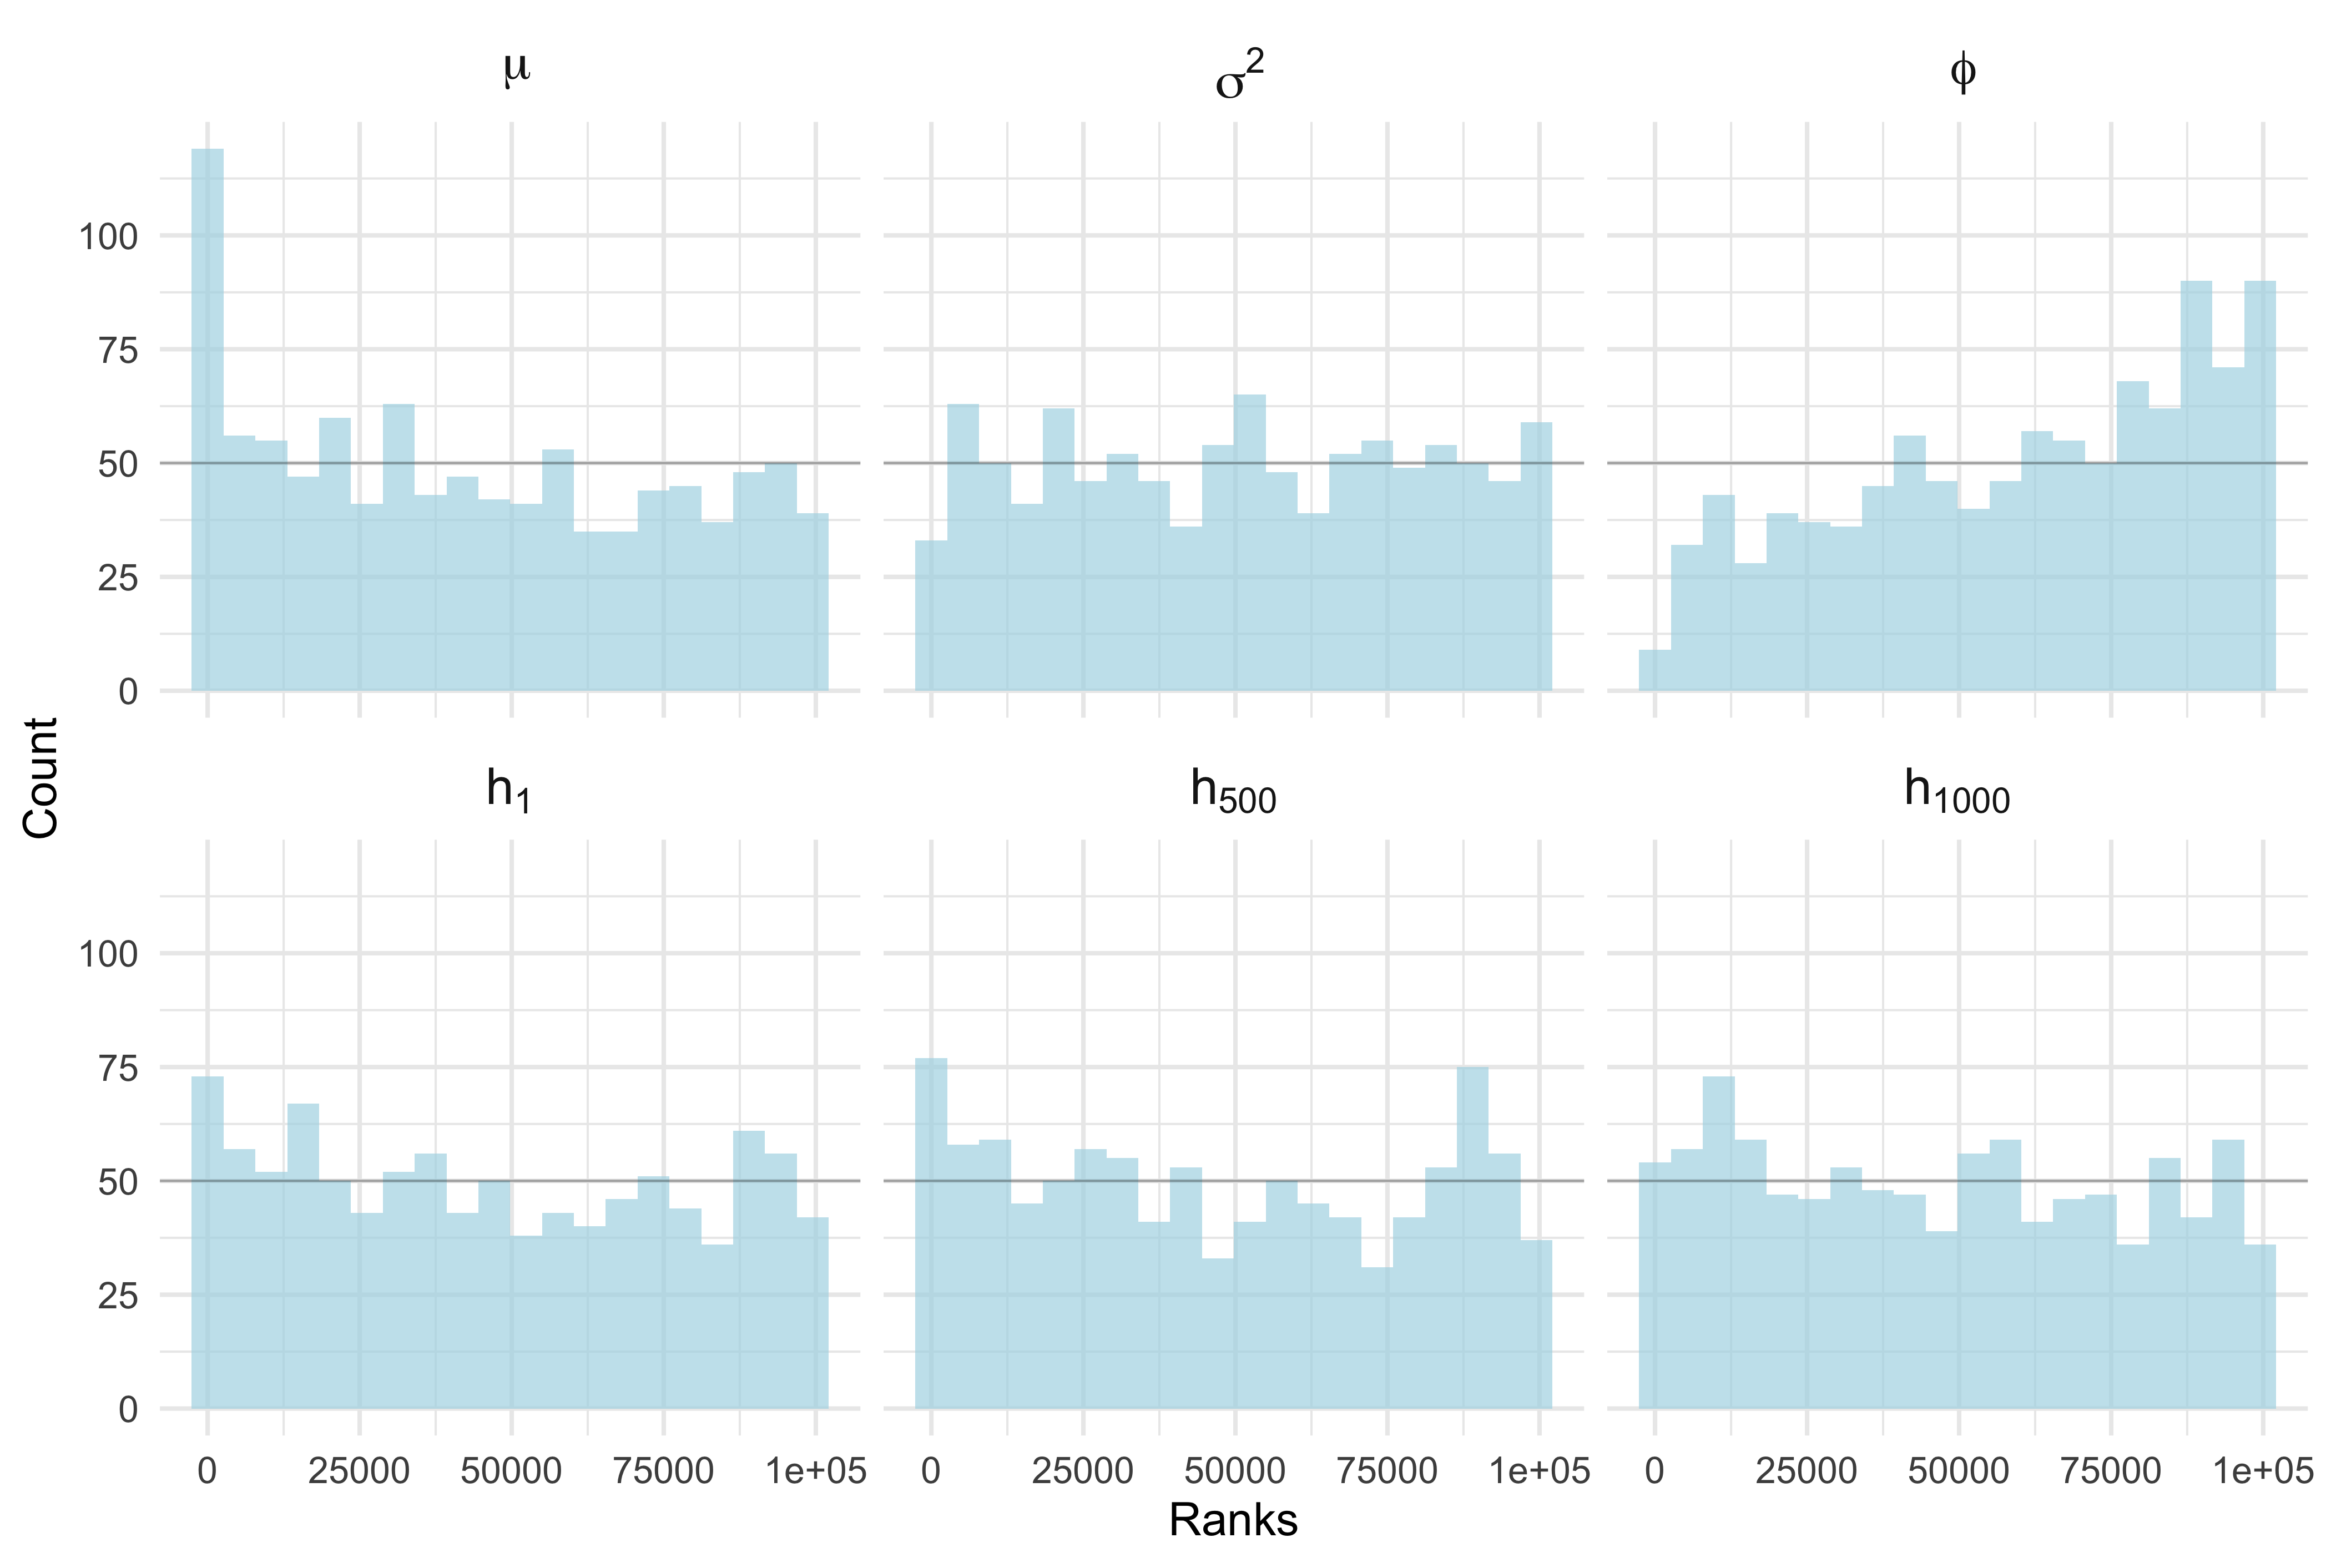
\includegraphics[scale=0.1]{results/sir_cp_1k.png}
        \caption{1000 SBC iterations for reweighted rank statistics from the Gaussian mixture approximation model. The shape of the histogram is consistent with the unweighted rank statistics.}
        \label{fig:reweight1k}
    \end{figure}

    \begin{figure}[H]
        \centering
        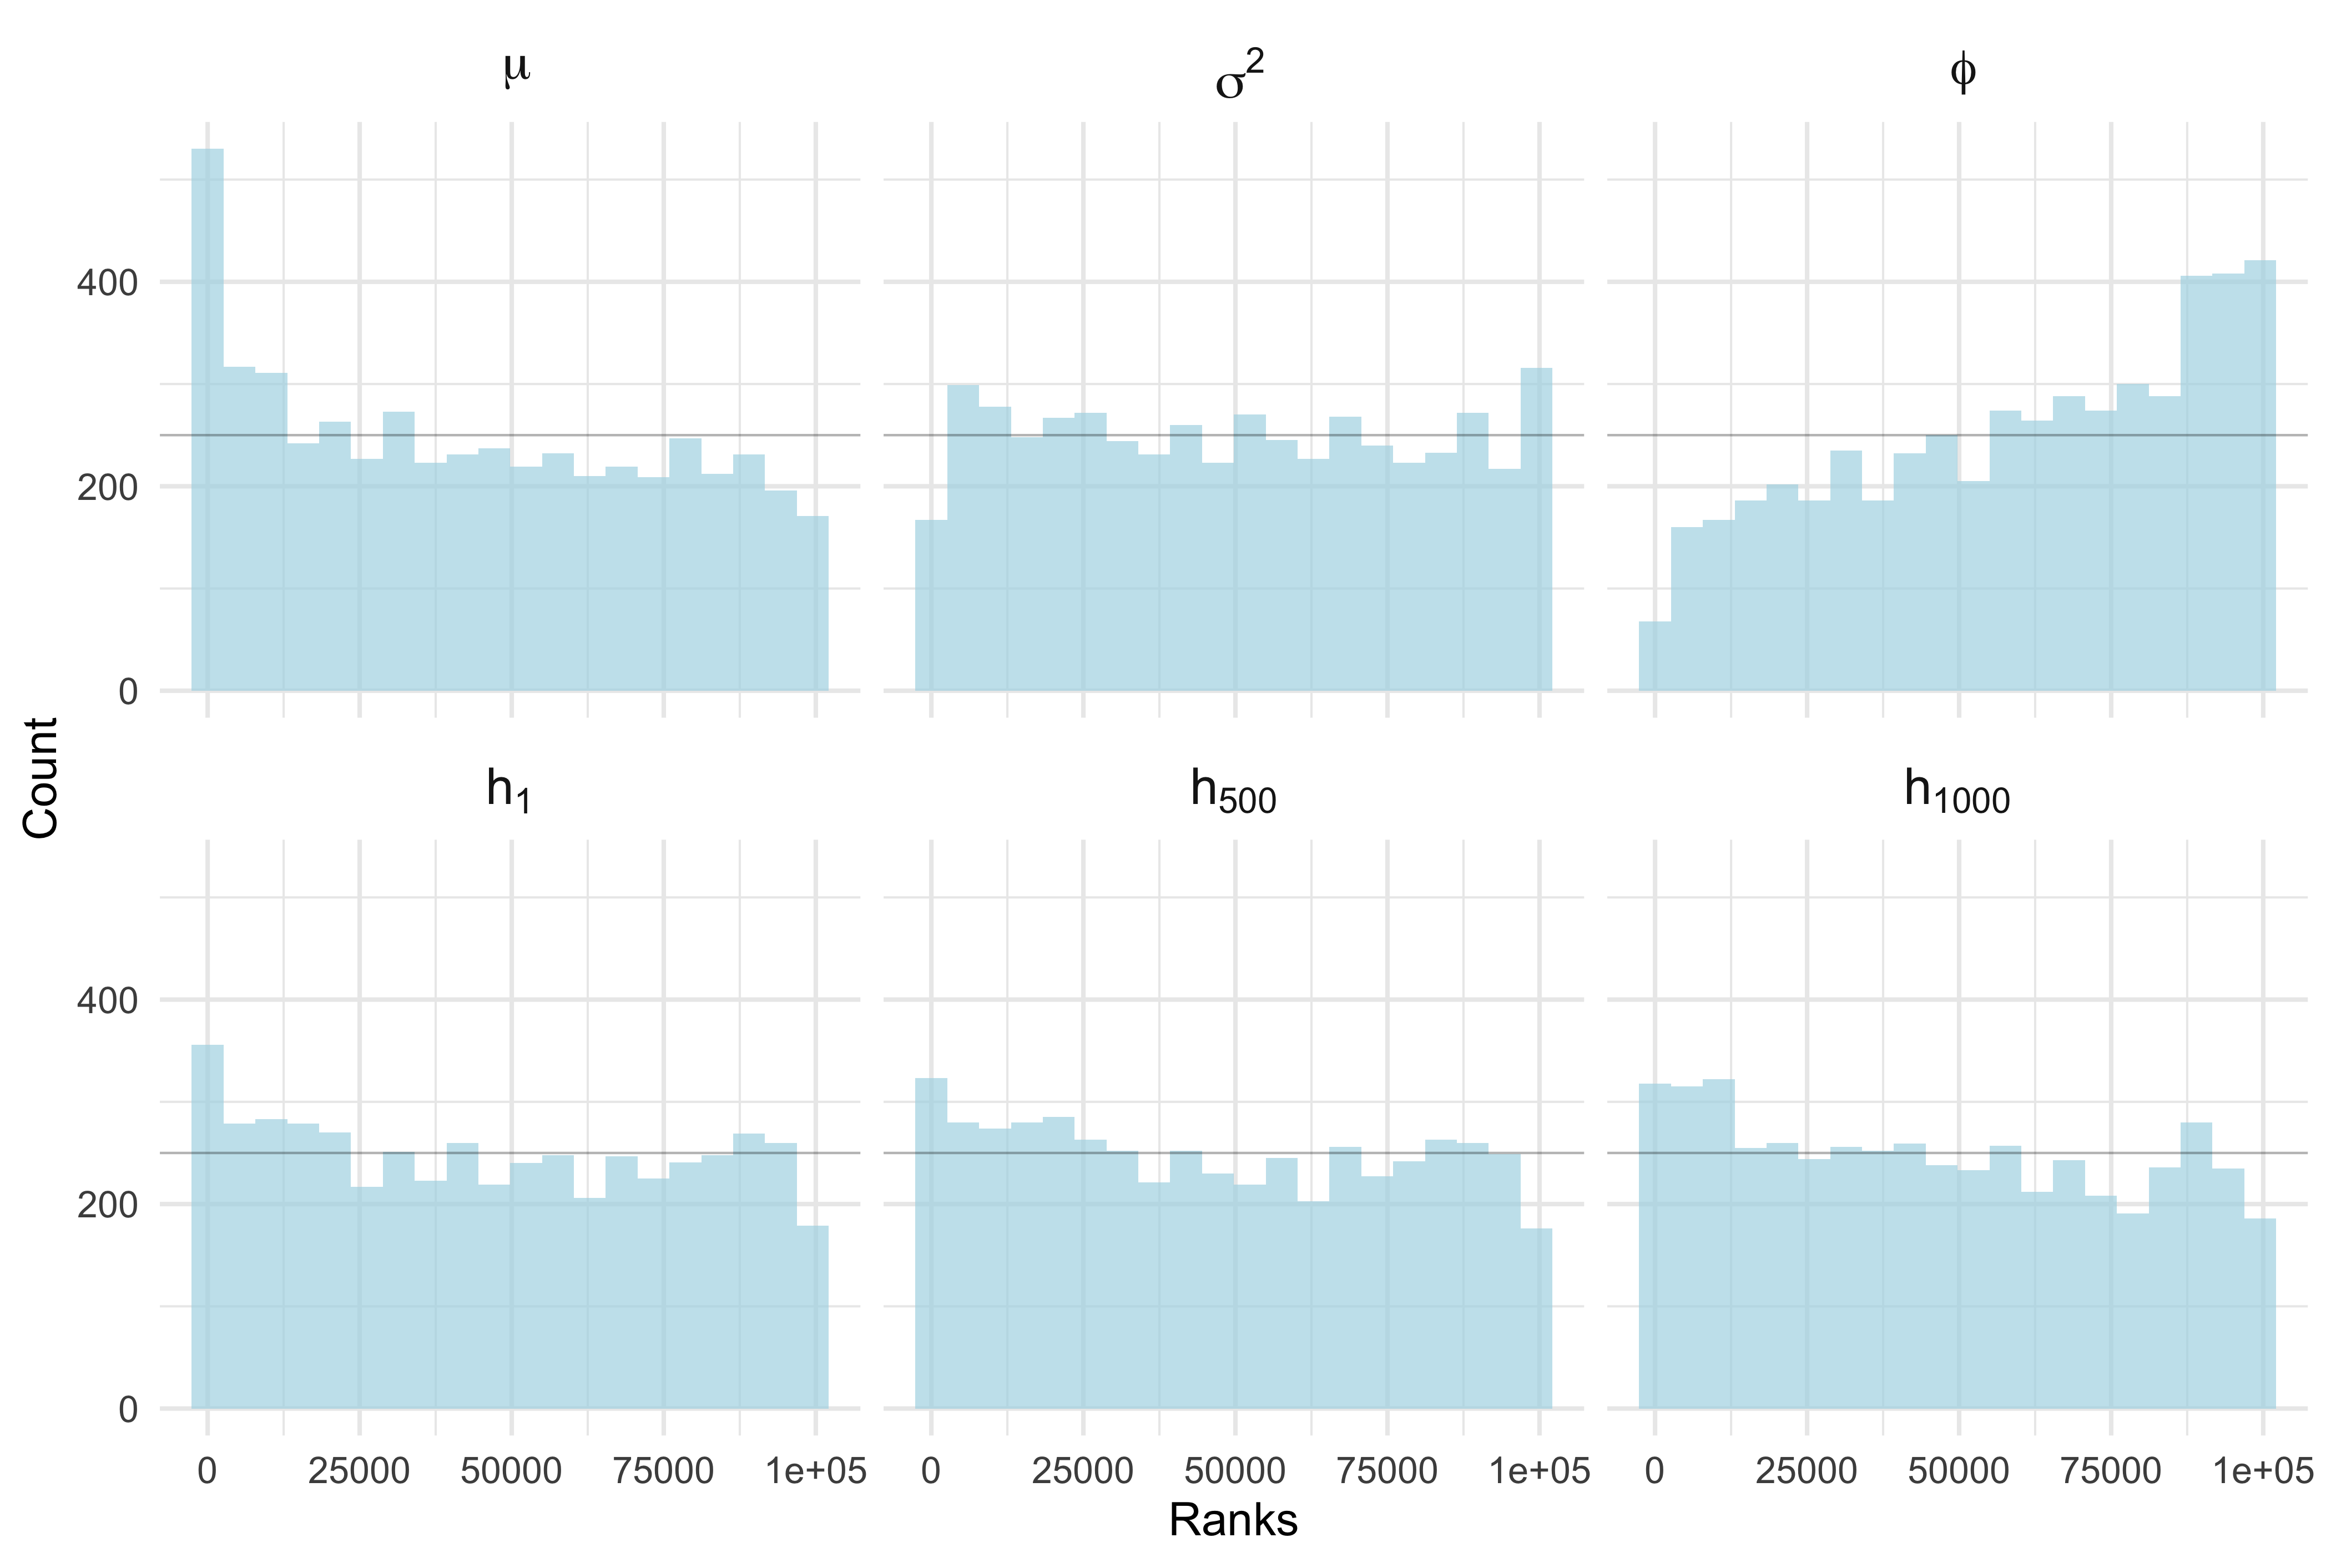
\includegraphics[scale=0.1]{results/sir_cp_5k.png}
        \caption{5000 SBC iterations for reweighted rank statistics from the Gaussian mixture approximation model. No major improvements are observed to the uniformity of rank statistics.}
        \label{fig:reweight5k}
    \end{figure}

    \subsection{Evaluating all models and parameters}
    As discussed, it is not practical to visually inspect the histograms of all parameters in the stochastic volatility model. Instead, the Chi squared statistic can be used to summarise the shape of the distribution and if desired, be used for hypothesis testing. However, instead of performing hypothesis tests, another visual approach is taken to compare the calibration of the algorithms and parameters. 
    % However, performing all these tests suffers from the same overcommunication as presenting all the histograms at once.

    The distribution of chi squared statistics across all simulations and all parameters are plotted as histograms on Figure \ref{fig:allchisq}. A chi squared statistic of 0 implies the sample is exactly uniformly distributed. Any value away from 0 captures any variation or deviation away from uniformity. This provides a high level view of all parammeters - how close they are to uniformity and how close or far away they are relative to the other SBC results for other algorithms and parameterisations. 

    \begin{figure}[H]
        \centering
        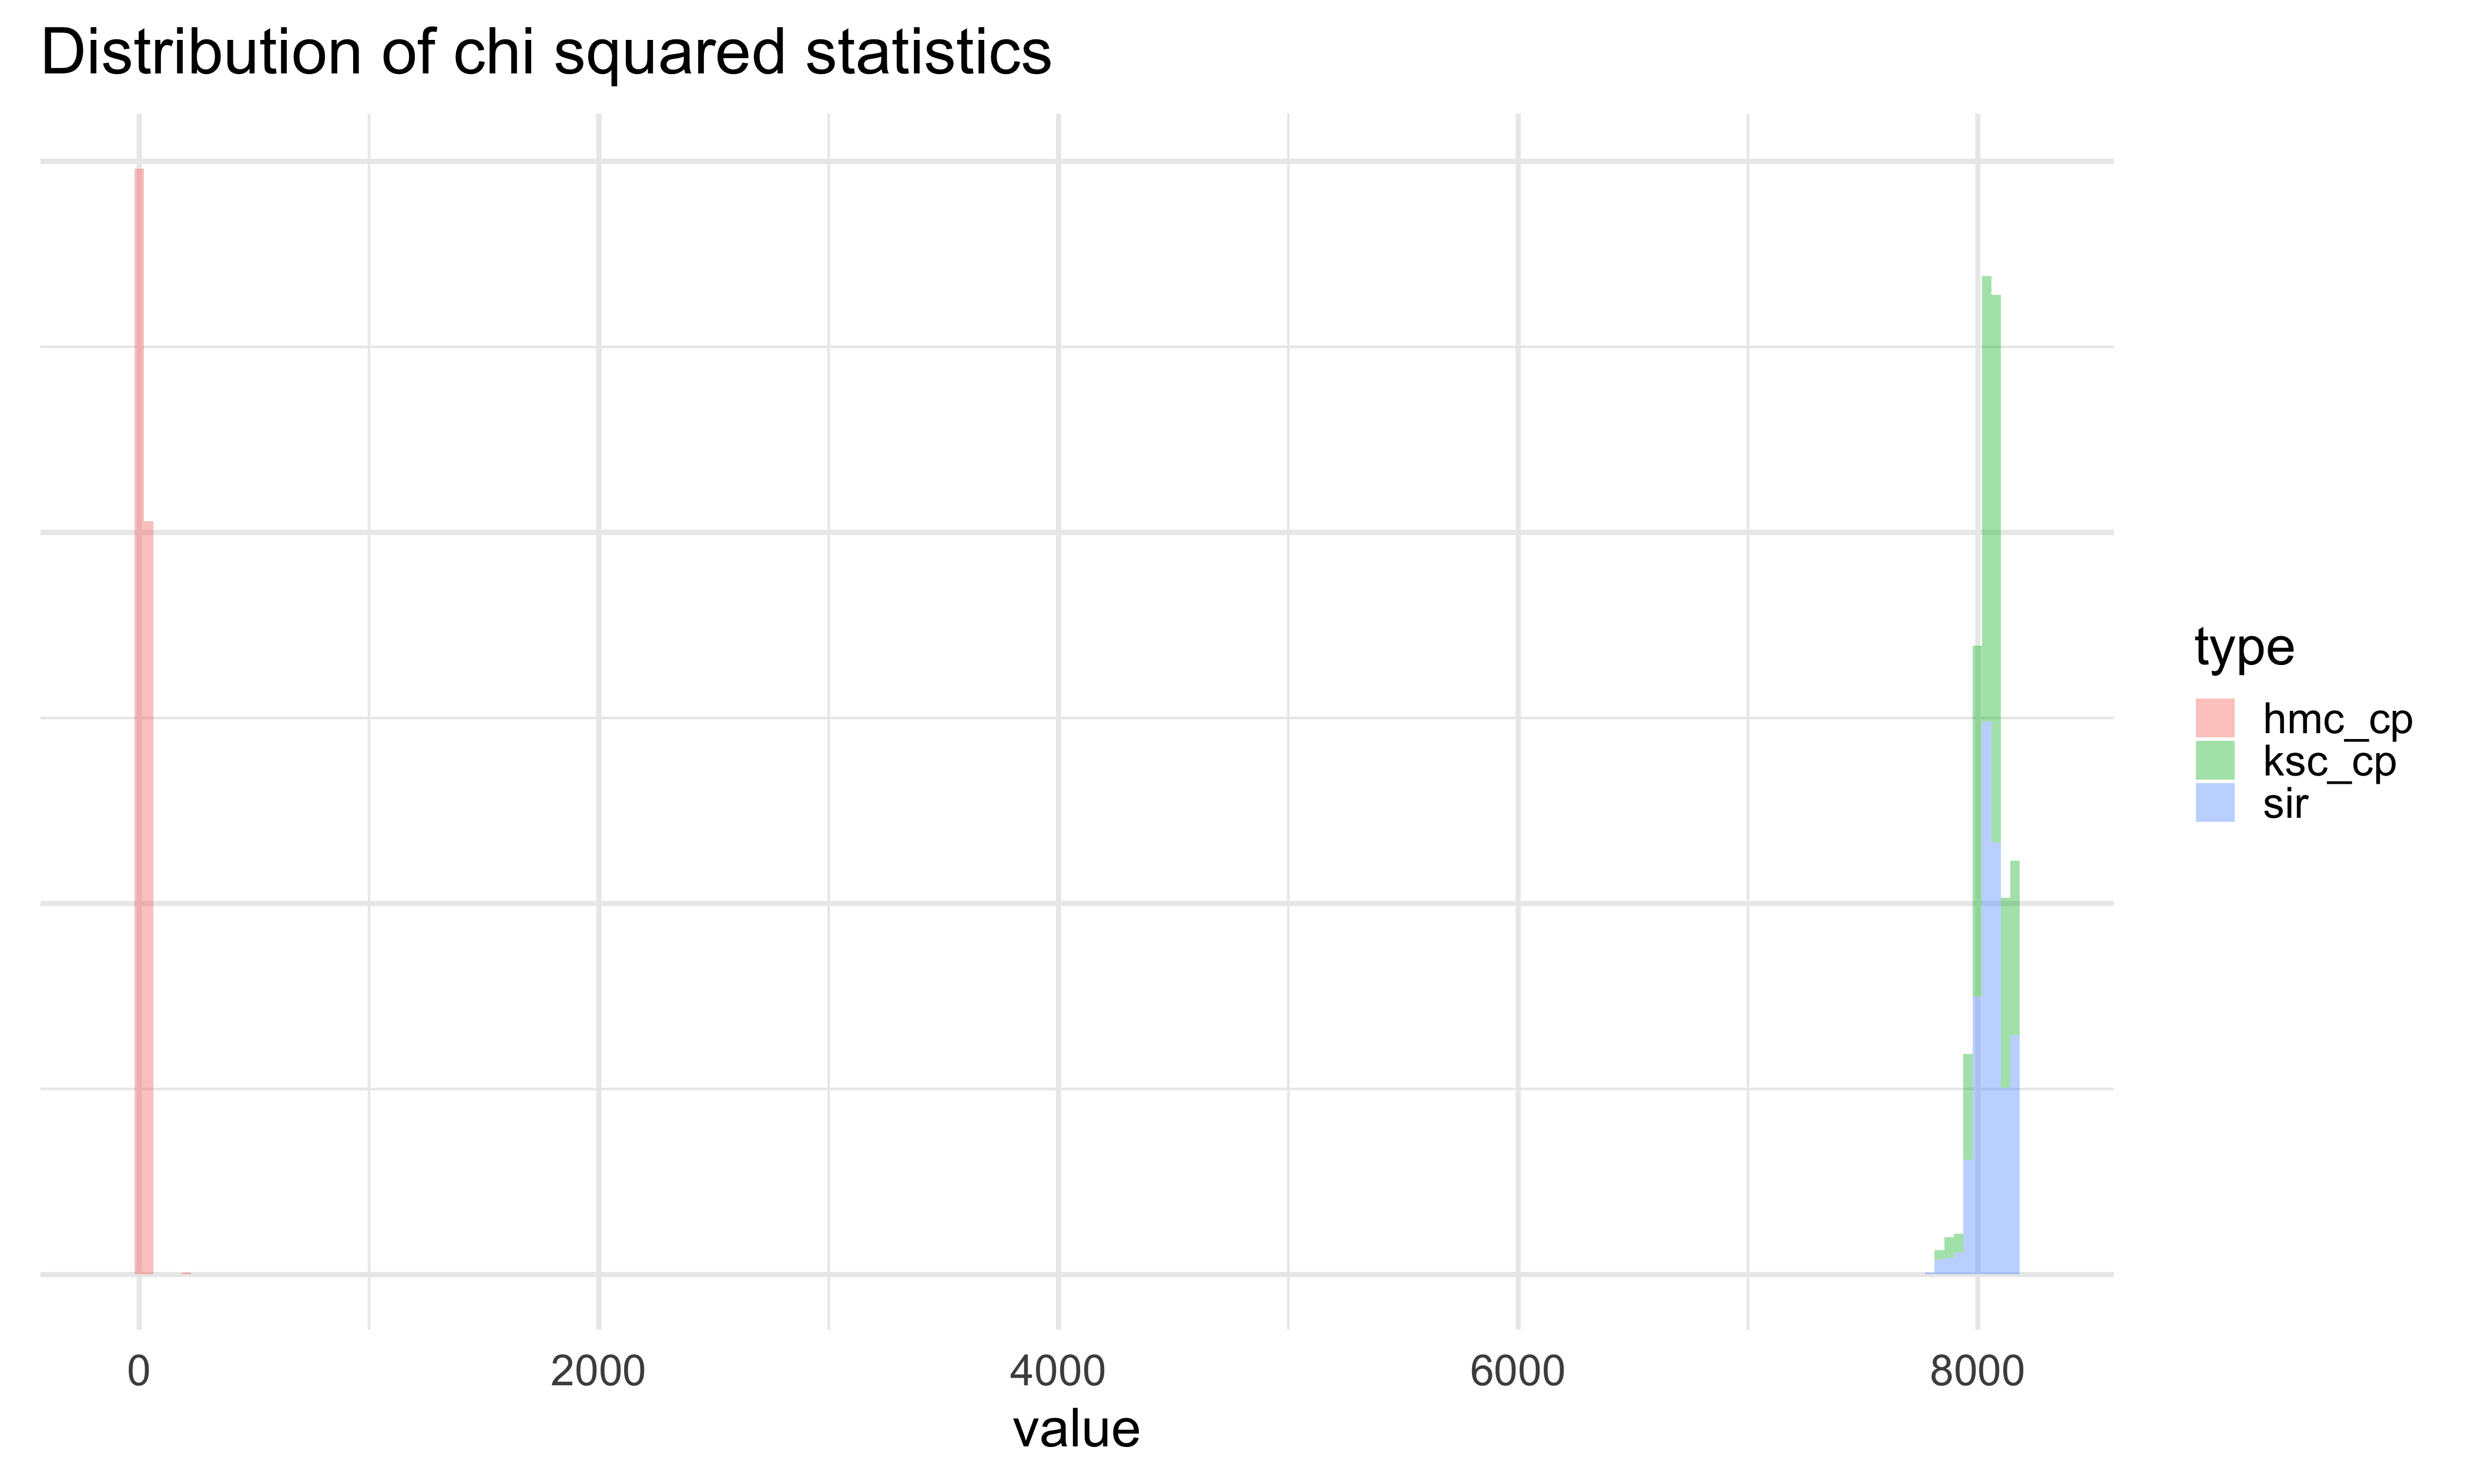
\includegraphics[scale=0.1]{results/dist_chisq.png}
        \caption{Distribution of chi squared statistics for all models (5000 SBC iterations).}
        \label{fig:allchisq}
    \end{figure}

    The distribution for HMC are clustered very closely to zero. Both results for the bespoke sampling method are distributed far from zero which suggests strong evidence of a lack of uniformity across all parameters. This is consistent with the distribution of rank statistics in the previous sections. 

\section{Discussion}
Overall, Hamiltonian Monte Carlo applied on the reparameterised model performed best based on the calibration and efficiency evaluation criteria. Centered parameterisation using HMC performed moderately well but struggled to produce calibrated posterior estimates for $\sigma^2$ and $\phi$ as well as generate independent samples for these parameters. Gaussian mixture approximation struggled to return calibrated posterior estimates and efficient samples for both parameteristions. However, the centered parameteristion results for the Gaussian mixture model may improve if we increased the length of the Markov chain. This is discussed later in the limitations section. 

These results demonstrate that the performance of a MCMC algorithm is sensitive to the paramterisation of the model in the context of calibration and efficiency. Furthermore, the paramterisation of a model is conditional on the choice of MCMC algorithm. Evaluating the effectiveness of a modelling strategy (i.e choice of model, paramterisation and sampler) on simulated data gives a lot of a priori information about how the model will perform before it is fit on real data. Performing SBC may help isolate confounding factors if any problems occur. 

The priors chosen for this study came directly from \citet{kim1998stochastic}. The SBC results for the Gaussian mixture may improve if the priors were more informative - although this is only conjecture. Whether or not to use tighter priors depends on the modelling context and the problem at hand. If the model is expected to handle datasets generated by a set of priors, then uncalibrated results from SBC raises questions about the suitability about the model choice, MCMC or parameterisation. 

Other parameterisaions of the stochastic volatility model are available as outlined in \citet{strickland2008parameterisation}, namely non centered in scale or both non centered in scale and location. The failure of non centered parameterisaion in location for the Gaussian mixture model could be due to a variety of reasons. This may be due to a particular software implementation when it comes to the Kalman Filter and Simulation Smoother (in which a specific software package was applied) that was not designed to handle the non centered parameterisations. Or perhaps this particular parameterisation doesn't suit the sampling strategy applied by KSC and another approach (e.g. HMC) might be more successful. Lots of different design and implementation details could be explored further. Pinpointing the reason why this model parameterisation failed as well as exploring other configurations and MCMC algorithms in this context is left to future research.

It is worth noting that there are many ways of "comparing" MCMC approaches. Other features that may be of interest is the speed in which a MCMC can converge onto the target distribution and generate samples for inference. However, "speed" is diffiuclt to define and is subject to a variety of different factors such as hardware, operating system, etc. The purpose of this research is to compare algorithms based on calibration and efficiency. Additionally, this simulation study does not provide any advice on the appropriateness of the stochastic volatility model on real data. Whether the stochastic volatility model is appropriate for modelling a particular financial time series requires further study into the data generating process, domain expertise and a suite of other diagnostic checks. Examples of this are posterior predictive checking and out of sample predictive performance. Rather, ths SBC approach gives insight into how well calibrated a sampling strategy is conditional on a known data generating process which is important in all applied contexts.  

% (other implementations exist as well but left for future research. lots of different design and implementation details could be explored. Let alone choice of algos.)

\section{Limitations}
A limitation to applying SBC in all modelling contexts is that it is computationally intensive. SBC requires fitting multiple models to get reliable estimates. In some cases, fitting just one model can take a long time, let alone multiple. Producing results for this research within a reasonable timeframe required use of a computer cluster. Computing infrastructure may limit the opportunity for SBC to be performed,although it is probably not necessary to do 5000 SBC iterations in other research contexts. The choice of SBC iterations for this research was arbitrary and was used to demonstrate that noisy estimates could be reduced by increasing the number of iterations for calibrated models. A more principlied approach to picking the number of SBC iterations could be explored in other research.

Developing diagnostic tools for evaluating SBC results and models with many parameters is an area for improvement. As discussed, inspecting many histograms for highly parameterised models is unrealistic. Other summary statistics and visualisations can be applied for a high level comparison, such as the chi squared statistics applied in this research. Furthermore, it is not always straightforward to understand why any any one parameter may produce poor calibration results, for example, an arbitrary state parameter. SBC may tell us some information about the miscalibration based on the histogram shape (e.g. under or over dispersed relative to the prior distribution), but understanding why this occurs may not be straight forward. Although, diagnosing sampling problems with complicated posterior geometries speaks more generally to the difficulty of understanding complex models in the first place as opposed to a limitation of SBC.

Lastly, it is unclear what constitutes a "fair comparison" between algorithms when comparing SBC results. In particular, the number of post burnin or warmup samples differed between algorithms (999 post burn-in for HMC, 9999 for the bespoke algorithm). An argument could be made that the poor results for the bespoke algorithm may be due to the chain not converging onto the target distribution. Indeed, the authors of this approach extended their Markov chain to 750,000 posterior draws. A farier comparison may be to have roughly similar number of ESS for most of the estimated parameters, although this is difficult to get right with multiple parameters. However, given how well Hamiltoninan Monte Carlo performed with the reparamterised model, any improvement to the Gaussian mixture model by increasing the length of the Markov chain would make calibration just as good, but not better due to the inefficiency of the sampler. 

\section{Conclusion}
This research evaluated and compared different MCMC algorithms for fitting stochastic volatility models. As our models and algorithms for estimating these models become more complicated, so does the need for principled ways of checking that they are returning correct posterior estimates. SBC provides a general simulation design for generative models to check whether a modelling strategy is producing the correct posterior estimates. 

In the context of stochastic volatility, applying Hamiltonian Monte Carlo on a reparameterised stochastic volatility model provided the most calibrated and efficient estimates when compared to the bespoke sampling method using a Gaussian mixture model. This also outperformed SBC and ESS results when using importance sampling weights to correct for approximation error. Other parameterisations of the stochastic volatility model can be considered to see if it improves sampling performance based on these metrics. 

This study only considered a handful of potential algorithms, sampling strategies and parameterisations for stochastic volatility. Future research could use the same SBC design to compare and evaluate more complicated volatility models (or any model outside this domain) and MCMC approaches. Overall, SBC can be applied as part of the development of various probabilistic and Bayesian models and is a useful tool as part of a statistical workflow.
 
\newpage

\bibliography{references}

\end{document}
